\pdfobjcompresslevel 0
\documentclass[10pt, a4paper, parskip=full, twoside, twocolumn]{report}

% --- PREAMBULE ---
\usepackage[utf8]{inputenc}
\usepackage[T1]{fontenc}
\usepackage[french]{babel}
\usepackage{amsmath, amssymb, amsthm, amsfonts}
\usepackage[top=1cm,bottom=2cm,left=1cm,right=1cm]{geometry}
\usepackage{graphicx}
\usepackage{stmaryrd}
\usepackage{xcolor}
\usepackage{framed}
\usepackage{enumitem}
\usepackage{titlesec}
\usepackage{aliascnt}
\usepackage{quiver}
\usepackage{algpseudocode}
\usepackage{tcolorbox} % The main package for creating the colored box
\tcbuselibrary{breakable}

% Define a custom color (optional, but good practice)
\definecolor{mygreen}{rgb}{0.2, 0.7, 0.2}
\definecolor{myblue}{rgb}{0.0, 0.2, 0.7}
\definecolor{myred}{rgb}{0.7, 0.2, 0.2}
\definecolor{paragraphtext}{rgb}{0.4, 0.3, 0.9}
\definecolor{developpement}{RGB}{255, 255, 224}

% Apply the color to the subsection title
\titleformat{\section}
  {\normalfont\large\bfseries\color{myred}} % The format for the whole line
  {\thesection}                           % The subsection number
  {1em}                                      % Separation between number and title
  {}                                         % Code before the title text (empty for now)

% Apply the color to the subsection title
\titleformat{\subsection}
  {\normalfont\large\bfseries\color{mygreen}} % The format for the whole line
  {\thesubsection}                           % The subsection number
  {1em}                                      % Separation between number and title
  {}                                         % Code before the title text (empty for now)
  
\newtheorem{definition}{Définition}
\newtheorem{theorem}[definition]{Théorème}
\newtheorem{theorem_def}[definition]{Théorème/Définition}
\newtheorem{proposition}[definition]{Proposition}
\newtheorem{proposition_def}[definition]{Proposition/Définition}
\newtheorem{properties}[definition]{Propriétés}
\newtheorem{property}[definition]{Propriété}
\newtheorem{lemma}[definition]{Lemme}
\newtheorem{lemma_def}[definition]{Lemme/Définition}
\newtheorem{corollary}[definition]{Corollaire}
\newtheorem{corollary_def}[definition]{Corollaire/Définition}
\newtheorem{example}[definition]{Exemple}
\newtheorem{cexample}[definition]{Contre-exemple}
\newtheorem{remark}[definition]{Remarque}
\newtheorem{application}[definition]{Application}
\newtheorem{reference}[definition]{Référence}
\newtheorem{algorithm}[definition]{Algorithme}
\newtheorem{conjecture}[definition]{Conjecture}
\newtheorem{notation}[definition]{Notation}
\newtheorem*{notation*}{Notation}
\newtheorem*{example*}{Exemple}

\newcommand{\IN}{\mathbb{N}}
\newcommand{\IZ}{\mathbb{Z}}
\newcommand{\IU}{\mathbb{U}}
\newcommand{\IK}{\mathbb{K}}
\newcommand{\IP}{\mathbb{P}}
\newcommand{\IE}{\mathbb{E}}
\newcommand{\IV}{\mathbb{V}}
\newcommand{\IZnZ}{\mathbb{Z}/n\mathbb{Z}}
\newcommand{\IZpZ}{\mathbb{Z}/p\mathbb{Z}}
\newcommand{\IQ}{\mathbb{Q}}
\newcommand{\IC}{\mathbb{C}}
\newcommand{\IF}{\mathbb{F}}
\newcommand{\IR}{\mathbb{R}}
\newcommand{\IRn}{\mathbb{R}^n}
\newcommand{\IRd}{\mathbb{R}^d}
\newcommand{\IRm}{\mathbb{R}^m}
\newcommand{\IRp}{\mathbb{R}^p}
\newcommand{\IRnm}{\mathbb{R}^{n\times m}}
\newcommand{\IRmn}{\mathbb{R}^{m\times n}}
\newcommand{\IRpn}{\mathbb{R}^{p\times n}}
\newcommand{\IRnp}{\mathbb{R}^{n\times p}}
\newcommand{\IRpm}{\mathbb{R}^{p\times m}}
\newcommand{\IRmp}{\mathbb{R}^{m\times p}}
\newcommand{\M}{\mathcal{M}}
\newcommand{\B}{\mathcal{B}}
\newcommand{\A}{\mathcal{A}}
\newcommand{\actson}{\circlearrowleft}

\DeclareMathOperator{\im}{Im}
% \DeclareMathOperator{\Im}{Im}
\DeclareMathOperator{\pgcd}{pgcd}
\DeclareMathOperator{\ppcm}{ppcm}
\DeclareMathOperator{\rg}{rg}
\DeclareMathOperator{\rang}{rang}
\DeclareMathOperator{\card}{Card}
\DeclareMathOperator{\Is}{Is}
\DeclareMathOperator{\Orb}{Orb}
\DeclareMathOperator{\Stab}{Stab}
\DeclareMathOperator{\Fix}{Fix}
\DeclareMathOperator{\Supp}{Supp}
\DeclareMathOperator{\ord}{ord}
\DeclareMathOperator{\Ker}{Ker}
\DeclareMathOperator{\Syl}{Syl}
\DeclareMathOperator{\Mat}{Mat}
\DeclareMathOperator{\id}{id}
\DeclareMathOperator{\diag}{diag}
\DeclareMathOperator{\car}{car}
\DeclareMathOperator{\Hom}{Hom}
\DeclareMathOperator{\Aut}{Aut}
\DeclareMathOperator{\End}{End}
\DeclareMathOperator{\Div}{Div}
\DeclareMathOperator{\Frac}{Frac}
\DeclareMathOperator{\Vect}{Vect}
\DeclareMathOperator{\tr}{tr}
\DeclareMathOperator{\Com}{Com}
\DeclareMathOperator{\Sp}{Sp}
\DeclareMathOperator{\Cov}{Cov}
\DeclareMathOperator{\Hess}{Hess}

\titleformat{\chapter}[display]
  {\normalfont\bfseries}{}{0pt}{\LARGE}
\titlespacing*{\chapter}{0pt}{0pt}{\baselineskip}

\newcommand{\vertiii}[1]{{\left\vert\kern-0.25ex\left\vert\kern-0.25ex\left\vert #1 
    \right\vert\kern-0.25ex\right\vert\kern-0.25ex\right\vert}}

\title{Leçons d'oral de l'Agrégation}
\author{Gautier Laisné}
\date{}


\begin{document}
% \maketitle
% \tableofcontents

\chapter{101 : Groupe opérant sur un ensemble. Exemples d'applications.}
Dans cette leçon, $G$ désigne un groupe de neutre $1$, et $X$ désigne un ensemble.
\section*{I. Action d'un groupe sur un ensemble}
\subsection*{A. Définitions et premiers exemples}
\begin{definition}[\textnormal{[R] 19, [U] 27}]
	Une \emph{action} de $G$ sur $X$ est une application $G\times X\to X$ définie par 
	$(g,x)\mapsto g\cdot x$ vérifiant
	\begin{enumerate}
		\item $\forall\, (g,g')\in G^2,\, \forall\, x\in X,\, g'\cdot (g\cdot x) = (g'g)\cdot x$
		\item $\forall\, x\in X,\, 1\cdot x = x$
	\end{enumerate}
	Pour signigier que $G$ agit sur $X$, on note $G\actson X$.
\end{definition}

\begin{example}[\textnormal{[R] 19, [U] 28}]
	\begin{itemize}
		\item $\mathfrak{S}(X) \actson X$ par $\sigma\cdot x = \sigma(x)$
		\item Si $E$ est un espace vectoriel, alors $GL(E)\actson E$ par $\varphi\cdot x = \varphi(x)$
		\item $(g,x)\mapsto x$ est une action de $G$ sur $X$, appelée \emph{action triviale}.
	\end{itemize}
\end{example}

\begin{proposition}[\textnormal{[R] 19, [U] 28}]
	La donnée d'une action $(g,x)\mapsto g\cdot x$ de $G$ sur $X$ équivaut à la donnée d'un morphisme $\varphi\,\colon G\to \mathfrak{S}(X)$, $g\mapsto \left[x\mapsto g\cdot x\right]$, appelé \emph{morphisme associé à l'action de $G$ sur $X$}.
\end{proposition}

\begin{definition}[\textnormal{[R] 19/21, [U] 29}]
	Soit $x\in X$. Alors :
	\begin{itemize}
		\item L'\emph{orbite} de $x$ est l'ensemble $\Orb(x) = \left\{g\cdot x \mid g\in G\right\}$ (aussi noté $G\cdot x$) ;
		\item Le \emph{stabilisateur} de $x$ est l'ensemble $\Stab(x) = \left\{g\in G \mid g\cdot x = x\right\}$.
	\end{itemize}
\end{definition}

\begin{proposition}[\textnormal{[U] 34/37}]
	\begin{enumerate}
		\item $G\actson G$ par $g\cdot h=ghg^{-1}$ (on l'appelle \emph{action par conjugaison}). Le stabilisateur de $h\in G$ est appelé \emph{centralisateur} de $h$, et est noté $C(h)$.
		\item $G$ agit sur l'ensemble de ses sous-groupes par $g\cdot H = gHg^{-1}$ (action par conjugaison). Le stabilisateur de $H\leq G$ est appelé \emph{normalisateur} de $H$, et est noté $N(H)$.
	\end{enumerate}
\end{proposition}

\begin{definition}[\textnormal{[R] 20, [U] 29/31}]
	On dit que l'action de $G$ sur $X$ est \emph{transitive} si elle n'a qu'une seule orbite, \emph{i.e.} si $\forall\,(x,y)\in X^2,\, \exists\, g\in G\,\colon g=g\cdot x$.

	On dit que l'action de $G$ sur $X$ est \emph{fidèle} si $\varphi$ est injective.
\end{definition}

\begin{example}[\textnormal{[U] 31}]
	\begin{itemize}
		\item $\mathfrak{S}_n\actson \llbracket 1,n\rrbracket$ transitivement par $\sigma\cdot i=\sigma(i)$
		\item $G\actson G$ fidèlement par $g\cdot h = gh$ (on l'appelle \emph{action par translation à gauche})
		\item Soit $H$ un sous-groupe de $G$. L"'action de $G$ sur $G/H$ définie par $g\cdot xH = gxH$, appelée \emph{action par translation à gauche}, est transitive.
	\end{itemize}
\end{example}

\begin{proposition}[\textnormal{[R] 21}]
	Pour tout $x\in X$, $\Stab(x)$ est un sous-groupe de $G$.
\end{proposition}

\begin{proposition}[\textnormal{[U] 30}]
	$x\mathcal{R}y \iff \exists\, g\in G\,\colon g=g\cdot x$ définit 
	une relation d'équivalence sur $X$ dont les classes sont les orbites de l'action de $G$ sur $X$.
\end{proposition}

\begin{corollary}[\textnormal{[U] 30}]
	Les orbites partitionnent $X$.
\end{corollary}

\begin{example}[\textnormal{[U] 41}]
	Soit $\sigma\in\mathfrak{S}_n$. Le groupe $\langle\sigma\rangle$ agit sur $\llbracket 1,n\rrbracket$ par $\sigma^k\cdot i = \sigma^k(i)$.
	Les orbites non ponctuelles sont les supports des cylckes dans la décomposition en produit de cycles à supports disjoints de $\sigma$.
\end{example}

\subsection*{B. Cas d'un groupe et d'un ensemble finis}
Dans ce paragraphe, on suppose $G$ et $X$ finis. On pose $n = \card(G)$.
\begin{theorem}[de Caylay - \textnormal{[R] 21, [U] 31}]
	$G$ s'identifie à un sous-groupe de $\mathfrak{S}_n$.
\end{theorem}
\begin{proposition}[\textnormal{[R] ?, [U] ?}]
	$\forall\, (x,y)\in X^2,\, y\in \Orb(x)\implies \exists\, g\in G\,\colon \Stab(y) = g\Stab(x)g^{-1}$.
\end{proposition}

\begin{theorem}[Relation orbite-stabilisateur - \textnormal{[R] 21}]
	Pour tout $x\in X$, $G/\Stab(x)$ et $\Orb(x)$ sont équipotents (cela reste vrai si $G$ est infini).
	Par conséquent,
	$$\card(G) = \card(\Stab(x))\card(\Orb(x))$$
\end{theorem}

\begin{theorem}[Équation aux classes - \textnormal{[R] 21}]Soit $\left\{x_1,\dots,x_r\right\}$ un système de représentants pour les orbites. Alors,
	$$\card X = \sum_{i=1}^{r} \card(\Orb(x_i)) = \sum_{i=1}^{r} \frac{\card G}{\card(\Stab(x_i))}$$
\end{theorem}

\begin{example}[\textnormal{[R] 22}]
	Si $\card G$ est une puissance d'un nombre premier, alors son centre $Z(G) := \left\{g\in G\mid \forall\, h\in G,\,ghg^{-1}=h\right\}$ n'est pas réduit à $\left\{1\right\}$.

	Corrolaire \textnormal{([R] 23)}: tout groupe d'ordre $p^2$ avec $p$ premier est abélien.
\end{example}


\begin{theorem}[Formule de Burnside - \textnormal{[R] 35}]
	L'action de $G$ sur $X$ possède $\frac{1}{\card G}\sum_{g\in G} \card(\Fix(g))$
	orbites, où $\Fix(g) = \left\{x\in X \mid g\cdot x = x\right\}$.
\end{theorem}

\begin{example}[\textnormal{[C] 132}]
	En moyenne, une permutation de $\llbracket 1,n\rrbracket$ tirée aléatoirement a $1$ point fixe.
\end{example}
\begin{example}[\textnormal{[C] 132}]
	Si $G$ n'est pas abélien, alors la probabilité de tirer simultanément deux éléments qui commutent vaut $\frac{k}{n}$, avec $k$ le nombre de classes de conjugaison de $G$.
\end{example}

\begin{theorem}[de Cauchy - \textnormal{[R] 23}]
	Soit $p$ un nombre premier. Si $p\mid \card G$, alors $G$ admet un élément d'ordre $p$.
\end{theorem}

\section*{II. Applications}
\subsection*{A. En géométrie : les isométries des polytopes}
\begin{theorem}[\textnormal{[R] 94}]
	L'ensemble des isométries du plan conservant un triangle équilatéral est un groupe isomorphe à $\mathfrak{S}_3$.
\end{theorem}

\begin{proposition}[\textnormal{[R] 82}]
	Soit $\mathcal{C}$ un cube. L'ensemble des isométries de l'espace conservant $\mathcal{C}$ est un groupe, noté $\text{Is}(\mathcal{C})$.
	On note $\text{Is}^+(\mathcal{C})$ le sous-groupe de $\mathcal{C}$ formé de rotations.
\end{proposition}

\begin{tcolorbox}[
    breakable, % Allows the theorem to split across pages
    colback=developpement, % The background color
    colframe=gray!0!black, % The frame color
    boxrule=0pt, % The frame thickness
    arc=1mm, % Sharp corners
	boxsep=0pt,
	left=0pt, right=0pt, top=0pt, bottom=0pt
]
\begin{theorem}[\textnormal{[R] 85}]
	\label{dev1}
	$\text{Is}^+(\mathcal{C})\cong \mathfrak{S}_4$ et $\text{Is}(\mathcal{C})\cong \mathfrak{S}_4\times \IZ/2\IZ$.
\end{theorem}
\end{tcolorbox}

\begin{theorem}[\textnormal{[R] 95}]
	En notant $\mathcal{T}$ le tétraèdre régulier, on a $\text{Is}^+(\mathcal{T})\cong \mathcal{A}_4$ et $\text{Is}(\mathcal{T})\cong \mathfrak{S}_4$.
\end{theorem}

\subsection*{B. Du côté des matrices}
Dans ce paragraphe, $K$ désigne un corps. On fixe $(n,m)\in \left(\IN^*\right)^2$.

\begin{proposition}[\textnormal{[R] 184/185/199/195/206}]
	Les applications suivantes sont des actions :
	\begin{enumerate}
		\item Translation à gauche : $GL_n(K)\times \M_{n,m}(K)\to\M_{n,m}(K)$, $(P,A)\mapsto PA$
		\item Translation à droite : $GL_n(K)\times \M_{n,m}(K)\to\M_{n,m}(K)$, $(P,A)\mapsto AP^{-1}$
		\item Similitude (ou conjugaison) : $GL_n(K)\times \M_{n}(K)\to\M_{n}(K)$, $(P,A)\mapsto PAP^{-1}$
		\item Équivalence (ou \emph{action de Steiniz}) : $\left(GL_n(K)\times GL_m(K)\right)\times \M_{n,m}(K)\to\M_{n,m}(K)$, $\left(\left(P, Q\right), A\right) \mapsto PAQ^{-1}$
		\item Congruence : $GL_n(K)\times \M_{n}(K)\to\M_{n}(K)$, $(P,A)\to {}^tPAP$
	\end{enumerate}
\end{proposition}

\begin{proposition}[\textnormal{[R] 184/185/?/195/207}]
	Dans l'ordre de la proposition précédente, les orbites sont caractérisées par :
	\begin{enumerate}
		\item le noyau de $A$
		\item l'image de $A$
		\item les molynômes minimal et caractéristique de $A$
		\item Ça dépend de $K$...
	\end{enumerate}
\end{proposition}

\begin{example}
	$\text{Diag}(1,2,2)$ et $\text{Diag}(1,1,2)$ ont même polynôme minimal mais ne sont pas semblables : il faut donc bien les deux informations !
\end{example}

\subsection*{C. Théorèmes de Sylow}
Dans ce paragraphe, on se donne $p$ premier, et on note $\card G = p^{\alpha}m$, $m\wedge p = 1$.

\begin{definition}[\textnormal{[U] 85}]
	Un $p$-Sylow de $G$ est un sous-groupe de $G$ de cardinal $p^{\alpha}$.

	$\Syl_p(G)$ désigne l'ensemble des $p$-Sylow de $G$, et $n_p := \card(\Syl_p(G))$.
\end{definition}

\begin{theorem}[de Sylow - \textnormal{[U] 87}]Soit $G$ un groupe d'ordre $p^{\alpha}m$, $m\wedge p = 1$. Alors,
	\begin{enumerate}
		\item $\Syl_p(G)\neq \empty$
		\item $G$ agit transitivement sur $\Syl_p(G)$ par conjugaison
		\item $n_p\equiv 1\, [p]$
	\end{enumerate}
\end{theorem}

\begin{definition}
	On dit que $G$ est \emph{simple} si les seuls sous-groupes de $G$ distingués (\emph{i.e.} fixe par l'action par conjugaison de $G$)
	sont $\left\{1\right\}$ et $G$.
\end{definition}

\begin{tcolorbox}[
    breakable, % Allows the theorem to split across pages
    colback=developpement, % The background color
    colframe=gray!0!black, % The frame color
    boxrule=0pt, % The frame thickness
    arc=1mm, % Sharp corners
	boxsep=0pt,
	left=0pt, right=0pt, top=0pt, bottom=0pt
]
\begin{theorem}[\textnormal{[S] 277}]\label{dev2}
	Si $G$ est simple et d'ordre $60$, alors 
	$G\cong \mathcal{A}_5$.
\end{theorem}
\end{tcolorbox}

\section*{Développements}
\begin{itemize}
	\item Développement 1 : Théorème \ref{dev1}
	\item Développement 2 : Théorème \ref{dev2}
\end{itemize}

\section*{Références}
\begin{itemize}
	\item[U] \emph{Théorie des groupes}, Félix Ulmer
	\item[R] \emph{Mathématiques pour l'agrégation - Algèbre et géométrie}, Jean-Étienne Rombaldi, 2e édition
	\item[S] \emph{Algèbre pour la licence 3}, Szpirglas
	\item[C] \emph{Carnets de voyage en Algébrie}, Caldero
\end{itemize}

\begin{figure}[!htb]
	\centering
	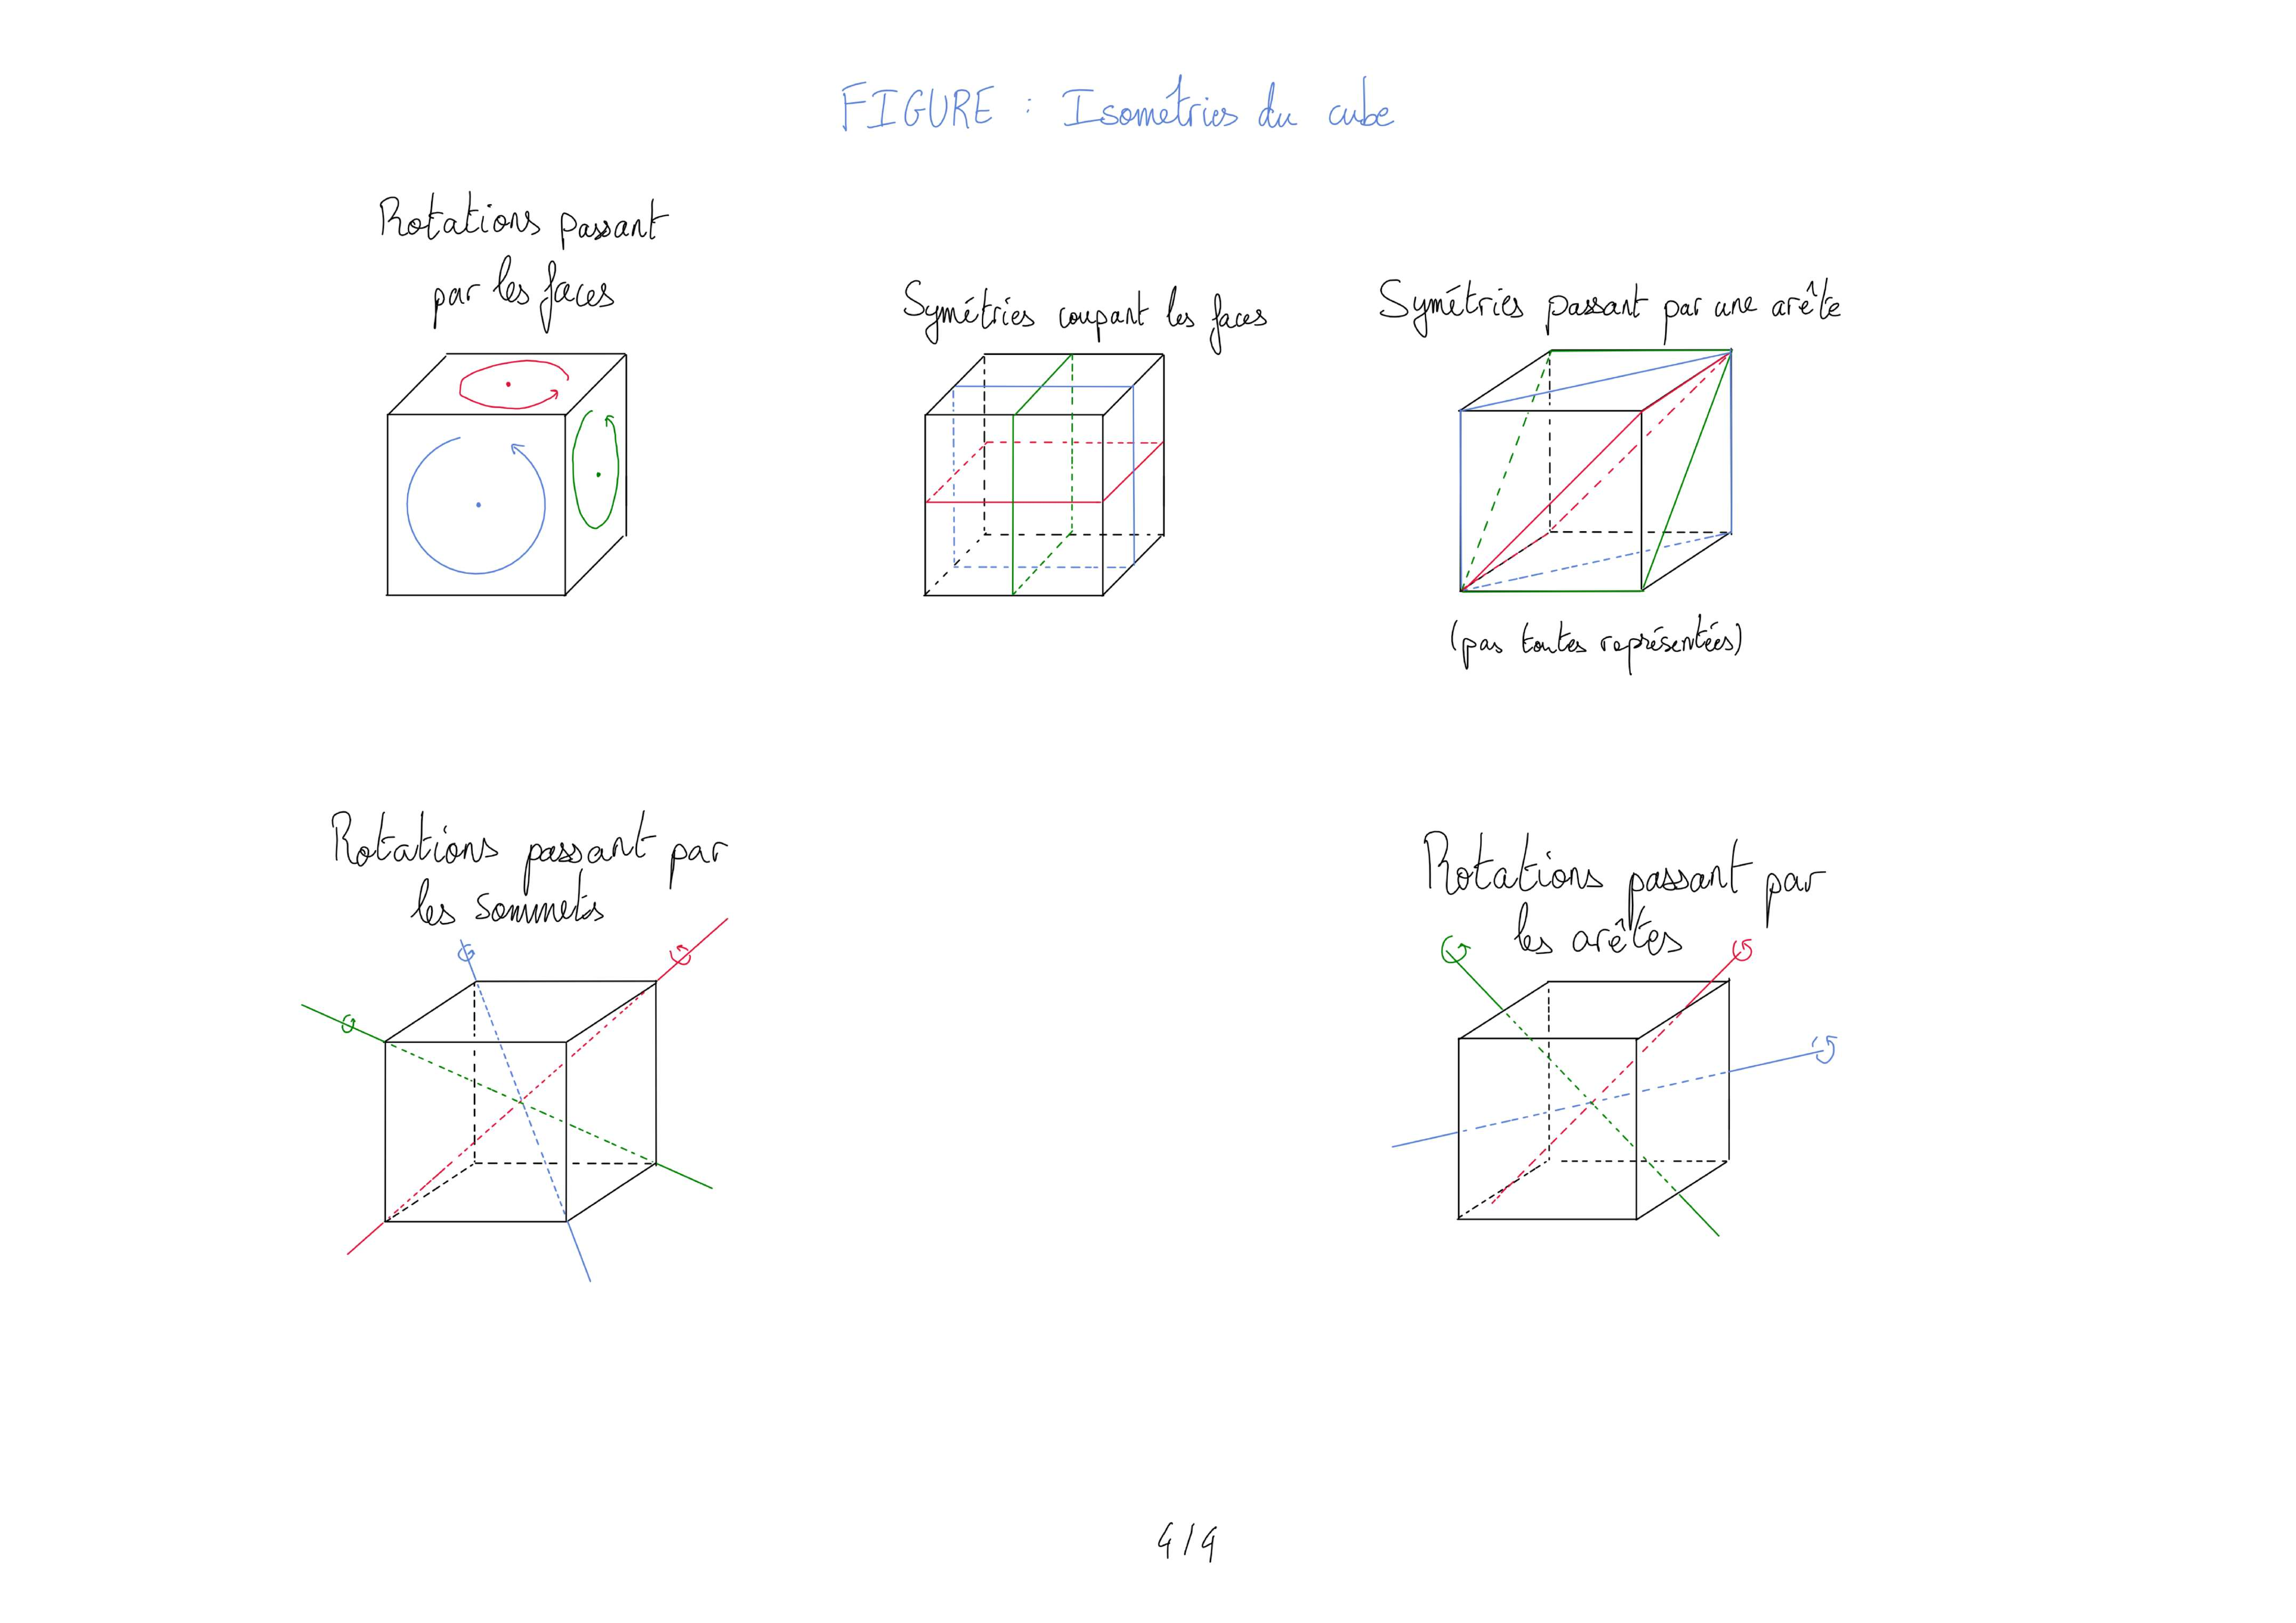
\includegraphics[trim={0 0 0 0},clip,width=1\linewidth]{img/101.pdf}
\end{figure}


\chapter*{105 : Groupe des permutations d'un ensemble fini. Applications.}
\setcounter{definition}{0}
\section*{I. Permutations d'un ensemble fini}
\subsection*{A. Introduction}
\begin{definition}[\textnormal{[R] 37}]
	Soit $E$ un ensemble. On note $\mathfrak{S}(E)$
	l'ensemble des bijections de $E$ dans $E$. On l'appelle \emph{groupe symétrique} de $E$.
	On notera plus simplement $\mathfrak{S}_n = \mathfrak{S}(\llbracket 1, n\rrbracket)$.
	On appelle \emph{permutation} de $E$ un élément de $\mathfrak{S}(E)$.
\end{definition}

\begin{proposition}
	$\mathfrak{S}(E)$ est un groupe pour la composition, de neutre l'identité de $E$.
\end{proposition}

\begin{proposition}[\textnormal{[R] 39}]
	Si $E$ et $F$ sont deux ensembles équipotents, alors $\mathfrak{S}(E)$ et $\mathfrak{S}(F)$ sont isomorphes (en tant que groupes).
\end{proposition}

\begin{proposition}[\textnormal{[R] 39}]
	Pour $n\geq 3$, $\mathfrak{S}_3$ n'est pas commutatif.
\end{proposition}

Dans toute la suite, on étudiera $\mathfrak{S}_n$ pour $n\geq 3$.

\begin{proposition}[\textnormal{[R] 40}]
	$\#\mathfrak{S}_n = n!$
\end{proposition}

\begin{notation*}[\textnormal{[U] 41}]
	Soit $\sigma\in\mathfrak{S}_n$. On représentera $\sigma$ par la matrice $2\times n$ :
	\begin{align*}
		\sigma = \left(\begin{smallmatrix} 
			1 & 2 & \cdots & n\\
			\sigma(1) & \sigma(2) & \cdots & \sigma(n)
		\end{smallmatrix}\right)
	\end{align*}
\end{notation*}

\subsection*{B. Action naturelle de $\mathfrak{S}_n$ sur $\llbracket 1,n\rrbracket$, conséquences}

\begin{proposition}[\textnormal{[U] 41}]
		$\mathfrak{S}_n$ agit naturellement sur $\llbracket 1,n\rrbracket$ par $\sigma \cdot i = \sigma(i)$.
		Le morphisme associé est l'identité de $\mathfrak{S}_n$.
\end{proposition}

\begin{definition}[\textnormal{[U] 42}]
	On note $\Fix(\sigma)$ l'ensemble des points fixes de $\sigma\in\mathfrak{S}_n$.
	Son complémentaire dans $\llbracket 1,n\rrbracket$ est appelé \emph{support} de $\sigma$, et est noté $\Supp(\sigma)$.
\end{definition}

\begin{proposition}[\textnormal{[U] 43}]
	Soit $\sigma \in \mathfrak{S}_n$. Le sous-groupe $\langle\sigma\rangle$ agit sur $\llbracket 1,n\rrbracket$ par restriction
	de l'action de $\mathfrak{S}_n$. Les orbites de cette action sont appelées \emph{$\sigma$-orbites}.
	La réunion des $\sigma$-orbites ponctuelles est $\Fix(\sigma)$. Les $\sigma$-orbites non ponctuelles partitionnent $\Supp(\sigma)$.
\end{proposition}

\begin{example}
	Soit $\sigma = \left(\begin{smallmatrix} 
			1 & 2 & 3 & 4 & 5 \\
			2 & 1 & 3 & 5 & 4
		\end{smallmatrix}\right)$.
	On a $\Supp(\sigma)=\left\{1,2\right\}\sqcup \left\{4,5\right\}=\langle\sigma\rangle\cdot \left\{1\right\}\sqcup \langle\sigma\rangle\cdot\left\{4\right\}$.
\end{example}

\begin{definition}[\textnormal{[U] 43}]
	Un \emph{$k$-cycle} ($2\leq k \leq n$) est une permutation n'ayant qu'une seule $\sigma$-orbite non ponctuelle $\left\{i_1,\dots,i_k\right\}$.
	On la note $\sigma = (i_1,\dots,i_k)$ pour signifier que 
	$\forall j\notin \left\{i_1,\dots,i_k\right\}$, $\sigma(j)=j$ et $\sigma(i_j)=i_{j+1}$ en regardant les indices modulo $k$.

	Un $2$-cycle est appelé \emph{transposition}.
\end{definition}

\begin{proposition}[\textnormal{[U] 43}]
	$(i_1,i_2,\dots,i_k) = (i_2,i_3,\dots,i_k,i_1)=\dots=(i_k,i_1,i_2,\dots,i_{k-1})$
\end{proposition}

\begin{proposition}
	Un $k$-cycle est d'ordre $k$.
\end{proposition}

\subsection*{C. Décomposition d'une permutation, conséquences}

\begin{proposition}[\textnormal{[U] 42}]
	Deux permutations à supports disjoints commutent.
\end{proposition}

\begin{theorem}[\textnormal{[U] 43}]
	Toute permutation se décompose de manière unique (à l'ordre des facteurs près) comme produit de cycles à supports disjoints.
\end{theorem}

\begin{algorithm}[\textnormal{[U] 43}]
	Pour trouver une telle décomposition, il suffit de trouver les $r$-orbites.
	\begin{enumerate}
		\item On calcule $\sigma(1), \sigma^2(1),\dots$ justqu'à trouver $\sigma^{k_1}(1)=1$ (NB : $k_1\leq n$) ;
		\item On pose $i_2 = \min \llbracket 1,n\rrbracket \setminus (\langle\sigma\rangle\cdot\left\{1\right\})$, et de même on calcule $\sigma(i_2),\sigma^2(i_2),\dots$ jusqu'à trouver $\sigma^{k_2}(i_2)=i_2$ ;
		\item On itère jusqu'à épuiser $\llbracket 1,n\rrbracket$.
	\end{enumerate}
	On a alors $\sigma = (1,\sigma(1),\dots,\sigma^{k_1-1}(1))\circ (i_2, \sigma(i_2),\dots,\sigma^{k_2-1}(i_2))\circ \dots \circ(i_j, \sigma(i_j),\dots,\sigma^{k_j-1}(i_j))$
\end{algorithm}

\begin{example}
	$\sigma = \left(\begin{smallmatrix} 
			1 & 2 & 3 & 4 & 5 & 6 \\
			3 & 2 & 4 & 1 & 6 & 5
		\end{smallmatrix}\right) = (1,3,4)(5,6)$
\end{example}

\begin{proposition}[\textnormal{[R] 44}]
		$(i_1,\dots,i_k) = (i_1,i_2)(i_2,i_3)\dots(i_{k-1},i_k)$
\end{proposition}
\begin{corollary}[\textnormal{[R] 44}]
	Les transpositions engendrent $\mathfrak{S}_n$.
\end{corollary}
\begin{proposition}[\textnormal{[R] 45}]
	$\mathfrak{S}_n = \langle(i,i+1),\, 1\leq i\leq n\rangle = \langle (1,i), \, 2\leq i \leq n\rangle = \langle(1,2),\, (1,2,\dots, n) \rangle$
\end{proposition}

\begin{definition}[\textnormal{[U] 45}]
	On appelle \emph{type} de $\sigma\in\mathfrak{S}_n$ la liste croissante des cardinaux des $\sigma$-orbites.
\end{definition}

\begin{example}
	Le type de $(1,2,5)(3,4)(7,8)\in\mathfrak{S}_8$ est la liste $\left[1,2,2,3\right]$.
\end{example}

\begin{proposition}[\textnormal{[U] 46}]
	Deux permutations sont conjuguées dans $\mathfrak{S}_n$ si, et seulement si, elles ont le même type.
	Cela décrit donc les classes de conjugaison de $\mathfrak{S}_n$.
\end{proposition}

\begin{proposition}[\textnormal{[U] 45}]
	Si $\sigma$ est du type $\left[l_1,\dots,l_k\right]$, alors $\ord(\sigma) = l_1 \vee \dots \vee l_k$.
\end{proposition}

\subsection*{D. Signature dune permutation, groupe alterné}

\begin{proposition}[\textnormal{[R] 47}]
	Il existe un unique morphisme $\varepsilon\,\colon \mathfrak{S}_n \to \left\{\pm 1\right\}$ qui envoie
	les transpositions sur $-1$. On appelle \emph{signature} de $\sigma$ la quantité $\varepsilon(\sigma)$.
\end{proposition}

\begin{corollary}
	La signature d'un $k$-cycle est $(-1)^{k+1}$.
\end{corollary}

\begin{proposition}[\textnormal{[R] 48}]
	$\forall\sigma\in\mathfrak{S}_n$, 
	$$\varepsilon(\sigma) = \prod_{1\leq i\leq j\leq n}\frac{\sigma(j) - \sigma(i)}{j-i}$$
	En particulier, la signature mesure le nombre d'inversions.
\end{proposition}

\begin{definition}[\textnormal{[R] 48}]
	On appelle \emph{$n$-ième groupe alterné} le sous-groupe $\mathcal{A}_n = \Ker(\varepsilon)$.
	C'est l'ensemble des permutations dîtes \emph{paires}.
\end{definition}

\begin{example}
	$\mathcal{A}_3 = \left\{\textnormal{id},\, (1,2,3),\, (1,3,2)\right\}$.
\end{example}

\begin{proposition}
	$\#\mathcal{A}_n = \frac{n!}{2}$
\end{proposition}

\begin{theorem}[\textnormal{[R] 49}]
	Pour $n\geq 3$, les $3$-cycles engendrent $\mathcal{A}_n$, et y sont conjugués.
\end{theorem}

\begin{theorem}[\textnormal{[R] 50}]
	Pour $n\geq 5$, $\mathcal{A}_n$ n'admet pas de sous-groupe distingué non trivial.
\end{theorem}

\section*{II. Quelques applications du groupe symétrique}
\subsection*{A. En géométrie : les isométries des polytopes}

\begin{theorem}[\textnormal{[R] 94}]
	L'ensemble des isométries du plan conservant un triangle équilatéral est un groupe isomorphe à $\mathfrak{S}_3$.
\end{theorem}

\begin{proposition}[\textnormal{[R] 82}]
	Soit $\mathcal{C}$ un cube. L'ensemble des isométries de l'espace conservant $\mathcal{C}$ est un groupe, noté $\Is(\mathcal{C})$.
	On note $\Is^+(\mathcal{C})$ le sous-groupe de $\Is(\mathcal{C})$ formé des rotations.
\end{proposition}

\begin{tcolorbox}[
    breakable, % Allows the theorem to split across pages
    colback=developpement, % The background color
    colframe=gray!0!black, % The frame color
    boxrule=0pt, % The frame thickness
    arc=1mm, % Sharp corners
	boxsep=0pt,
	left=0pt, right=0pt, top=0pt, bottom=0pt
]
\begin{theorem}[\textnormal{[R] 85}]
	\label{105dev1}
	$\Is^+(\mathcal{C}) \cong \mathfrak{S}_4$ et $\Is(\mathcal{C})\cong \mathfrak{S}_4\times \IZ/2\IZ$.
\end{theorem}
\end{tcolorbox}

\begin{theorem}[\textnormal{[R] 95}]
	En notant $\mathcal{T}$ le tétraèdre régulier, on a :
	$\Is(\mathcal{T})\cong \mathfrak{S}_4$ et $\Is^+(\mathcal{T})\cong \mathcal{A}_4$.
\end{theorem}

\subsection*{Chez les (actions de) groupes}
\begin{theorem}[de Cayley - \textnormal{[R] 53}]
	Tout groupe fini d'ordre $n$ est isomorphe à un sous-groupe de $\mathfrak{S}_n$.
\end{theorem}
\begin{proposition}
	Comme pout tout corps (commutatif) $K$, $\mathfrak{S}_n\actson GL_n(K)$, tout groupe de garde $n$ 
	est isomorphe à un sous-groupe de $GL_n(K)$.
\end{proposition}

\begin{example}
	Soit $D_{2\times 4}$ le groupe des isométries du carré. Comme $\#D_{2\times 4} = 8$, $D_{2\times 4}$ est isomorphe à un sous-groupe de $\mathfrak{S}_8$. Noton $\varphi$ un tel isomorphisme.
	Comme $D_{2\times 4} = \langle r, s\rangle$ où $\ord(r) = 4$, $\ord(s) = 2$ et $\ord(rs) = 2$, on a $\varepsilon\circ \varphi(s)=\varepsilon\circ \varphi(rs) = -1$, donc $\varepsilon\circ \varphi(r) = 1$.
\end{example}

\subsection*{C. Polynômes symétriques}
\begin{definition}[\textnormal{[R] 55}]
	Un \emph{polynôme symétrique} est un polynôme $P\in K[X_1,\dots,X_n]$
	tel que $\forall\sigma\in\mathfrak{S}_n$, $P(X_{\sigma(1)},\dots,X_{\sigma(n)}) = P(X_1,\dots,X_n)$.
\end{definition}

\begin{definition}[\textnormal{[R] 55}]
	Les \emph{polynômes symétriques élémentaires} sont les 
	\begin{align*}
		\Sigma_{k,n} = \sum_{1\leq i_1\leq\dots\leq i_k\leq n} X_{i_1}\dots X_{i_k}\in K[X_1,\dots,X_n]
	\end{align*}
\end{definition}

\begin{theorem}[ADMIS - \textnormal{[R] 55}]
	Pour tout polynôme symétrique $P\in K[X_1,\dots,X_n]$, il
	existe un unique polynôme $Q\in K[X_1,\dots,X_n]$ tel que 
	$P(X_1,\dots,X_n) = Q(\Sigma_{1,n},\dots,\Sigma_{n,n})$.
\end{theorem}

\subsection*{D. En algèbre (multi-)linéaire}
Dans ce paragraphe, $E$ est un $\mathbb{K}$-espace vectoriel de dimension finie $n$.
On fixe une base $\mathcal{B} = (e_1,\dots,e_n)$ de $E$.
\begin{definition}[\textnormal{[R] 545}]
	Une \emph{forme $k$-linéaire} sur $E$ est une application $\varphi \,\colon E^k\to \mathbb{K}$ telle que pour tout $i\in\llbracket 1,n\rrbracket$, pour tout $(x_1,\dots, x_k)\in E^k$,
	$\varphi(x_1,\dots,x_{i-1}, \cdot, x_{i+1}, \dots, x_k)$ est linéaire.

	On note $\bigotimes^k E^*$ l'ensemble des formes $k$-linéaires sur $E$.
\end{definition}

\begin{proposition}[\textnormal{[R] 546}]
	$\left(e_{i_1}^*\otimes\dots\otimes e_{i_k}^*\right)_{1\leq i_1<\dots < i_k\leq n}$ est une base de $\bigotimes^kE^*$,
	où pour $(x_1,\dots, x_k)\in E^k$, $e_{i_1}^*\otimes\dots\otimes e_{i_k}^*(x_1,\dots, x_k) = e_{i_1}^*(x_1)\dots e_{i_k}^*(x_k)$.
\end{proposition}

\begin{definition}[\textnormal{[R] 546}]
	Une forme $k$-linéaire \emph{alternée} est une forme $k$-linéaire $\varphi\in\bigotimes^kE^*$
	telle que $\forall\sigma\in\mathfrak{S}_k$, $\forall(x_1,\dots, x_k)\in E^k$, $\varphi(x_{\sigma(1)},\dots, x_{\sigma(k)}) = \varepsilon(\sigma)\varphi(x_1,\dots, x_k)$.

	On note $\bigwedge^k E^*$ l'espace des formes $k$-linéaires alternées sur $E$.
\end{definition}

\begin{proposition}
	$\left(e_{i_1}^*\wedge \dots \wedge e_{i_k}^*\right)_{1\leq i_1 < \dots < i_k\leq n}$ est une base de $\bigwedge^kE^*$, où pour $(x_1,\dots,x_k)\in E^k$,
	$e_{i_1}^*\wedge \dots \wedge e_{i_k}^*(x_1,\dots,x_k) = \sum_{\sigma\in\mathfrak{S}_k} \varepsilon(\sigma) e_{i_1}^*(x_{\sigma(1)}) \dots e_{i_k}^*(x_{\sigma(k)})$.
\end{proposition}

\begin{corollary}
	On a $\dim\left(\bigwedge^kE^*\right) = {n \choose k}$.
\end{corollary}

\begin{definition}
	On appelle \emph{déterminant dans la base $\mathcal{B}$} l'unique forme $n$-linéaire alternée $\det_{\mathcal{B}}$ sur $E$ vérifiant
	$\det_{\mathcal{B}}(\mathcal{B}) = 1$. (La fammille $\left(\det_{\mathcal{B}}\right)$ est une base de $\bigwedge^n E^*$.)
\end{definition}

\begin{proposition}[\textnormal{[R] 547}]
	$\forall(x_1,\dots, x_n)\in E^n$, $\det_{\mathcal{B}}(x_1,\dots,x_n) = \sum_{\sigma\in\mathfrak{S}_n} \varepsilon(\sigma)e_1^*(x_{\sigma(1)})\dots e_n^*(x_{\sigma(n)})$.
\end{proposition}

\subsection*{E. Résultats en probabilités}

\begin{definition}[\textnormal{[R] 51}]
	On appelle \emph{dérangement} une permutation sans point fixes.
\end{definition}

\begin{proposition}
	Notons $d_n$ le nombre de dérangements de $\llbracket 1,n\rrbracket$.
	Alors $d_n = n!\sum_{k=0}^{n}\frac{(-1)^k}{k!}$. En particulier, la probabilité
	de choisir un dérangement en tiant au hasard une permutation de $\llbracket 1,n\rrbracket$ tend vers $\frac{1}{e}$ quand $n\to +\infty$.
\end{proposition}

\begin{proposition}[\textnormal{[C]}]
	Soit $X$ la variable aléatoire qui compte le nombre de points fixes d'une permutation aléatoirement choisie dans $\mathfrak{S}_n$.
	Alors $\mathbb{E}[X] = \mathbb{V}[X] = 1$.
\end{proposition}

\subsection*{F. Groupes simples d'ordre 60}
Dans ce paragraphe, on se donne $p$ premier, et on note $\#G = p^{\alpha}m$, $m\wedge p = 1$.

\begin{definition}[\textnormal{[U] 85}]
	Un \emph{$p$-Sylow} de $G$ est un sous-groupe de $G$ de cardinal $p^{\alpha}$.
\end{definition}

\begin{notation*}
	$\Syl_p(G)$ désigne l'ensemble des $p$-Sylow de $G$, et $n_p =\#\Syl_p(G)$.
\end{notation*}

\begin{theorem}[de Sylow - \textnormal{[U] 87}]
	Soit $G$ un groupe d'ordre $p^{\alpha}m$, $p$ premier et $m\wedge p = 1$.
	\begin{enumerate}
		\item $\Syl_p(G)\neq \emptyset$
		\item $G$ agit transitivement sur $\Syl_p(G)$ par conjugaison
		\item $n_p \equiv 1\,[p]$ (donc $n_p\mid m$).
	\end{enumerate}
\end{theorem}

\begin{definition}
	On dit que $G$ est \emph{simple} si les seuls sous-groupes de $G$ distingués (\emph{i.e.} fixe par l'action par conjugaison de G) sont $\left\{1\right\}$ et $G$.
\end{definition}

\begin{tcolorbox}[
    breakable, % Allows the theorem to split across pages
    colback=developpement, % The background color
    colframe=gray!0!black, % The frame color
    boxrule=0pt, % The frame thickness
    arc=1mm, % Sharp corners
	boxsep=0pt,
	left=0pt, right=0pt, top=0pt, bottom=0pt
]
\begin{theorem}[\textnormal{[S] - 277}]
	\label{105dev2}
	Si $G$ est simple et d'ordre $60$, alors $G\cong \mathcal{A}_5$.
\end{theorem}
\end{tcolorbox}

\section*{Développements}
\begin{itemize}
	\item Développement 1 : Théorème \ref{105dev1}
	\item Développement 2 : Théorème \ref{105dev2}
\end{itemize}

\section*{Références}
\begin{itemize}
	\item[R] \emph{Mathématiques pour l'agrégation - Algèbre et géométrie}, Jean-Étienne Rombaldi, 2e édition
	\item[U] \emph{Théorie des groupes}, Félix Ulmer
	\item[S] \emph{Algèbre pour la licence 3}, Szpirglas
	\item[C] \emph{Carnets de voyage en Algébrie}, Caldero
\end{itemize}

\begin{figure}[!htb]
	\centering
	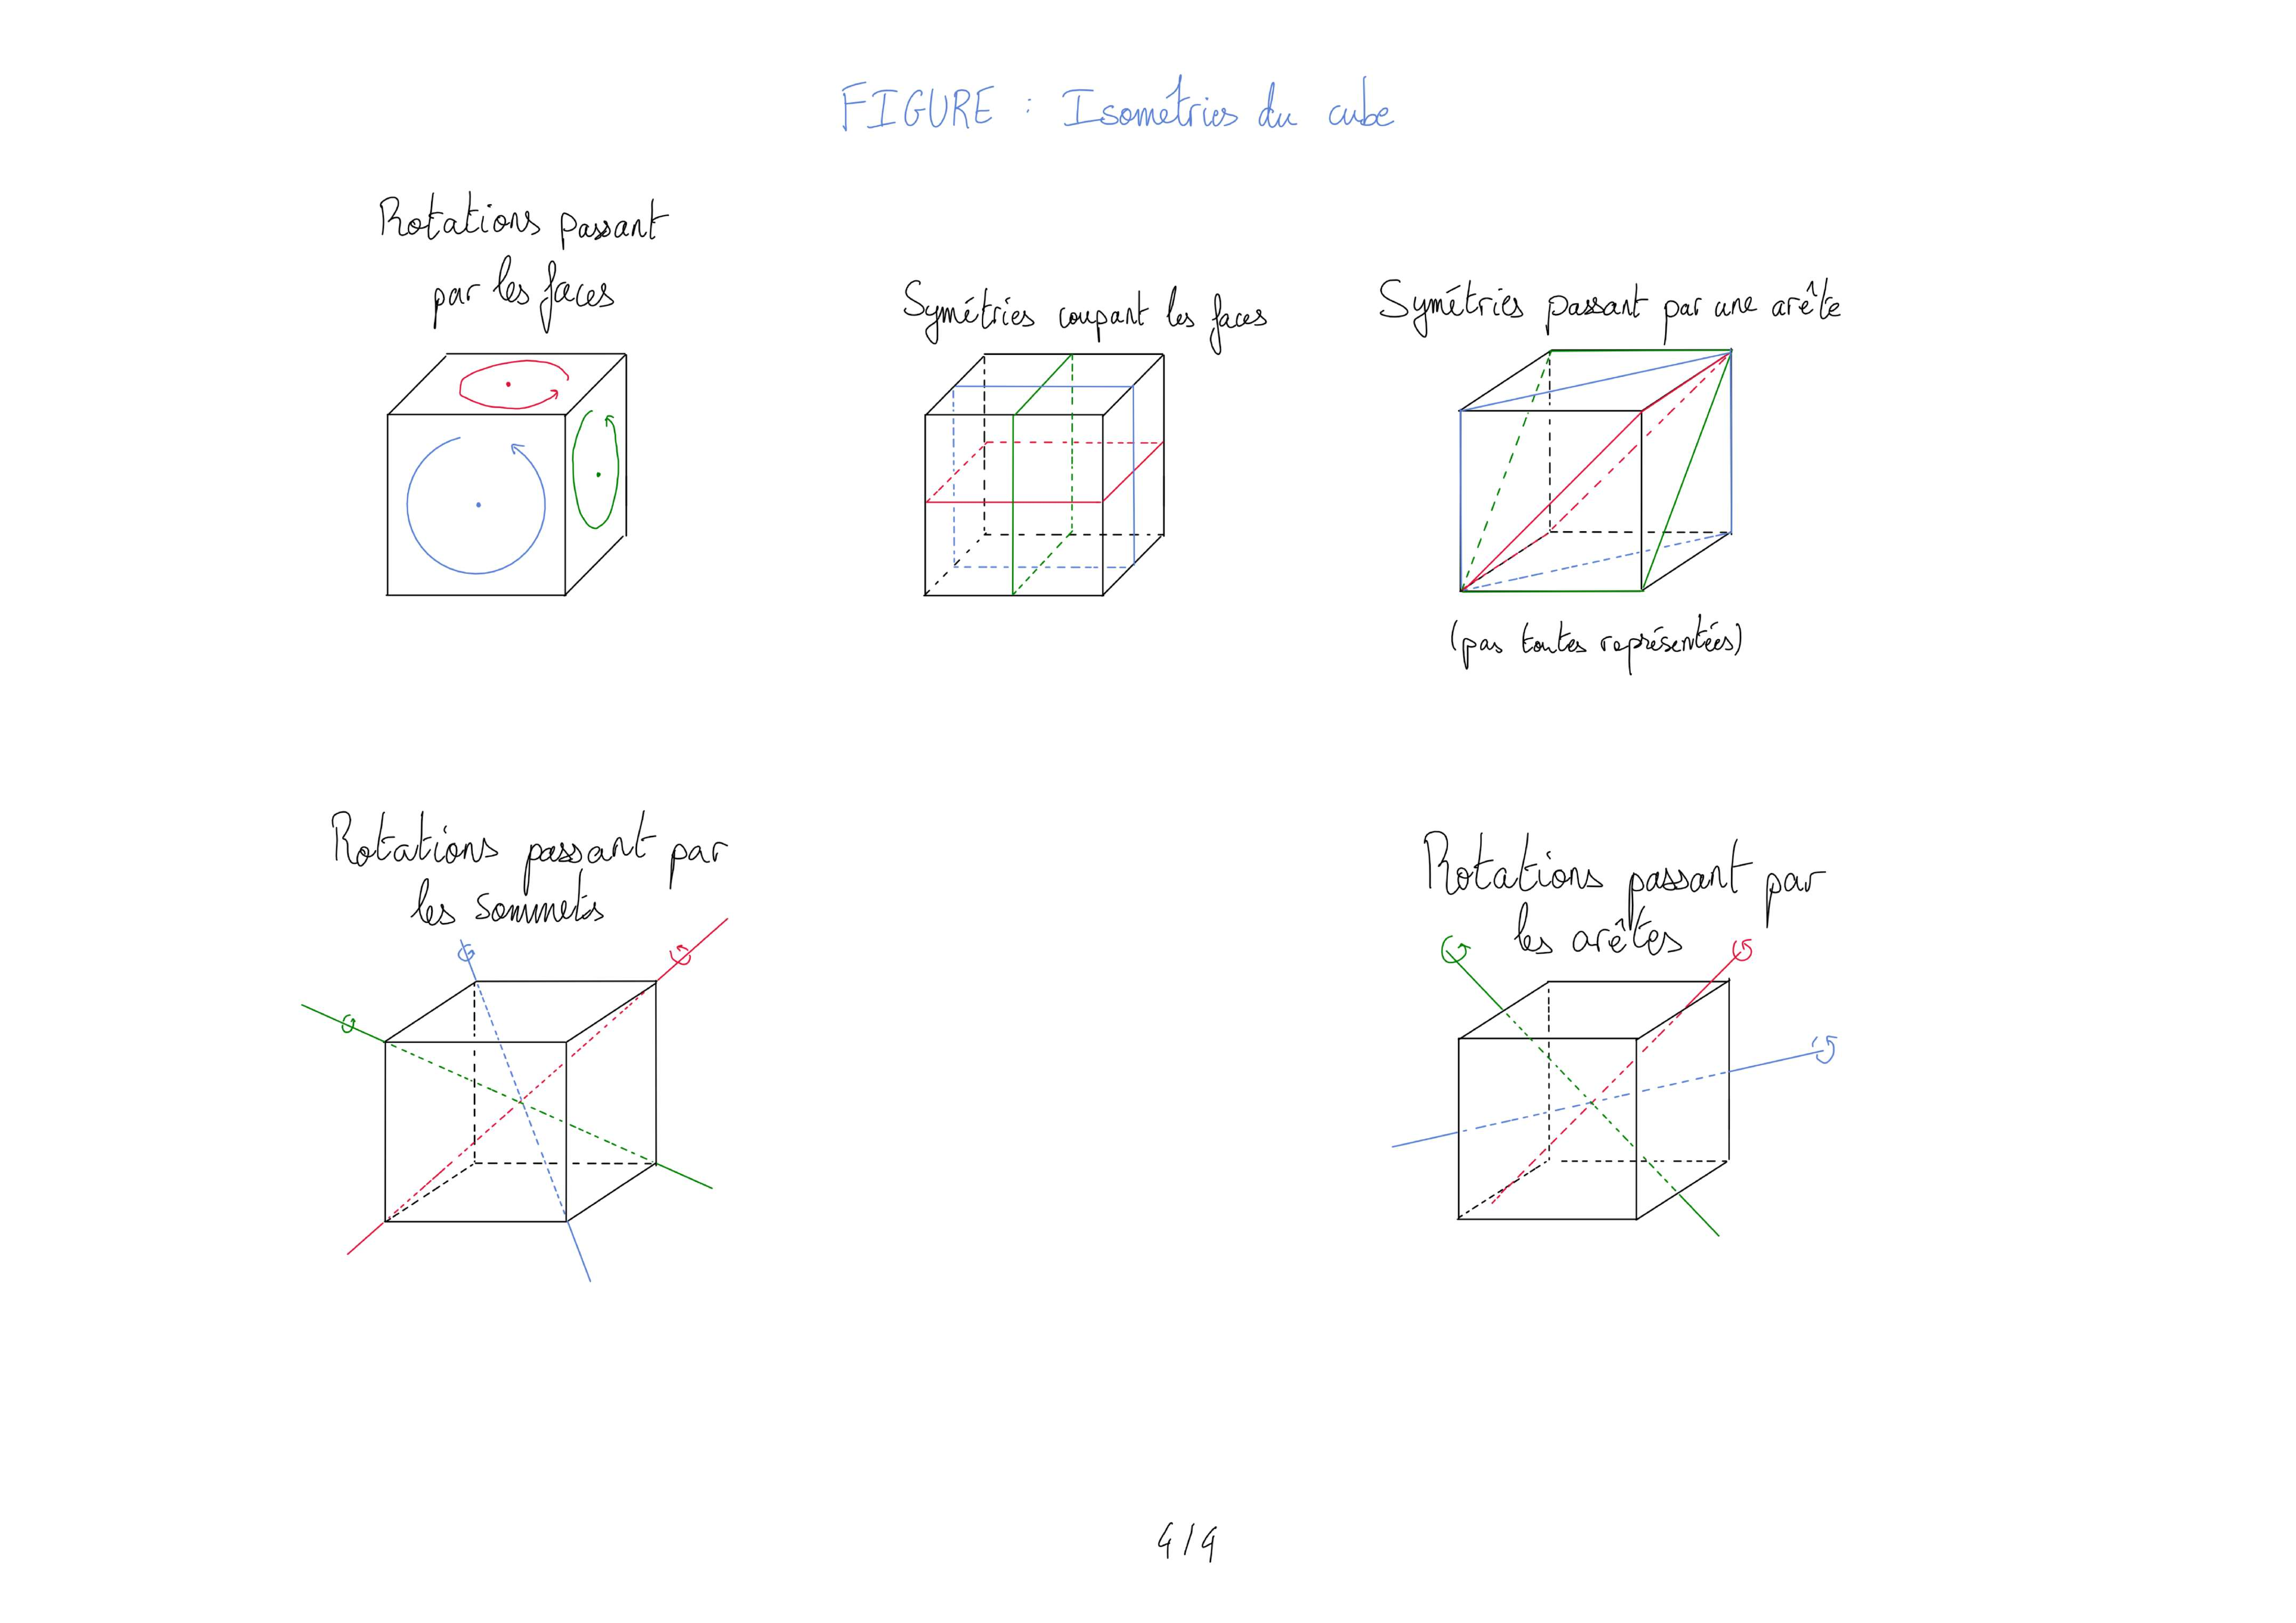
\includegraphics[trim={0 0 0 0},clip,width=1\linewidth]{img/101.pdf}
	\caption{Isométries du cube}
\end{figure}

\chapter*{106 : Groupe linéaire d'un espace vectoriel de dimension finie E, sous-groupes de $GL(E)$. Applications}
\setcounter{definition}{0}

Dans cette leçon, $K$ est un corps commutatif, et $E$ est un $K$-espace vectoriel de dimension finie $n\geq 1$.
\section*{I. Endomorphismes inversibles d'un espace vectoriel}
\subsection*{A. Introduction au groupe linéaire}
\begin{theorem}[\textnormal{[Rb] 139}]
	\begin{itemize}
		\item L'ensemble $\mathcal{L}(E)$ des endomorphismes de $E$ est un anneau pour $+$ et $\circ$, dont le groupe des inversibles est noté $GL(E)$, et est appelé \emph{groupe linéaire} de $E$.
		\item Similairement, l'ensemble $\M_n(K)$ des matrices carrées de taille $n\times n$ est un anneau pour $+$ et $\times$, dont le groupe des inversibles est noté $GL_n(K)$, appelé \emph{groupe linéaire d'ordre $n$ sur $K$}.
	\end{itemize}
\end{theorem}

\begin{remark}[\textnormal{[Rb] 140}]
	Étant donnée une base $\mathcal{B}$, l'application $u\mapsto \Mat_{\mathcal{B}}(u)$ induit un isomorphisme entre $GL(E)$ et $GL_n(K)$.
\end{remark}

\begin{definition}[\textnormal{[Rb] 141}]
	On note $SL(E)$ (resp. $SL_n(K)$) le noyau du morphisme $\det$ de $GL(E)$ (resp. $GL_n(K)$) dans $K^{\times}$.
	On l'appelle \emph{groupe spécial linéaire de $E$} (resp. \emph{groupe spécial linéaire d'ordre $n$ sur $K$}).
\end{definition}

\begin{theorem}[\textnormal{[Rb] 140}]
	Soit $u\in\mathcal{L}(E)$. Comme $\dim E < +\infty$, sont équivalentes :
	\begin{enumerate}
		\item $u\in GL(E)$
		\item {\begin{enumerate}
			\item $u$ est injectif
			\item $\Ker u = \left\{0\right\}$
			\item $\exists v\in \mathcal{L}(E)\,\colon v\circ u = \id_E$
		\end{enumerate}}
		\item {\begin{enumerate}
			\item $u$ est surjectif
			\item $\im u = E$
			\item $\exists v\in \mathcal{L}(E)\,\colon u\circ v = \id_E$
		\end{enumerate}}
		\item L'image par $u$ d'une base de $E$ est une base de $E$
		\item $\det(u) \neq 0$
	\end{enumerate}
\end{theorem}

\begin{remark}
	Un matrice $A$ est inversible si, et seulement si, ses colonnes forment une base de $K^n$, et si, et seulement si, ses lignes forment une base de $K^n$.
\end{remark}

\begin{definition}
	On dit que $u\in\mathcal{L}(E)$ est une \emph{homothétie de rapport $\lambda\in K^{\times}$} si $\forall x\in E$, $u(x) = \lambda x$.
\end{definition}

\begin{proposition}
	Une homothétie de rapport $\lambda\in K^{\times}$ est inversible, d'inverse l'homothétie de rapport $1/\lambda$.
\end{proposition}

\begin{proposition}[\textnormal{[Rb] e168}]
	Les homothéties sont les seuls endomorphismes à stabiliser toute droite.
\end{proposition}

\subsection*{B. Opérations élémentaires}
Soit $A\in\M_n(K)$. On note $L_1, \dots, L_p$ les lignes de $A$, et $C_1,\dots,C_n$ ses colonnes.
\begin{definition}[\textnormal{[Bu] 315-317}]
	Soient $\alpha \in K^{\times}$, $(i,j)\in\llbracket 1,n\rrbracket^2$ tel que $i\neq j$ et $\sigma\in\mathfrak{S}_n$. On définit les matrices suivantes :
	\begin{itemize}
		\item Matrice de \emph{dilatation} $D_i(\alpha) = \diag(1,\dots, 1, \alpha,1,\dots, 1)\in GL_n(K)$ ($\alpha$ est à la $i$-ième position)
		\item Matrice de \emph{transvection} $T_{i,j}(\alpha) = I_n + \alpha E_{i,j}\in GL_n(K)$
		\item Matrice de \emph{permutation} $P_{\sigma} = \left(\delta_{i,\sigma(j)}\right)_{1\leq i,j\leq n}\in GL_n(K)$
	\end{itemize}
\end{definition}

\begin{definition}
	On définit les \emph{opérations élémentaires} sur les colonnes :
	\begin{itemize}
		\item $C_i \longleftarrow \alpha C_i$ : on remplace $C_i$ par $\alpha C_i$
		\item $C_i \longleftarrow C_i + \alpha C_j$ : on remplace $C_i$ par $\alpha C_i+\alpha C_j$
		\item $C_i \longleftrightarrow C_j$ : on échange $C_i$ et $C_j$
	\end{itemize}
\end{definition}

\begin{theorem}[\textnormal{[Bu] 315-318}]
	On a les correspondances suivantes entre opérations élémentaires et multiplication matricielle :
	\begin{itemize}
		\item $D_i(\alpha)A\iff L_i \longleftarrow \alpha L_i$
		\item $T_{i,j}(\alpha)A\iff L_i \longleftarrow L_i \alpha L_j$
		\item $P_{(i,j)}A\iff L_i \longleftrightarrow L_j$
	\end{itemize}
	et 
	\begin{itemize}
		\item $A D_i(\alpha)\iff C_i \longleftarrow \alpha C_i$
		\item $AT_{i,j}(\alpha)\iff C_i \longleftarrow C_i \alpha C_j$
		\item $AP_{(i,j)}\iff C_i \longleftrightarrow C_j$
	\end{itemize}
\end{theorem}

\begin{proposition}
	$\sigma\mapsto P_{\sigma}$ est un morphisme de groupes injectif de $\mathfrak{S}_n$ dans $GL_n(K)$.
\end{proposition}

\section*{II. Structure de $GL(E)$, sous-groupe orthogonal}
\subsection*{A. Structure de groupe}

\begin{theorem}[Pivot de Gauss - \textnormal{[Rb] 191}]
	Pour toute matrice de rang $r$, il existe une suite d'opérations élémentaires qui transforme cette matrice en la matrice $J_{n,r} = \diag(I_r, O_{n-r})$.
	Plus précisément, si $\rg A = n$, alors il existe $\sigma\in\mathfrak{S}_n$ et des matrices de transvection $T_1, \dots, T_p$ telles que $A = P_{\sigma}T_1\dots T_p D_{\alpha}$ où $D_{\alpha}$ est la matrice de dilatation $D_{\alpha}$ de rapport $\alpha = \det A$.
\end{theorem}

\begin{corollary}[\textnormal{[Rb] 154, 153}]
	\begin{itemize}
		\item Les matrices de transvection et de dilatation engendrent $GL_n(K)$ ;
		\item Les matrices de transvection engendrent $SL_n(K)$.
	\end{itemize}
\end{corollary}

\begin{corollary}[\textnormal{[Rb] 141}]
	$GL(E) / SL(E) \cong K^{\times}$
\end{corollary}

\begin{corollary}[\textnormal{[Rb] 141}]
	\begin{itemize}
		\item $Z(GL(E)) = K^{\times}\id_E$ (c'est l'ensemble des homothéties) ;
		\item $Z(SL(E)) = \mathbb{U}_n(K)\id_E$, où $\mathbb{U}_n(K)  \left\{\lambda\in K^{\times} \mid \lambda^n = 1\right\}$.
	\end{itemize}
\end{corollary}

\subsection*{B. Le groupe spécial orthogonal}
Soit $q$ une forme quadratique sur $E$, de forme polaire $\varphi$. Supposons $\car K \neq 2$.

\begin{definition}[\textnormal{[P] 123-124}]
	\begin{itemize}
		\item Le \emph{groupe orthogonal} de $(E,q)$ est $O(q) = \left\{u\in\mathcal{L}(E)\mid q\circ u = q\right\}$
		\item Le \emph{groupe spécial orthogonal} de $(E,q)$ est $SO(q) = \left\{u\in O(q)\mid \det u = 1\right\}$
		\item Lorsque $\varphi$ est le produit scalaire canonique relativement à une base donnée, on note $O(E)=O(q)=\left\{u\in\mathcal{L}(E)\mid {}^tu\circ u = \id_E\right\}$ et $SO(E)=SO(q)=\left\{u\in O(E)\mid \det u = 1\right\}$.
		\item On note également $O_n(K) = \left\{M\in\M_n(K)\mid {}^tMM=I_n\right\}$ et $SO_n(K)  \left\{M\in O_n(K)\mid \det M = 1\right\}$.
	\end{itemize}
\end{definition}

\begin{proposition}[\textnormal{[Rb] 722}]
	Si $\mathcal{B}$ est une base orthonormale de $E$, alors $u\in O(E)\iff \Mat_{\mathcal{B}}(u)\in O_n(K)$.
\end{proposition}

\begin{theorem}[de réduction des isométries - \textnormal{[Rb] 727}]
	Soit $u\in O(\IRn)$. Il existe une base orthonormale $\mathcal{B}$ de $\IRn$ telle que $\Mat_{\mathcal{B}}(u)=\diag(R(\theta_1),\dots,R(\theta_r),\varepsilon_1,\dots,\varepsilon_p)$
	où $R(\theta_i) = \begin{pmatrix}
		\cos \theta_i & -\sin \theta_i \\
		\sin \theta_i & \cos \theta_i
	\end{pmatrix}$ et $\varepsilon_i = \pm 1$.
\end{theorem}

\begin{remark}[\textnormal{[P] 146}]
	$SO_2(\IR) = \left\{R(\theta)\mid \theta\in\IR\right\}\cong \IR/2\pi\IZ$.
\end{remark}

\begin{tcolorbox}[
    breakable, % Allows the theorem to split across pages
    colback=developpement, % The background color
    colframe=gray!0!black, % The frame color
    boxrule=0pt, % The frame thickness
    arc=1mm, % Sharp corners
	boxsep=0pt,
	left=0pt, right=0pt, top=0pt, bottom=0pt
]
\begin{theorem}[\textnormal{[C] 50}]
	\label{106dev1}
	Soient $p$ premier, $r\geq 1$ et $q = p^r$.
	\begin{align*}
		SO_2(\IF_q) \cong \begin{cases}
			\IZ/(q-1)\IZ\quad\text{si $-1$ est un carré mod $q$} \\
			\IZ/(q+1)\IZ\quad \text{sinon}
		\end{cases}
	\end{align*}
\end{theorem}
\end{tcolorbox}

\begin{definition}[\textnormal{[P] 125}]
	Soit $u\in O(q)$ telle que $u^2 = \id_E$.
	
	On dit que $u$ est une \emph{réflexion} si $\dim(\Ker(u+\id_E)) = 1$, \emph{i.e.} si $u$ est une symétrie par rapport à un hyperplan.
	
	On dit que $u$ est une \emph{renversement} si $\dim(\Ker(u+\id_E)) = 2$, \emph{i.e.} si $u$ est une symétrie par rapport à un plan.
\end{definition}


\begin{tcolorbox}[
    breakable, % Allows the theorem to split across pages
    colback=developpement, % The background color
    colframe=gray!0!black, % The frame color
    boxrule=0pt, % The frame thickness
    arc=1mm, % Sharp corners
	boxsep=0pt,
	left=0pt, right=0pt, top=0pt, bottom=0pt
]
On suppose désormais que $E$ est un $\IR$-espace vectoriel de dimension finie $n\geq 1$, et que $q$ est définie positive.
\begin{theorem}[\textnormal{[P] 143}]
	\label{106dev21}
	Tout élément de $O(q)$ est produit d'au plus $n$ réflexions.
\end{theorem}
\begin{lemma}
	\label{106dev22}
	Si $n\geq 3$, alors pour toutes réflexions $\tau_1$ et $\tau_2$, il existe deux renversements $\sigma_1$ et $\sigma_2$ tels que $\tau_1\tau_2 = \sigma_1\sigma_2$.
\end{lemma}
\begin{theorem}
	\label{106dev23}
	Pour $n\geq 3$, tout élément de $SO(q)$ est produit d'au plus $n$ renversements.
\end{theorem}
\end{tcolorbox}

\begin{remark}
	Ces théorèmes restent vrais si $E$ est un espace vectoriel de dimension finie sur un corps $K$ de caractéristique $\neq 2$, et si $q$ est non dégénérée (Cartan, Dieudonné).
\end{remark}

\section*{III. Topologie dans $GL(E)$}
Dans ce paragraphe, $K$ désigne $\IR$ ou $\IC$.

\begin{proposition}[\textnormal{[Rb] 160-161}]
	$GL(E)$ est ouvert dans $(\mathcal{L}(E), \vertiii\cdot)$ et $u\mapsto u^{-1}$ est continue.
\end{proposition}

\begin{proposition}
	\begin{itemize}
		\item $GL_n(\IC)$ et $SL_n(K)$ sont connexes ;
		\item $GL_n(\IR)$ a deux composantes connexes.
	\end{itemize}
\end{proposition}

\begin{proposition}
	$O_n(\IR)$ et $SO_n(\IR)$ sont compacts.
\end{proposition}

\begin{theorem}[Décomposition polaire - \textnormal{[Rb] 740}]
		\begin{align*}
			O_n(\IR)\times S_n^{++}(\IR) &\to GL_n(\IR) \\
			(H,S) &\mapsto HS
		\end{align*}
		est un homéomorphisme.
\end{theorem}

\section*{Développements}
\begin{itemize}
	\item Développement 1 : Théorème \ref{106dev1}
	\item Développement 2 : Théorème \ref{106dev21}, Lemme \ref{106dev22} et Théorème \ref{106dev23}
\end{itemize}

\section*{Références}
\begin{itemize}
	\item[Rb] \emph{Mathématiques pour l'agrégation - Algèbre et géométrie}, Jean-Étienne Rombaldi, 2e édition
	\item[P] \emph{Cours d'algèbre}, Perrin
	\item[B] \emph{Algèbre et géométrie: CAPES et Agrégation}, Pierre Burg
	\item[C] \emph{Nouvelles histoires hédonistes de groupes et géométries}, P. Caldero, J. Germoni
\end{itemize}


\chapter*{120 : Anneaux $\IZnZ$. Applications.}
Dans toute la leçon, $n\in\IN\setminus\left\{0,1\right\}$ et $p$ est un nombre premier.
\setcounter{definition}{0}
\section*{I. L'anneau $\IZnZ$}
\subsection*{A. Rappels d'arithmétique des entiers}
\begin{theorem}[division euclidienne - \textnormal{[R] 279}]
	$\forall (a,b)\in\IZ^2,\,\exists ! (q,r)\in\IZ^2 \,\colon$
	\begin{align*}
		\begin{cases}
			a=bq+r \\
			0\leq r< |b|
		\end{cases}
	\end{align*}
\end{theorem}

\begin{definition}[\textnormal{[R] 279}]
	Soit $(a,b)\in\IZ^2$. On dit que $a$ est \emph{congru à} $b$ modulo $n$,
	et on note $a\equiv b \, [n]$ si $n$ divise $b-a$.
\end{definition}

\begin{proposition}[\textnormal{[R] 280}]
	Soit $(a,b,c,d)\in\IZ^4$ tel que $a\equiv b\,[n]$ et $c\equiv d\,[n]$.
	Alors $a+c\equiv b+d\,[n]$ et $ac\equiv bd \,[n]$.
\end{proposition}

\subsection*{B. Construction}
\begin{lemma}
	Tout idéal de $\IZ$ est principal, et admet un unique générateur positif.
\end{lemma}

\begin{definition}[\textnormal{[R] 280}]
	Le quotient de l'anneau $(\IZ, +,\times)$ par son idéal $n\IZ$ est l'anneau noté $\IZnZ$. On note $\overline{a}$ l'image de $a\in\IZ$ dans $\IZnZ$.
\end{definition}

\begin{remark}
	$\overline{a} = \overline{b} \iff a\equiv b\,[n]$
\end{remark}

\begin{proposition}[\textnormal{[R] 280}]
	$\IZnZ = \left\{\overline{0},\overline{1},\dots,\overline{n-1}\right\}$, et les lois sont données par Prop 3 et Rq 6.
\end{proposition}

\begin{example}
	$\IZ/3\IZ = \left\{\overline{0},\overline{1},\overline{2}\right\} =\left\{\overline{9},\overline{64},\overline{-7}\right\}$,
	et on a $\overline{1}+\overline{2}=\overline{1+2}=\overline{3}=\overline{0}$, mais aussi $\overline{1}\times\overline{2} = \overline{1\times 2}=\overline{2}$.
\end{example}

\subsection*{C. Structure d'anneau}
\begin{proposition}[\textnormal{[R] 283}]
	L'ensemble des inversibles $\IZnZ$ est :
	$$\left(\IZnZ\right)^{\times} = \left\{\overline{k}\in\IZnZ\mid k\wedge n = 1\right\}$$

	L'ensemble des diviseurs de $O$ de $\IZnZ$ est :
	$$D_0\left(\IZnZ\right) = \IZnZ \setminus \left[\left(\IZnZ\right)^{\times}\cup \left\{0\right\}\right]$$
\end{proposition}

\begin{example}
	$\left(\IZ/8\IZ\right)^{\times} = \left\{\overline{1},\overline{3},\overline{5},\overline{7}\right\}$, et 
	$D_0\left(\IZ/8\IZ\right) = \left\{\overline{2},\overline{4},\overline{6}\right\}$.
\end{example}

\begin{proposition}[\textnormal{[R] 241 et 281}]
	Les idéaux propres de $\IZnZ$ sont les $d\IZnZ$ avec $d\mid n$, $d\notin \left\{1,n\right\}$.
	De plus, $\left(d\IZnZ, +\right)\cong \left(\IZ/\frac{n}{d}\IZ, +\right)$.
\end{proposition}

\begin{corollary}
	$\IZnZ$ est principal.
\end{corollary}

\begin{corollary}
	L'ensemble des générateurs de $\IZnZ$ est $\left(\IZnZ\right)^{\times}$.
\end{corollary}

\begin{example}
	Les idéaux propres de $\IZ/6\IZ$ sont $2\IZ/6\IZ$ et $3\IZ/6\IZ$, respectivement isomorphes à $\IZ/3\IZ$ et $\IZ/2\IZ$.
\end{example}

\begin{proposition}[\textnormal{[R] 295-282}]
	$\forall n,m\geq 2$, 
	$$\Hom_{gr}(\IZnZ, \IZ/m\IZ)\cong \IZ/(n\wedge m)\IZ,$$
	$$\Aut(\IZnZ)\cong \left(\IZnZ\right)^{\times},$$
	$$\Hom_{Ann}(\IZnZ, \IZ/m\IZ)\cong  \begin{cases}
		\left\{k\text{ mod } n \mapsto k \text{ mod } m\right\} \quad\text{si } m\mid n \\
		\emptyset\quad\text{sinon}
	\end{cases}$$
\end{proposition}

\subsection*{D. Le corps $\IZ/p\IZ$}
\begin{theorem}
	Les assertions suivantes sont équivalentes :
	\begin{enumerate}
		\item $\IZnZ$ est un corps ;
		\item $\IZnZ$ est intègre ;
		\item $n$ est premier.
	\end{enumerate}
\end{theorem}

\begin{corollary}[\textnormal{[R] 292}]
	$\left(\IZ/p\IZ\right)^{\times} \cong \IZ/(p-1)\IZ$.
\end{corollary}

\begin{cexample}
	C'est très faux pour $n$ non premier !
	$\left(\IZ/8\IZ\right)^{\times} = \left\{\overline{1},\overline{3},\overline{5},\overline{7}\right\}$ n'a même pas $7$ éléments !
\end{cexample}

\section*{II. Structure de $\left(\IZnZ\right)^{\times}$}
\subsection*{A. Préambule : le théorème des restes chinois}

\begin{tcolorbox}[
    breakable, % Allows the theorem to split across pages
    colback=developpement, % The background color
    colframe=gray!0!black, % The frame color
    boxrule=0pt, % The frame thickness
    arc=1mm, % Sharp corners
	boxsep=0pt,
	left=0pt, right=0pt, top=0pt, bottom=0pt
]
\begin{theorem}[des restes chinois - \textnormal{[R] 285}]
	\label{120dev1}
	Soit $(a_1,\dots, a_d)\in \left(\IN\setminus \left\{0,1\right\}\right)^d$.
	Les entiers, $a_1,\dots, a_d$ sont deux à deux premiers si, et seulement si, les anneaux 
	$\IZ/a_1\dots a_d\IZ$ et $\IZ/a_1\IZ \times \dots \times \IZ/a_d\IZ$ sont isomorphes.

	Le cas échéant, il existe $(u_1,\dots,u_d)\in\IZ^d$ tel que $\sum_{i=1}^{d} a_ib_i =1$, où 
	$b_i = \frac{a_1\dots a_d}{a_i}$. L'application :

	\begin{align*}
		\overline{\varphi} \,\colon \IZ/a_1\dots a_d\IZ &\to \IZ/a_1\IZ \times \dots \times \IZ/a_d\IZ \\
		x\,mod\,a_1\dots a_d &\mapsto (x\,mod\,a_1,\dots, x\, mod\, a_d)
	\end{align*}
	est un isomorphisme d'anneaux, de réciproque :
	\begin{align*}
		\overline{\varphi}^{-1}\,\colon (x_1\,mod\,a_1,\dots, x_d\, mod\, a_d) \mapsto \sum_{i=1}^{d} x_i a_i b_i\, mod\, a_1\dots a_d
	\end{align*}
\end{theorem}
\end{tcolorbox}

\subsection*{B. Fonction indicatrice d'Euler}
\begin{definition}[\textnormal{[R] 283}]
	\emph{L'indicatrice d'Euler} est :
	$\varphi\,\colon n \mapsto \#\left(\IZnZ\right)^{\times} = \#\left\{k\in\llbracket 1,n\rrbracket \mid k\wedge n = 1\right\}$.
\end{definition}

\begin{example}
	$\varphi(8) = 4$ d'après Exemple 10.
\end{example}

\begin{proposition}[\textnormal{[R] 288}]
	Si $a\wedge b=1$, alors $\varphi(ab)=\varphi(a)\varphi(b)$.
	Pour tout $\alpha \in \IN^*$, $\varphi(p^{\alpha}) = p^{\alpha - 1}(p-1)$.
\end{proposition}

\begin{corollary}[\textnormal{[R] 288}]
	Si $n=p_1^{\alpha_1}\dots p_r^{\alpha_r}$ est la décomposition de $n$ en produit de facteurs premiers,
	alors :
	$$\varphi(n) = \prod_{i=1}^{r} p^{\alpha_i - 1}(p-1) = n\prod_{i=1}^{r}\left(1 - \frac{1}{p_i}\right)$$
\end{corollary}

\begin{example}
	$\varphi(90) = \varphi(3^2)\varphi(2)\varphi(5) = 3(3-1)(2-1)(5-1) = 24$
\end{example}

\begin{theorem}[d'Euler - \textnormal{[R] 283}]
	Si $a\wedge n = 1$, alors $a^{\varphi(n)} \equiv 1\,[n]$.
\end{theorem}

\begin{theorem}[de Fermat - \textnormal{[R] 284}]
	Si $a\wedge p = 1$, alors $a^{p-1} = 1\, [p]$.
	De manière générale, $a^p\equiv a\,[p]$.
\end{theorem}

\begin{proposition}[\textnormal{[R] 284}]
	$$n = \sum_{d\mid n} \varphi(d)$$
\end{proposition}


\begin{tcolorbox}[
    breakable, % Allows the theorem to split across pages
    colback=developpement, % The background color
    colframe=gray!0!black, % The frame color
    boxrule=0pt, % The frame thickness
    arc=1mm, % Sharp corners
	boxsep=0pt,
	left=0pt, right=0pt, top=0pt, bottom=0pt
]
\begin{theorem}[\textnormal{[R] 292}]
	\label{120dev2}
	Si $p\geq 3$, alors $\forall \alpha \geq 1$, $\left(\IZ/p^{\alpha}\IZ\right)^{\times}$ est cyclique.
\end{theorem}
\end{tcolorbox}

\begin{theorem}[ADMIS - \textnormal{[R] 294}]
	$\left(\IZnZ\right)^{\times}$ est cyclique si, et seulement si, $n\in \left\{2,4,p^{\alpha}, 2p^{\alpha}\right\}$ avec $p\geq 3$ (premier) et $\alpha\geq 1$.
\end{theorem}

\section*{III. Applications}
\subsection*{A. Résolution de systèmes de congruence}
\begin{theorem}[\textnormal{[R] 290}]
	L'équation $ax\equiv b\,[n]$ d'inconnue $x\in\IZ$ admet des solutions si, et seulement si, $a\wedge n \mid b$.

	Le cas échéant, $S(ax\equiv b\,[n]) = \frac{b}{a\wedge n}x_0 + \frac{n}{a\wedge n}\IZ$, où $x_0$ est une solution particulière de l'équation.
\end{theorem}

\begin{remark}
	Le théorème des restes chinois permet de résoudre des systèmes de congruences.
\end{remark}


\begin{tcolorbox}[
    breakable, % Allows the theorem to split across pages
    colback=developpement, % The background color
    colframe=gray!0!black, % The frame color
    boxrule=0pt, % The frame thickness
    arc=1mm, % Sharp corners
	boxsep=0pt,
	left=0pt, right=0pt, top=0pt, bottom=0pt
]
\begin{example}[\textnormal{[R] 291}]
	\label{120dev12}
	$S\left(\begin{cases}
		x\equiv 2\,[4] \\
		x\equiv 3\,[5] \\
		x\equiv 1\,[9]
	\end{cases}\right) = 118 + 180\IZ$
\end{example}
\end{tcolorbox}

\begin{remark}[\textnormal{[R] 291}]
	$S\left(\begin{cases}
		x\equiv x_1\,[a_1] \\
		x\equiv x_2\,[a_2]
	\end{cases}\right) =\begin{cases}
		\emptyset\quad\text{si } a_1\wedge a_2 \nmid x_1-x_2 \\
		x_0 + (a_1\vee a_2)\IZ\quad\text{sinon}
	\end{cases}$
\end{remark}

\subsection*{B. Carrés de $\IZ/p\IZ$}
Soit $c\,\colon \overline{x}\in\IZ/p\IZ \mapsto \overline{x}^2$.
On s'intéresse à $\im c$.

\begin{proposition}
	Tous les éléments de $\IZ/2\IZ$ sont des carrés.
\end{proposition}
On supposera désormais $p\geq 3$.

\begin{proposition}[\textnormal{[R] 426}]
	Soit $l\,\colon \overline{x}\in\IZ/p\IZ \mapsto \overline{x}^{\frac{p-1}{2}}$.
	\begin{itemize}
		\item $\forall \overline{x}\in\IZ/p\IZ$, $c\circ l(\overline{x}) = l\circ c(\overline{x}) = \overline{1}$
		\item $\Ker c = \im l =\left\{\pm 1\right\}$ et $\im c = \Ker l$.
	\end{itemize}
\end{proposition}

\begin{corollary}
	Il y a $\frac{p+1}{2}$ carrés dans $\IZ/p\IZ$.
\end{corollary}

\begin{theorem}[de Wilson - \textnormal{[R] 325}]
	$n$ est premier $\iff (n-1)! \equiv -1\, [n]$
\end{theorem}

\begin{proposition}[\textnormal{[P] 75}]
	$-1$ est un carré modulo $p$ si, et seulement si, $p\equiv 1\,[4]$. Le cas échéant $-1\equiv (2\times 3\times\dots\times \frac{p-1}{2})^2\,[p]$.
\end{proposition}

\begin{theorem}[des deux carrés de Fermat - \textnormal{[P] 56}]
	$p$ s'écrit comme somme de deux carrés d'entiers si, et seulement si, $p=2$ ou $p \equiv 1\,[4]$.
\end{theorem}

\subsection*{C. Algorithme de chiffrement RSA}

\begin{algorithm}[\textnormal{[G] 37}]
	Alice veut envoyer à Bob un message représenté par un nombre 
entier $m$, en tout sécurité.
\begin{itemize}
	\item Bob choisit en secret deux nombres premiers distincts $p$ et $q$ et calcule leur produit $n=pq$.
	\item Il choisit ensuite un entier $c<\varphi(n)=(p-1)(q-1)$ premier à $\varphi(n)$.
	\item Il trouve ensuite un entier $d$ tel que $cd \equiv 1\,[\varphi(n)]$.
	\item La clé publique de Bob est $(n,c)$, qu'il donne à Alice, et sa clé privée est $(n,d)$, qu'il garde secrète.
	\item Alice envoie à Bob le message $m^c$ mod $n$.
	\item Pour décoder le message, Bob calcule $\left(m^c\right)^d\equiv m\,[n]$.
\end{itemize}
\end{algorithm}

\section*{Développements}
\begin{itemize}
	\item Développement 1 : Théorème \ref{120dev1} (restes chinois) et exemple \ref{120dev12}
	\item Développement 2 : Théorème \ref{120dev2} (cyclicité des inversibles de $\IZ/p^{\alpha}\IZ$)
\end{itemize}

\section*{Références}
\begin{itemize}
	\item[Rb] \emph{Mathématiques pour l'agrégation - Algèbre et géométrie}, Jean-Étienne Rombaldi, 2e édition
	\item[P] \emph{Cours d'algèbre}, Perrin
	\item[G] \emph{Les maths en tête - Algèbre et probabilités}, Xavier Gourdon, 3e édition
\end{itemize}

\chapter*{121 : Nombres premiers. Applications.}
\setcounter{definition}{0}
Pour un entier $n$, $\Div(n)$ désigne l'ensemble des diviseurs positifs de $n$.	

\section*{I. Résultats fondamentaux sur les nombres premiers}
\subsection*{A. Notion de nombre premier, propriétés élémentaires}

\begin{definition}[\textnormal{[R] 303}]
	On dit que $p\in\IN$ est \emph{premier} si $\Div(p)=\left\{1,p\right\}$.
	On dit que $n$ est \emph{composé} si $n\neq 0$ et si $\exists a\in\IN\setminus\left\{1,n\right\}\,\colon a\mid n$.
\end{definition}

Dans la suite, $\mathcal{P}$ désignera l'ensemble des nombres premiers.

\begin{lemma}[d'Euclide]
	$\forall(a,b)\in\IN^2$, $\forall p\in\mathcal{P}$, $p\mid ab \implies (p\mid a)$ ou $(p\mid b)$.
\end{lemma}

\begin{lemma}[\textnormal{[R] 303}]
	$\forall n\geq 2,\, \exists p\in\mathcal{P}\,\colon p\mid n$
\end{lemma}

\begin{proposition}[\textnormal{[R] 304}]
	Tout entier composé $n$ admet un facteur premier entre $2$ et $\sqrt{n}$.
\end{proposition}

\begin{theorem}[fondamental de l'Arithmétique - \textnormal{[R] 306}]
	$\forall n\in\IN^*,\,\exists ! \left(v_p(n)\right)_{p\in\mathcal{P}}\in\IN^{\mathcal{P}} \,\colon$ 
	$$n = \prod_{p\in\mathcal{P}} p^{v_p(n)}$$
	Cette écriture est appelée \emph{"(la) décomposition en produit de facteurs premieres de $n$"}.
\end{theorem}

\begin{definition}[\textnormal{[R] 306}]
	Dans la décomposition en produit de facteurs premiers de $n$, l'entier $v_p(n)$ ($p\in\mathcal{P}$) est appelé \emph{valuation $p$-adique de $n$}.
\end{definition}

\begin{proposition}[\textnormal{[R] 307}]
	$\forall(a,b)\in\left(\IN^*\right)^2,\, a\mid b\iff \forall p\in\mathcal{P},\, v_p(a)\leq v_p(b)$
\end{proposition}

\begin{proposition}[\textnormal{[R] 319}]
	$\forall(a,b)\in\left(\IN^*\right)^2,\, v_p(ab) = v_p(a)+v_p(b)$
\end{proposition}

\begin{proposition}[\textnormal{[R] 307}]
	$\forall(a,b)\in\left(\IN^*\right)^2,\,\forall p\in\mathcal{P},$
	\begin{align*}
		v_p(a\vee b) &= \max (v_p(a),v_p(b)) \\
		v_p(a\wedge b) &= \min (v_p(a),v_p(b))
	\end{align*}
\end{proposition}

\subsection*{B. Répartition des nombres premiers}
\begin{theorem}[Euclide - \textnormal{[R] 305}]
	Il existe une infinité de nombres premiers.
\end{theorem}

\begin{theorem}[de la progression arithmétique, Dirichlet, ADMIS]
	Pour tout $(a,b)\in\left(\IN^*\right)^2$ tel que $a\wedge b = 1$, il existe une infinité de nombres premiers congrus à $a$ modulo $b$.
\end{theorem}

\begin{conjecture}[des nombres premiers jumaux]
	Il existe une infinité de nombres premiers $p$ tels que $p+2$ est premier.
\end{conjecture}

\begin{proposition}
	Il existe des intervalles de longueur arbitrairement grande ne contenant aucun nombre premier.
\end{proposition}

\begin{theorem}[Bertrand - ADMIS - \textnormal{[R] 325}]
	Il existe toujours un nombre premier compris entre n'importe quel entier naturel non nul et son double.
\end{theorem}

\begin{theorem}[des nombres premiers - ADMIS - \textnormal{[R] 308}]
	$$\#\mathcal{P}\cap \llbracket 1,n\rrbracket \sim_{x\to +\infty} \frac{n}{\ln n}$$
\end{theorem}

\section*{II. Tests de primalité}

\begin{proposition}[Crible d'Ératosthène - ANNEXE]
	Le procédé suivant permet de trouver la liste croissante des nombres premiers : on part de la liste des entiers plus grands que $2$. À chaque itération,
	on garde le plus petit nombre, et on supprime tous ses multiples.
\end{proposition}

\begin{proposition}
	$n$ est premier si, et seulement si, $\forall d\leq \lfloor\sqrt{n}\rfloor$, $d\nmid n$.
	La complexité au pire de ce test est donc en $O(\sqrt{n})$.
\end{proposition}

\begin{theorem}[de Fermat]
	Si $p$ est premier, alors $\forall a\in \IN$, $a\wedge p=1\implies a^{p-1} \equiv 1\,[p]$.
\end{theorem}

\begin{remark}
	On en déduit donc un test de non primalité.
\end{remark}

\begin{definition}[\textnormal{[R] 329}]
	Un nombre $n$ composé satisfaisant le test du théorème de Fermat est appelé \emph{nombre de Carmichaël}.
\end{definition}

\begin{example}[\textnormal{[R] 329}]
	$561$ est un nombre de Carmichaël.
\end{example}

\begin{theorem}[de Korselt - \textnormal{[R] 330}]
	$n$ est un nombre de Carmichaël si, et seulement si, pour tout diviseur premier $p$ de $n$, $(p-1)\mid(n-1)$ et $p^2\nmid n$.
\end{theorem}

\begin{theorem}[de Wilson - \textnormal{[R] 326}]
	$n$ est premier si, et seulement si, $(n-1)!\equiv -1\,[n]$.
	C'est un test de primalité qui requiert $n-1$ multiplications dans $\IZnZ$.
\end{theorem}

\section*{III. Applications des nombres premiers}
\subsection*{A. Fonctions spéciales}

\begin{definition}[\textnormal{[R] 283}]
	\emph{L'indicatrice d'Euler} est :
	$\varphi\,\colon n \mapsto \#\left(\IZnZ\right)^{\times} = \#\left\{k\in\llbracket 1,n\rrbracket \mid k\wedge n = 1\right\}$.
\end{definition}

\begin{proposition}[\textnormal{[R] 288}]
	$\forall(a,b)\in\left(\IN^*\right)^2$, $a\wedge b=1$, alors $\varphi(ab)=\varphi(a)\varphi(b)$.
	Pour tout $\alpha \in \IN^*$, $\varphi(p^{\alpha}) = p^{\alpha - 1}(p-1)$.
\end{proposition}

\begin{corollary}[\textnormal{[R] 288}]
	$\forall n\in\IN^*$,
	$$\varphi(n) = \prod_{\substack{p\in\mathcal{P}\\v_p(n)\geq 1}} p^{v_p(n)-1}(p-1) = n\prod_{\substack{p\in\mathcal{P}\\v_p(n)\geq 1}} \left(1 - \frac{1}{p}\right)$$	
\end{corollary}

\begin{definition}
	La \emph{fonction $\zeta$ de Riemann} est définie par :
	\begin{align*}
		\zeta\,\colon \left\{z\in\IC\mid \Re(z)> 1\right\} &\to \IC \\
		s &\mapsto \sum_{n=0}^{+\infty} \frac{1}{n^s}
	\end{align*}
\end{definition}

\begin{proposition}[\textnormal{[KG] 461}]
	On a :
	$$\zeta(s) = \prod_{p\in\mathcal{P}}\frac{1}{1 - \frac{1}{p^s}}$$
	Cette écriture est appelé \emph{"produit eulérien"}.
\end{proposition}

\begin{theorem}[\textnormal{[KG] 461, [R] 343}]
	$\sum_{p\in\mathcal{P}}\frac{1}{p} = +\infty$
\end{theorem}

\begin{definition}[\textnormal{[R] 331}]
	La \emph{fonction de Moëbius} est définie par :
	\begin{align*}
		\mu\,\colon n\in\IN^* \mapsto \begin{cases}
			1\quad \text{si } n =1 \\
			(-1)^r\quad \text{si } n=p_1\dots p_r,\text{ avec $p_1,\dots,p_r$ distincts} \\
			0\quad\text{sinon}
		\end{cases}
	\end{align*}
\end{definition}

\begin{theorem}[Cesàro - ADMIS \textnormal{[R] 334}]
	La probabilité de choisir au hasard $r\geq 2$ entiers entre $1$ et $n$ qui sont premiers entre eux vaut $\frac{1}{\zeta(r)}$.
\end{theorem}

\subsection*{B. Algorithme de chiffrement RSA}

\begin{theorem}[d'Euler - \textnormal{[R] 283}]
	$\forall (a,b)\in\left(\IN^*\right)^2$, si $a\wedge n = 1$, alors $a^{\varphi(n)} \equiv 1\,[n]$.
\end{theorem}

De la complexité des tests de primalité découle la grande difficulté de la recherche de la décomposition en produit de facteurs premiers d'un entier donné.
Ce principe est à la base de la sécurité de l'algorithme de chiffrement RSA, détaillé ci-dessous :

\begin{algorithm}[\textnormal{[G] 37}]
	Alice veut envoyer à Bob un message représenté par un nombre 
entier $m$, en tout sécurité.
\begin{itemize}
	\item Bob choisit en secret deux nombres premiers distincts $p$ et $q$ et calcule leur produit $n=pq$.
	\item Il choisit ensuite un entier $c<\varphi(n)=(p-1)(q-1)$ premier à $\varphi(n)$.
	\item Il trouve ensuite un entier $d$ tel que $cd \equiv 1\,[\varphi(n)]$.
	\item La clé publique de Bob est $(n,c)$, qu'il donne à Alice, et sa clé privée est $(n,d)$, qu'il garde secrète.
	\item Alice envoie à Bob le message $m^c$ mod $n$.
	\item Pour décoder le message, Bob calcule $\left(m^c\right)^d\equiv m\,[n]$.
\end{itemize}
\end{algorithm}

\subsection*{C. Corps finis}
\begin{definition}[\textnormal{[R] 415}]
	La \emph{caractéristique} d'un anneau $A$ est l'unique générateur positif du noyau du morphisme $\varphi\,\colon\IZ\to A$, $n\mapsto n1_A$.
\end{definition}

\begin{lemma}[\textnormal{[R] 415}]
	La caractéristique d'un corps est nulle ou première.
\end{lemma}

\begin{example}
	$\IZpZ$ est un corps de caractéristique $p$.
\end{example}

\begin{theorem}[\textnormal{[R] 421}]
	Il existe un corps fini de cardinal $q$ si, et seulement si, $q$ est une puissance d'un nombre premier. 
	Le cas échéant, un tel corps est unique à isomorphisme près, et on note $\IF_q$ le corps fini à $q$ éléments.
	Par ailleurs, $p = \car \IF_q$ est un nombre premier, et $q$ est une puissance de $p$.
\end{theorem}

\subsection*{D. Le théorème des deux carrés de Fermat}

\begin{tcolorbox}[
    breakable, % Allows the theorem to split across pages
    colback=developpement, % The background color
    colframe=gray!0!black, % The frame color
    boxrule=0pt, % The frame thickness
    arc=1mm, % Sharp corners
	boxsep=0pt,
	left=0pt, right=0pt, top=0pt, bottom=0pt
]
\begin{lemma}[\textnormal{[P] 75}]
	\label{121dev11}
	$-1$ est un carré dans $\IF_p$ si, et seulement si, $p\equiv 1\,[4]$.
\end{lemma}

\begin{theorem}[des deux carrés de Fermat - \textnormal{[P] 56}]
	\label{121dev12}
	Soit $E = \left\{n\in\IN^* \mid \exists (a,b)\in\IN^2\,\colon n = a^2 + b^2 \right\}$
	Alors, $n\in E \iff \forall p\in\mathcal{P},\, p\equiv 3\,[4] \implies v_p(n)$ est pair.
\end{theorem}
\end{tcolorbox}

\subsection*{E. En théorie des groupes}
\begin{definition}[\textnormal{[R] 22}]
	Un $p$-groupe est un groupe de cardinal une puissance de $p$.
\end{definition}

\begin{proposition}[\textnormal{[R] 22}]
	Si un $p$-groupe $G$ agit sur un ensemble fini $X$, alors $\# X \equiv \#X^G\,[p]$
	où $X^G$ est l'ensemble des éléments de $X$ fixes par l'action de $G$.
\end{proposition}

\begin{corollary}[\textnormal{[R] 23}]
	Le centre d'un $p$-groupe n'est pas trivial.
\end{corollary}

\begin{definition}[\textnormal{[U] 85}]
	Soit $G$ un groupe fini de cardinal $p^{\alpha}m$, $m\wedge p=1$. Un $p$-Sylow de $G$
	est un sous-$p$-groupe de $G$ de cardinal $p^{\alpha}$.
\end{definition}

\begin{theorem}[de Sylow - ADMIS \textnormal{[U] 87}]Soit $G$ un groupe d'ordre $p^{\alpha}m$, $m\wedge p = 1$. Alors,
	\begin{enumerate}
		\item $\Syl_p(G)\neq \empty$
		\item $G$ agit transitivement sur $\Syl_p(G)$ par conjugaison
		\item $n_p\equiv 1\, [p]$
	\end{enumerate}
\end{theorem}

\begin{tcolorbox}[
    breakable, % Allows the theorem to split across pages
    colback=developpement, % The background color
    colframe=gray!0!black, % The frame color
    boxrule=0pt, % The frame thickness
    arc=1mm, % Sharp corners
	boxsep=0pt,
	left=0pt, right=0pt, top=0pt, bottom=0pt
]
\begin{theorem}[\textnormal{[R] 292}]
	\label{121dev2}
	Si $p\geq 3$, alors $\forall \alpha \geq 1$, $\left(\IZ/p^{\alpha}\IZ\right)^{\times}$ est cyclique.
\end{theorem}
\end{tcolorbox}

\begin{proposition}[\textnormal{[R] 23}]
	Tout groupe d'ordre $p^2$ est abélien.
\end{proposition}

\section*{Développements}
\begin{itemize}
	\item Développement 1 : Lemme \ref{121dev11}, et théorème \ref{121dev12}
	\item Développement 2 : Théorème \ref{121dev2} (cyclicité des inversibles de $\IZ/p^{\alpha}\IZ$)
\end{itemize}

\section*{Références}
\begin{itemize}
	\item[Rb] \emph{Mathématiques pour l'agrégation - Algèbre et géométrie}, Jean-Étienne Rombaldi, 2e édition
	\item[U] \emph{Théorie des groupes}, Félix Ulmer
	\item[G] \emph{Les maths en tête - Algèbre et probabilités}, Xavier Gourdon, 3e édition
	\item[KG] \emph{De l'intégration aux probabilités}, Olivier Garet, Aline Kurtzmann, 2e édition augmentée
\end{itemize}
\begin{figure}[!htb]
	\centering
	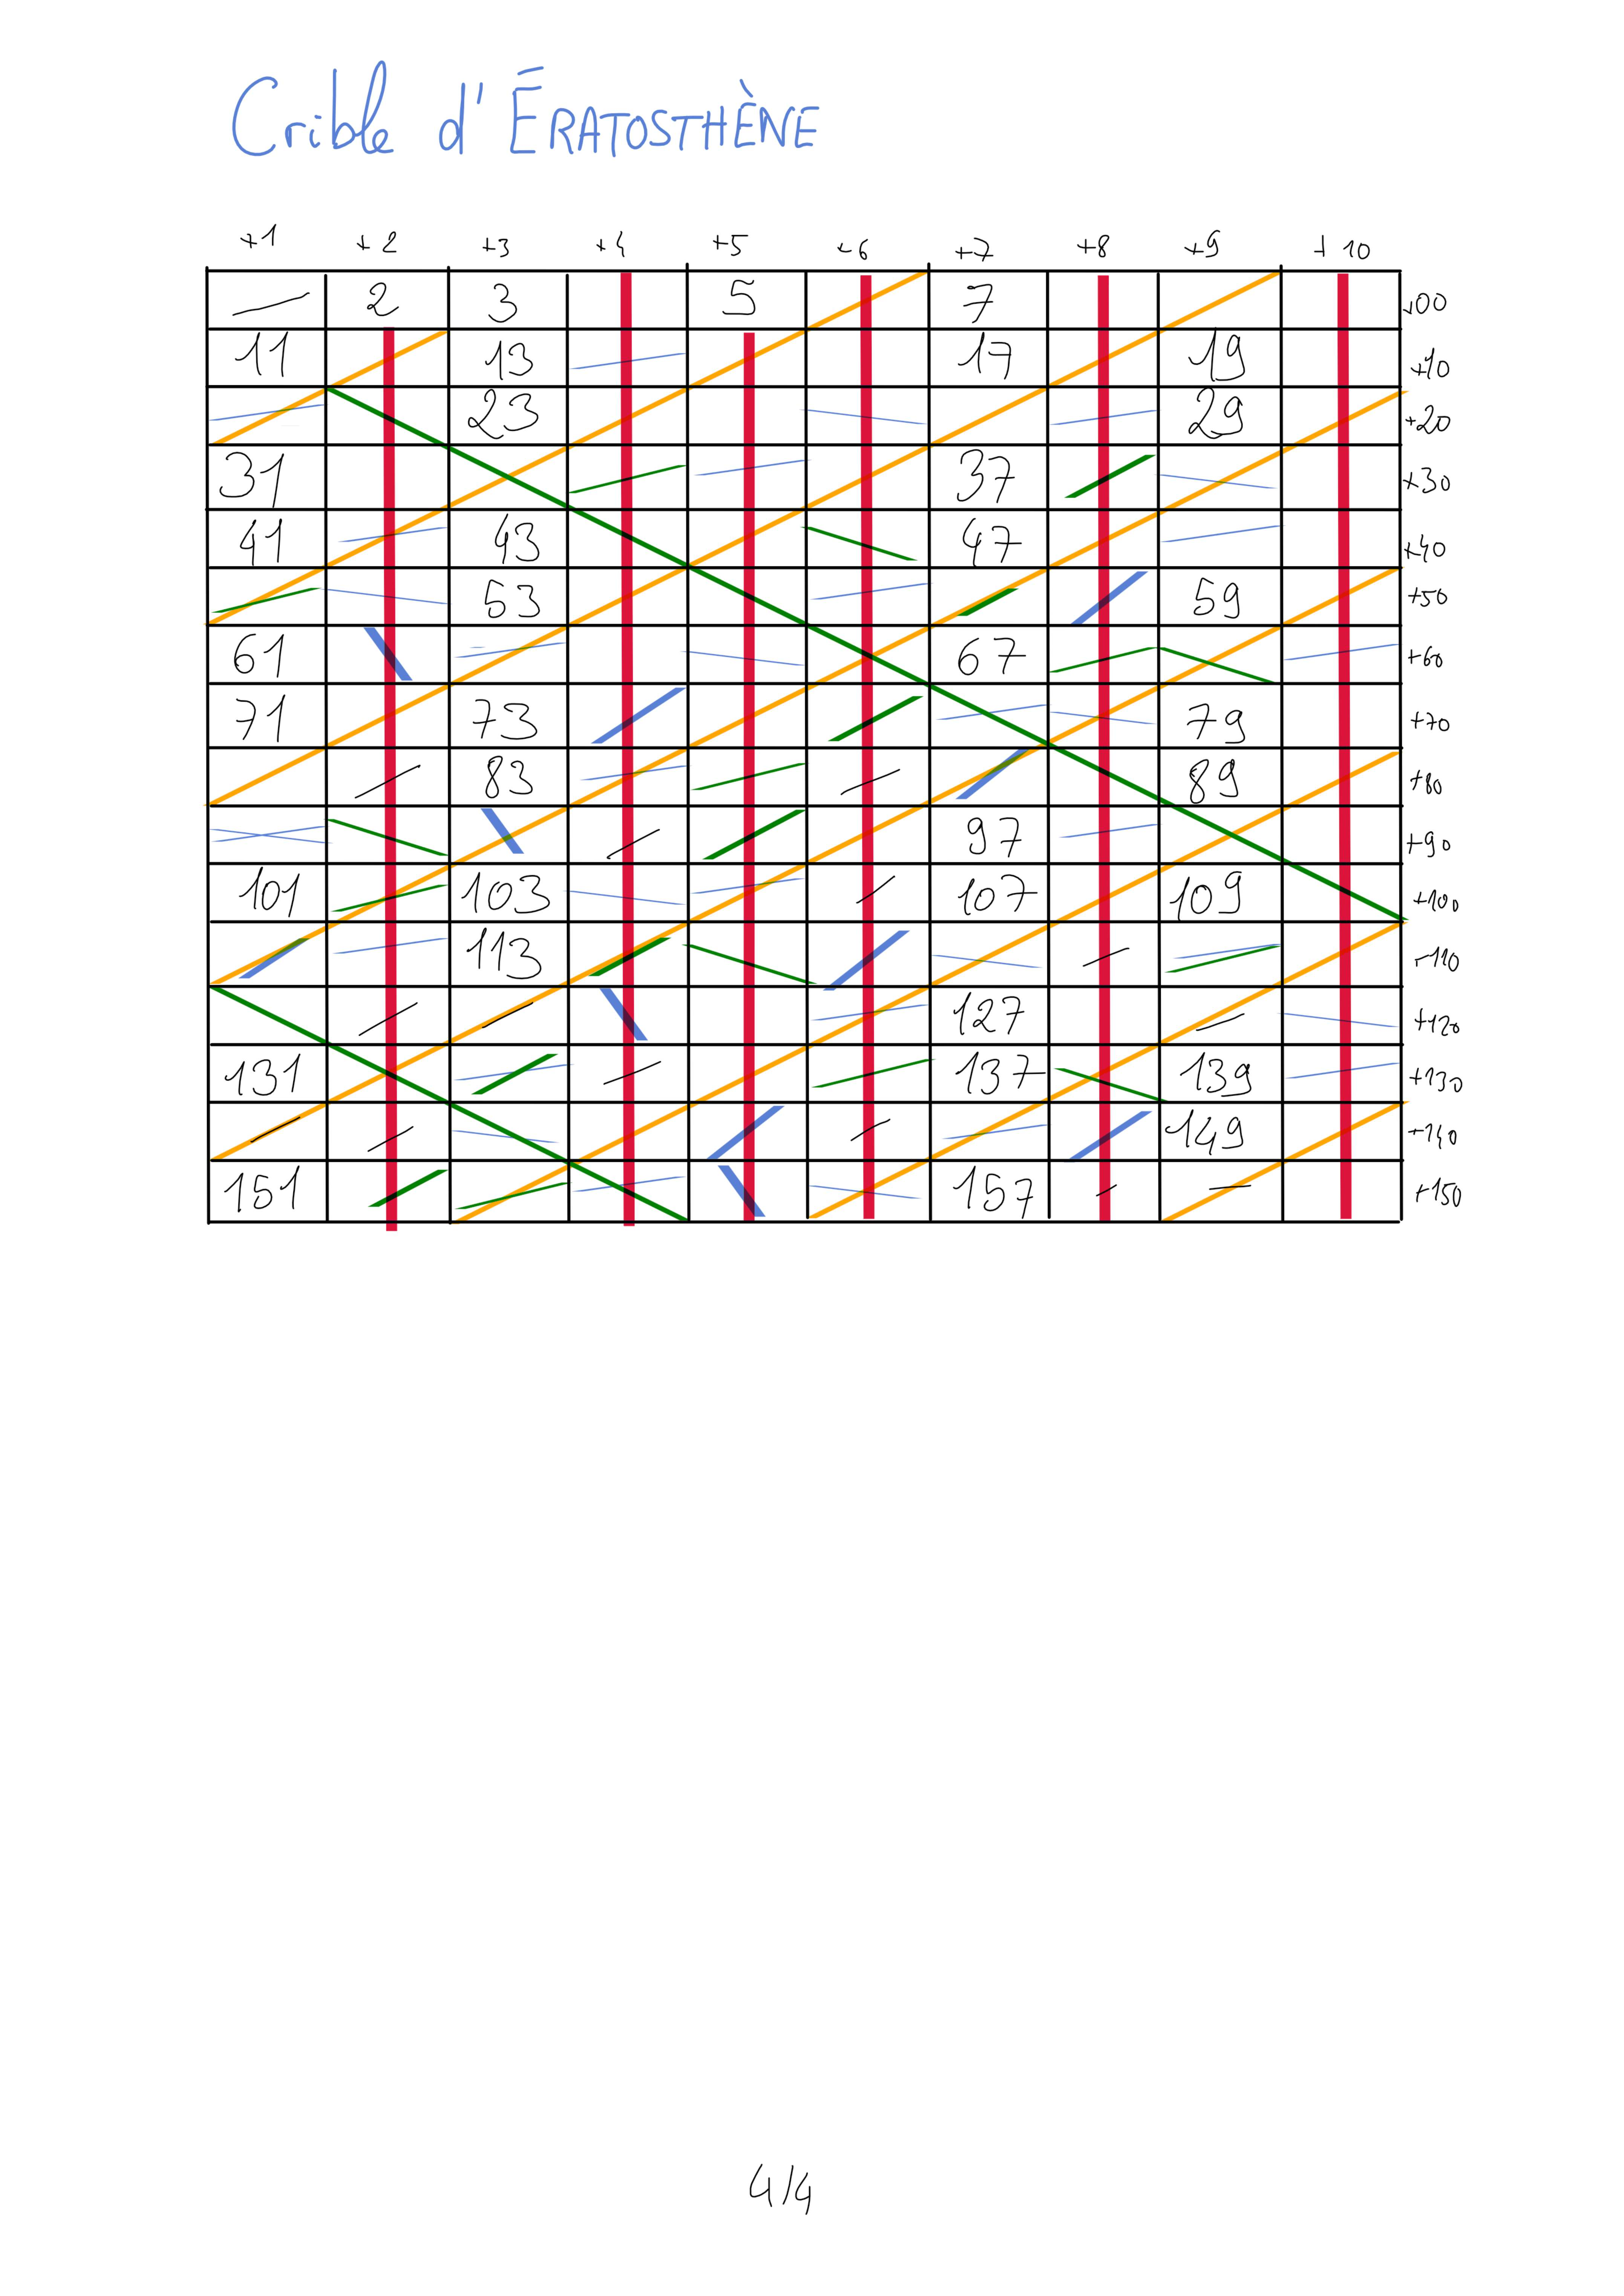
\includegraphics[trim={0 0 0 0},clip,width=1\linewidth]{img/eratosthene.pdf}
	\caption{Crible d'Eratosthène}
\end{figure}



\chapter*{123 : Corps finis. Applications.}
\setcounter{definition}{0}
\section*{I. Des corps finis}
\subsection*{A. Prérequis sur les extensions de corps}

\textcolor{paragraphtext}{Soit $L/M/K$ une tour d'extensions de corps (commutatifs).}

\begin{proposition_def}[\textnormal{[P] 65}]
	$L$ est un $K$-espace vectoriel, sa dimension est appelée \emph{degré de $L/K$}, et est notée $\left[L:K\right]$.
\end{proposition_def}

\begin{theorem}[de la base téléscopique - \textnormal{[P] 65}]
	Soient $\left(e_i\right)_{i\in I}$ une base $K$-base de $M$ et $\left(f_j\right)_{j\in K}$ une $M$-base de $L$,
	alors $\left(e_if_j\right)_{(i,j)\in I\times J}$ est une $K$-base de $L$.
	En particulier, $[L:K] = [L:M]\times [M:K]$ (dans $\IN\cup \left\{+\infty\right\})$.
\end{theorem}

\begin{definition}[\textnormal{[P] 70}]
	Soit $P\in K[X]$ non constant.
	Supposons $P$ irréductible sur $K$. On dit que $L$ est un \emph{corps de rupture} (CDR) de $P$ sur $K$ s'il existe $\alpha\in L$ tel que $P(\alpha) = 0$ et $L=K(\alpha)$.
	
	On dit que $L$ est un \emph{corps de décomposition} (CDD) de $P$ sur $K$ s'il existe $(\alpha_1,\dots,\alpha_n)\in L^n$ tel que $L = K(\alpha_1,\dots,\alpha_n)$ et $P$ est scindé sur $L$.
\end{definition}

\begin{theorem}[\textnormal{[P] 70-71}]
	$P$ admet un unique corps de rupture à $K$-isomorphisme près.
	Plus précisément, $K[X]/\langle P \rangle$ est un corps de rupture de $P$ sur $K$.

	$P$ admet un unique corps de décomposition $D$ à $K$-isomorphisme près. Celui-ci vérifie $[D:K]\leq \deg(P)!$.
\end{theorem}

\subsection*{B. Construction des corps finis : existence et unicité}

\textcolor{paragraphtext}{Dans ce paragraphe $K$ désigne un corps fini commutatif.}

\begin{example}
	Soit $p$ un nombre premier. L'anneau $(\IZpZ, +,\times )$ est un corps fini commutatif. On le note $\IF_p$.
\end{example}

\begin{theorem_def}[\textnormal{[P] 72}]
	Il existe un nombre premier $p$ rendant le diagramme suivant commutatif :
		$$\begin{tikzcd}
			{\mathbb{Z}} && K \\
			& {\mathbb{Z}/p\mathbb{Z}}
			\arrow["{n\mapsto n\cdot 1_K}", from=1-1, to=1-3]
			\arrow[two heads, from=1-1, to=2-2]
			\arrow[hook, from=2-2, to=1-3]
		\end{tikzcd}$$
	L'entier $p$ est appelé \emph{caractéristique} de $K$ notée $\car K$ et $\IF_p$ est appelé \emph{sous-corps premier de $K$}.
	C'est le plus petit sous-corps de $K$.
\end{theorem_def}

\textcolor{paragraphtext}{On notera $p$ la caractéristique de $K$.}

\begin{corollary}[\textnormal{[P] 72}]
	$\#K = p^{\left[K\,\colon \IF_p\right]}$
\end{corollary}
\begin{remark}
	Il n'existe pas de corps fini commutatif à $6$ éléments !
\end{remark}

\begin{lemma_def}[\textnormal{[P] 73}]
	$\textnormal{Fr}\,\colon K\to K$, $x\mapsto x^p$ est un morphisme de corps, appelé \emph{morphisme de Fröbenius}.
\end{lemma_def}

\begin{theorem}[\textnormal{[P] 73}]
	Soient $r\in \IN^*$, $p$ premier et $q=p^r$. Il existe un corps fini commutatif à $q$ éléments.
	Un tel corps est un CDD de $X^q - X$. En particulier, les classes d'isomorphisme de corps finis commutatifs sont caractérisées par le cardinal de ces derniers.
	On note $\IF_q$ un représentant de la classe d'isomorphisme des corps finis commutatifs à $q$ éléments.
\end{theorem}

\begin{theorem}[de Wedderburn - \textnormal{[P] 82}]
	Tout corps fini est commutatif.
\end{theorem}

\begin{example}
	$\IF_4 = \IF_2[X] / \langle X^2+X+1\rangle = \left\{0, 1, \overline{X}, 1 + \overline{X}\right\}$.

	$\IF_9 = \IF_3[X] / \langle X^3 + X^2 + X +1\rangle$.
\end{example}

\subsection*{C. Proprriétés des corps finis}

\textcolor{paragraphtext}{Soient $p$ un nombre premier, $r\in \IN^*$ et $q=p^r$.}

\begin{proposition}[\textcolor{myred}{FIG. 1}]
	$\forall (m,n)\in\left(\IN^*\right)^2$, $\IF_{p^n}\subseteq \IF^{p^m} \iff n\mid m$.
\end{proposition}

\begin{proposition}[\textnormal{[P] e73}]
	\begin{itemize}
		\item $\overline{\IF_p} = \bigcup_{n\in\IN^*}\IF_{p^n}$ est une clôture algébrique de $\IF_p$.
		\item Si $K$ est une extension de $\IF_q$, alors $\IF_q=\left\{x\in K \mid x^q = x\right\}$. En particulier, $\IF_q$ est l'unique sous-corps de $\overline{\IF_p}$ de cardinal $q$.
	\end{itemize}
\end{proposition}

\begin{theorem}[\textnormal{[P] 74}]
	$\IF_q^{\times}$ est cyclique.
\end{theorem}

\begin{proposition}[\textnormal{[P] 73}]
	$\textnormal{Fr}$ est un automorphisme de $\IF_q$.
\end{proposition}

\begin{theorem}[\textnormal{[R] 425}]
	Le groupe des automorphismes de $\IF_q$ est cyclique d'ordre $r$, engendré par $\textnormal{Fr}$.
\end{theorem}

\begin{remark}
	Pour tout $\theta\in\IF_q$, il existe $d\in\IN^*$ tel que $\textnormal{Fr}^d(\theta) = \theta^{dp} = \theta$.
	Le polynôme minimal de $\theta$ sur $\IF_p$ est $\prod_{k=1}^{d}\left(X-\textnormal{Fr}^k(\theta)\right)$.
\end{remark}

\begin{example}
	Soit $\beta = \overline{X}^2 + \overline{X} \in \IF_2[X]/\langle X^4 + X + 1\rangle$. On a $P_{\beta, \IF_2} = X^2 + X + 1$.
\end{example}

\section*{II. Carrés dans un corps fini}

\textcolor{paragraphtext}{
	Soient $p$ un nombre premier \emph{impair}, 
	$r\in\IN^*$ et $q = p^r$. 
	On pose $c\,\colon\IF_q\to\IF_q$, $x\mapsto x^2$ 
	et $l\,\colon \IF_q\to\IF_q$, $x\mapsto x^{\frac{q-1}{2}}$.}

\begin{proposition}
	$\im l = \Ker c = \left\{\pm 1\right\}$ et $\Ker l = \im c = \left\{x^2\mid x\in \IF_q^{\times}\right\}$.
\end{proposition}

\begin{corollary}[Critère d'Euler - \textnormal{[P] 75}]
	$x\in\IF_q^{\times}$ est un carré si, et seulement si $x^{\frac{q+1}{2}}=1$.
\end{corollary}

\begin{corollary}[\textnormal{[P] 74}]
	Il y a $\frac{q-1}{2}$ carrés inversibles dans $\IF_q$ (et $\frac{q+1}{2}$ carrés).
\end{corollary}

\begin{proposition}[\textnormal{[P] 74}]
	Tous les éléments de $\IF_{2^r}$ sont des carrés.
\end{proposition}

\begin{proposition}[\textnormal{[P] 75}]
	$-1$ est un carré dans $\IF_p$ si, et seulement si, $p\equiv 1\,[4]$.
\end{proposition}

\begin{application}[\textnormal{[P] 56}]
$p$ est la somme de deux carrés si, et seulement si, $p=2$ ou $p\equiv 1\,[4]$.
\end{application}

\begin{definition}[\textnormal{[R] 428}]
	Le \emph{symbole de Legendre de $a\in\IZ$ modulo $p$} est défini par :
	\begin{align*}
		\left(\frac{a}{b}\right) = \begin{cases}
			0\quad \text{si } a\in p\IZ \\
			1\quad \text{si $a$ est un carré inversible modulo $p$} \\
			-1\quad \text{sinon}
		\end{cases}
	\end{align*}
\end{definition}

\begin{proposition}[\textnormal{[R] 428}]
	$\forall a\in\IZ$, $\left(\frac{a}{p}\right)\equiv a^{\frac{p-1}{2}}$.
	En particulier, $\left(\frac{\cdot}{p}\right)$ est un morphisme du groupe $\IF_p^{\times}$.
\end{proposition}



\begin{tcolorbox}[
    breakable, % Allows the theorem to split across pages
    colback=developpement, % The background color
    colframe=gray!0!black, % The frame color
    boxrule=0pt, % The frame thickness
    arc=1mm, % Sharp corners
	boxsep=0pt,
	left=0pt, right=0pt, top=0pt, bottom=0pt
]
\begin{proposition}[\textnormal{[R] 431-434}]
	\label{123dev11}
	Soit $a\in\IF_p^{\times}$. L'équation de $ax^2 = 1$ a $1+\left(\frac{a}{p}\right)$ solutions dans $\IF^p$.
\end{proposition}
\begin{theorem}[Loi de réciprocité quadratique - \textnormal{[R] 431-434}]
	\label{123dev12}
	Soient $p$ et $q$ deux nombres premiers impairs distincts.

	\begin{align*}
		\left(\frac{p}{q}\right)\left(\frac{q}{p}\right) = \left(-1\right)^{\frac{p-1}{2}\frac{q-1}{2}}
	\end{align*}
\end{theorem}
\end{tcolorbox}

\begin{application}
	$\left(\frac{11}{23}\right) = \left(\frac{23}{11}\right)\left(-1\right)^{11\cdot 5} = -\left(\frac{1}{11}\right) = -1$ donc $11$ n'est pas un carré modulo $23$.
\end{application}

\begin{proposition}[\textnormal{[R] e438, [C] 307}]
	$\left(\frac{2}{p}\right) = \left(-1\right)^{\frac{p^2 - 1}{8}}$
\end{proposition}

\begin{proposition}
	Soit $(a,b,c)\in\IF_q^3$ avec $a \neq 0$. L'équation $ax^2 + bx + C = 0$ dans $\IF_q$ 
	possède des solutions si, et seulement si, $b^2-4ac$ est un carré dans $\IF_q$. Le cas échéant, si $\delta\in/IF_p$ vérifie $\delta^2 = b^2-4ac$, alors 
	les solutions de cette équation sont $\frac{-b\pm \delta}{2a}$.
\end{proposition}

\begin{remark}
	Dans $\IF_{2r}$, l'équation $ax^2+bx+c=0$ est bien plus difficile à résoudre, en dehors des cas triviaux !
\end{remark}

\section*{III. Algèbre (bi)linéaire sur les corps finis}

\textcolor{paragraphtext}{Soient $p$ un nombre premier impair, $r\in\IN^*$, $q = p^r$ et $n\in\IN$.}

\begin{proposition}[\textnormal{[R] 155}]
	\begin{itemize}
		\item $\# GL_n(\IF_q) = (q^n-1)(q_n - q)\dots (q^n-q^{n-1}) = q^{\frac{n(n-1)}{2}}\prod_{k=1}^{n}(q^k-1)$
		\item $\# SL_n(\IF_q) = \#GL_n(\IF_q)/(q-1)$
	\end{itemize}
\end{proposition}

\begin{tcolorbox}[
    breakable, % Allows the theorem to split across pages
    colback=developpement, % The background color
    colframe=gray!0!black, % The frame color
    boxrule=0pt, % The frame thickness
    arc=1mm, % Sharp corners
	boxsep=0pt,
	left=0pt, right=0pt, top=0pt, bottom=0pt
]
\begin{theorem}[\textnormal{[C] 50}]
	\label{123dev2}
	\begin{align*}
		SO_2(\IF_q)\cong \begin{cases}
			\IZ/(q-1)\IZ\quad\text{si $-1$ est un carré mod $q$} \\
			\IZ/(q+1)\IZ\quad\text{sinon}
		\end{cases}
	\end{align*}
\end{theorem}
\end{tcolorbox}

\begin{remark}
	$SO_2(\IF_{2^r}) = \begin{pmatrix}
		0 & 1 \\
		1 & 0
	\end{pmatrix} + \IF_{2^r}\begin{pmatrix}
		1 & 1 \\ 1 & 1
	\end{pmatrix}$, puis $SO_2(\IF_{2^r})\cong \left(\IZ/2\IZ\right)^r$.
\end{remark}

\textcolor{paragraphtext}{Soit $E$ un $\IF_q$-espace vectoriel de dimension finie.}

\begin{definition}[\textnormal{[R] 463}]
	Le \emph{discriminant} d'une forme quadratique $f$ sur $E$ est l'image de son déterminant dans une base quelconque modulo les carrés de $\IF_q^{\times}$.
\end{definition}

\begin{theorem}[\textnormal{[R] e482}]
	Il y a deux classes d'équivalence de formes quadratiques non-dégénérées sur $E$.
	Plus précisément, soient $\alpha\in\IF_q^{\times}$ qui n'est pas un carré, et $f$ une forme 
	quadratique sur, de matrice $M$ dans la base canonique.

	\begin{itemize}
		\item Si $\det M$ est un carré dans $\IF_p^{\times}$, alors $M$ est congruente à la matrice $\diag(1,1,\dots, 1,1)$.
		\item Sinon, $M$ est congruente à $\diag(1,1,\dots, 1, \alpha)$.
	\end{itemize}
\end{theorem}

\begin{application}
	Loi de réciprocité quadratique (Thm \ref{123dev12}).
\end{application}

\section*{IV. Polynômes et corps finis}

\begin{theorem}[Critère d'Eisenstein - \textnormal{[P] 76}]
	Soit $P = \sum_{k=0}^{n} a_kX^k\in\IZ[X]$.
	Soit $p$ un nombre premier. Si $p\nmid a_n$, si $\forall k\in \llbracket 0, n-1\rrbracket$, $p\mid a_k$ et $p^2\nmid a_0$, alors $P$ est irréductible dans $\IQ[X]$.
\end{theorem}

\begin{example}
	Pour tout $p$ premier, $\Phi_p = X^{p+1} + \dots + X + 1$ est irréductible sur $\IQ$.
\end{example}

\begin{theorem}[\textnormal{[P] 77}]
	Soit $P = \sum_{k=0}^{n} a_kX^k\in\IZ[X]$, $n\geq 1$, $a_n\neq 0$.
	Soit $p\in\IZ$ premier. Si $p\nmid a_n$ et si l'image $\overline{P}$ de $P$ 
	dans $\IF_p[X]$ est irréductible, alors $P$ est irréductible sur $\IZ$.
\end{theorem}

\begin{remark}
	La réciproque est fausse : considérer $X^4 + 1$.
\end{remark}

\section*{Développements}
\begin{itemize}
	\item Développement 1 : Proposition \ref{123dev11}, et théorème \ref{123dev12} : loi de réciprocité quadratique (par les formes quadratiques)
	\item Développement 2 : Théorème \ref{123dev2}
\end{itemize}

\section*{Références}
\begin{itemize}
	\item[R] \emph{Mathématiques pour l'agrégation - Algèbre et géométrie}, Jean-Étienne Rombaldi, 2e édition
	\item[P] \emph{Cours d'algèbre}, Perrin
	\item[C] \emph{Nouvelles histoires hédonistes de groupes et géométries}, P. Caldero, J. Germoni
\end{itemize}

\begin{figure}[!htb]
	\centering
	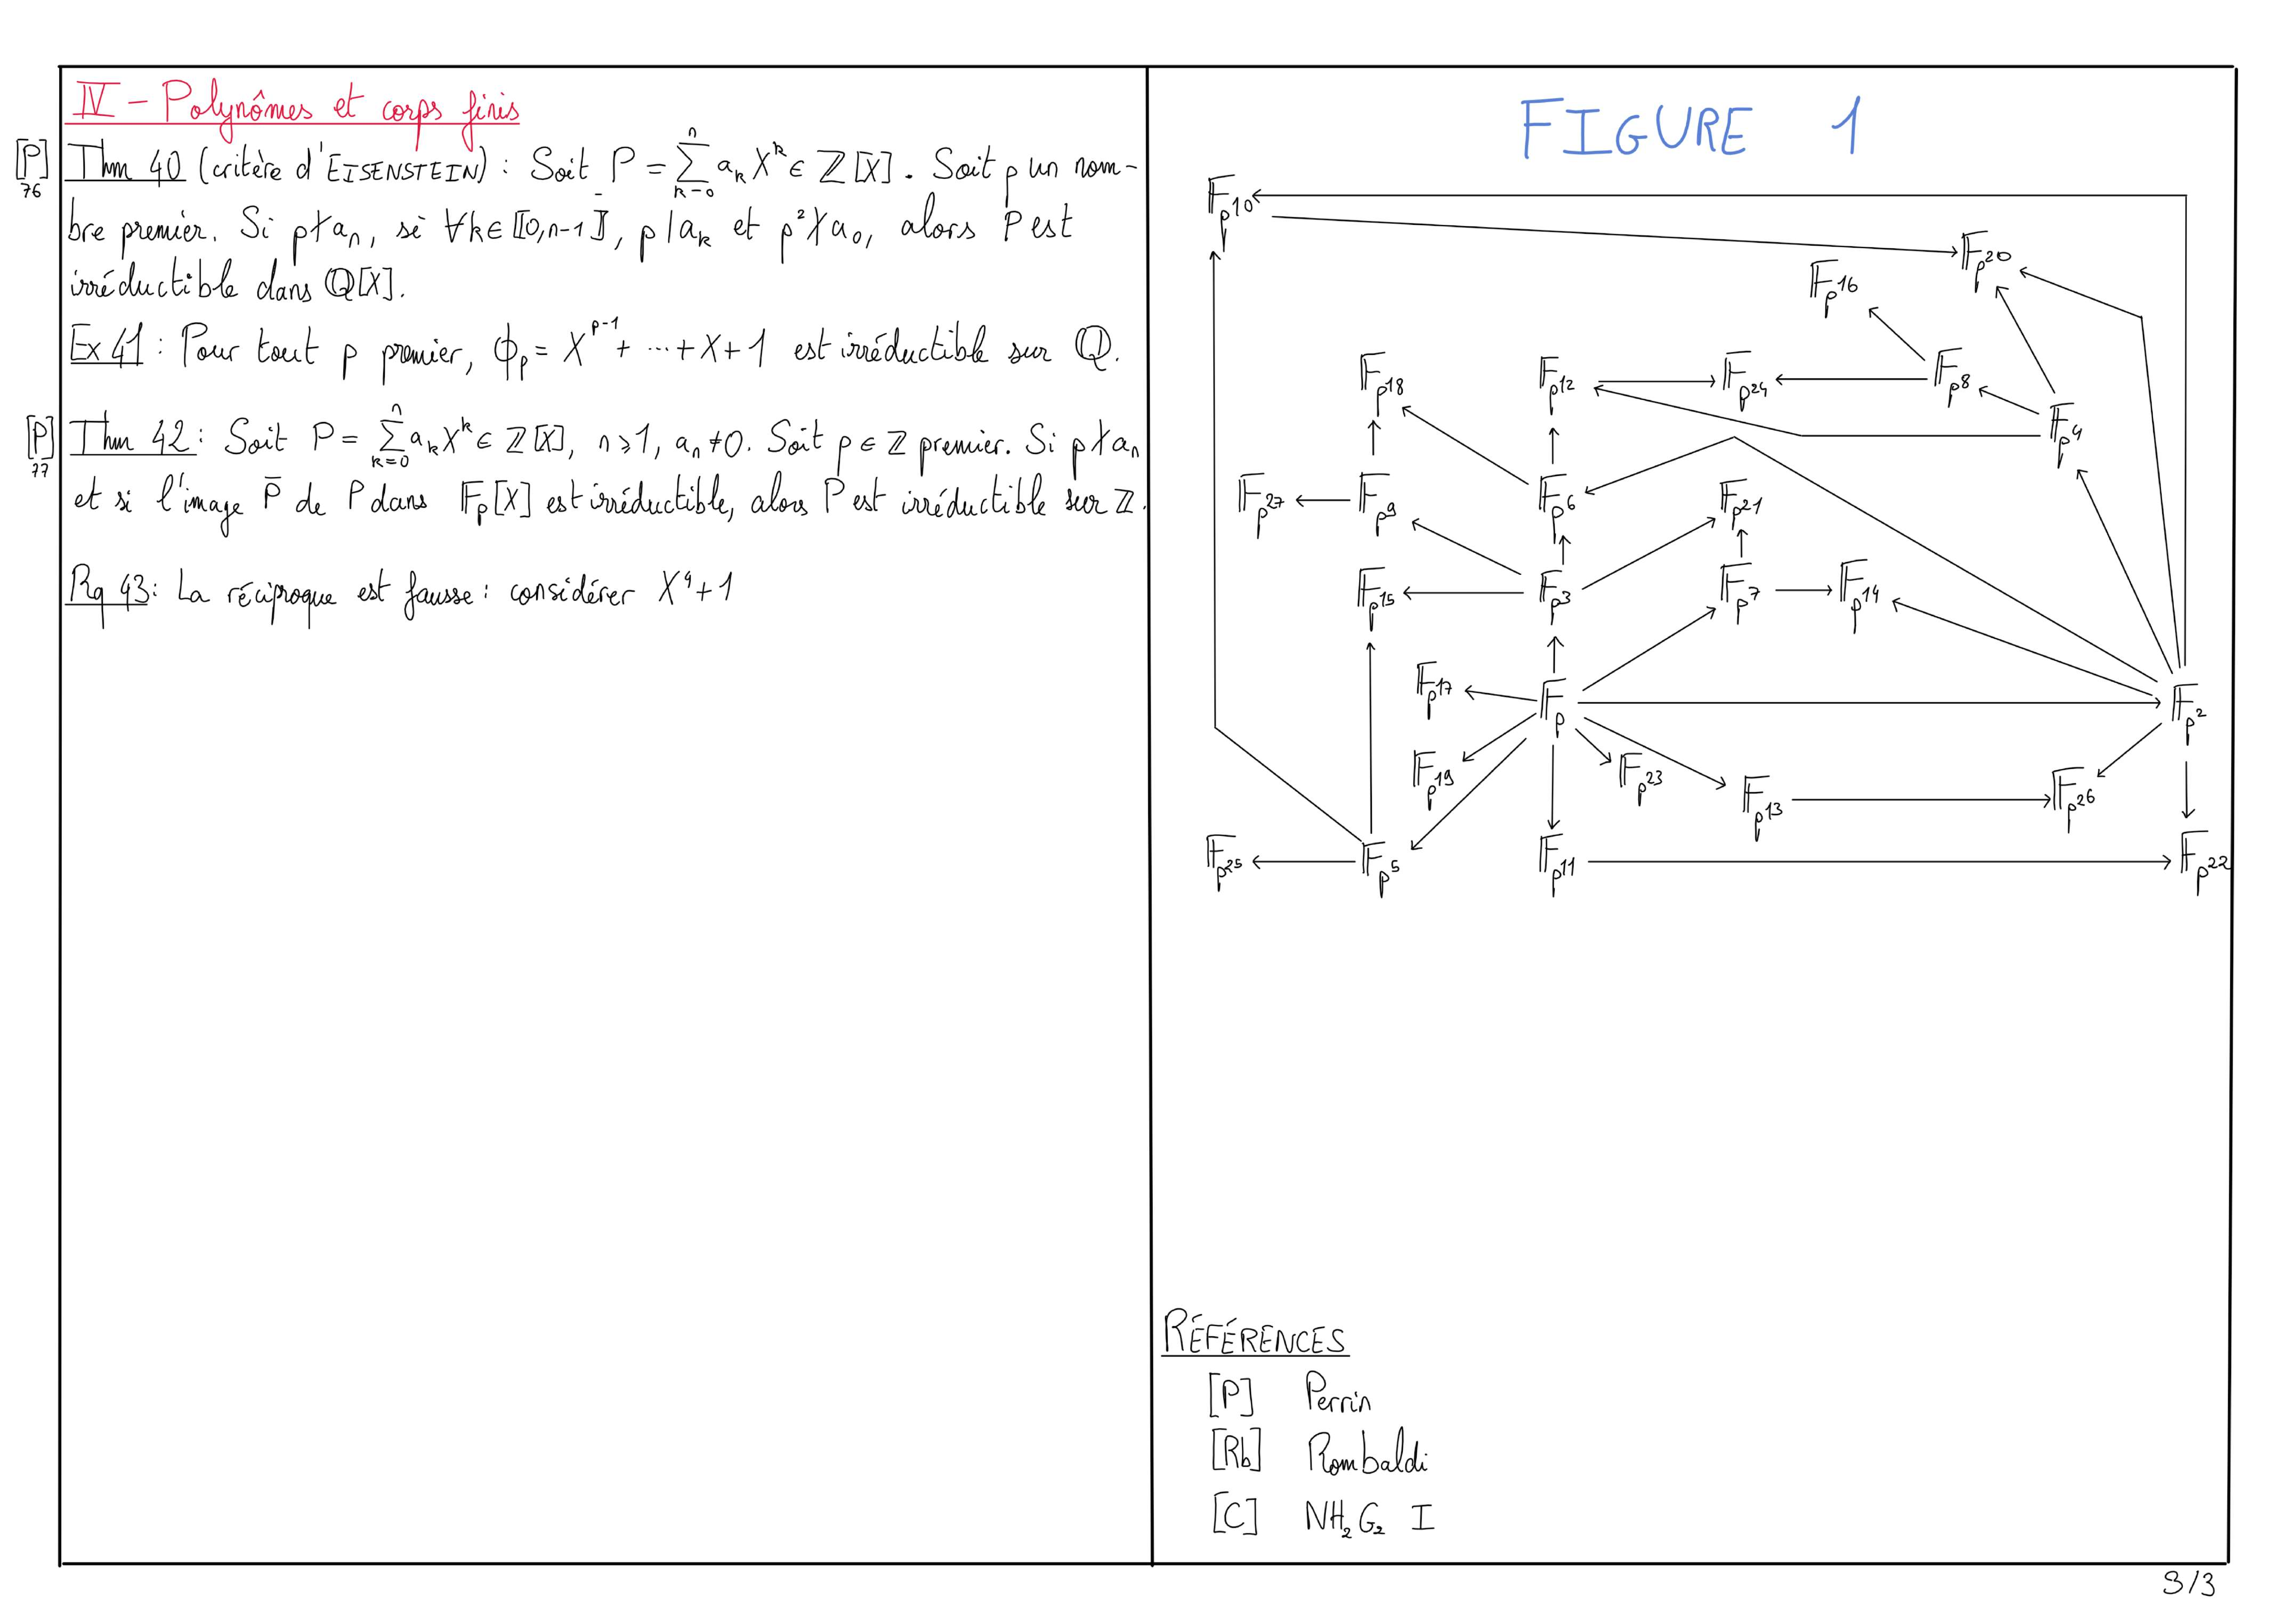
\includegraphics[trim={0 0 0 0},clip,width=1\linewidth]{img/diagramme_extensions_corps_finis.pdf}
	\caption{Diagramme des extensions de corps finis}
\end{figure}


\chapter*{141 : Polynômes irréductibles à une indéterminée. Corps de rupture. Exemples et applications.}
\setcounter{definition}{0}
\textcolor{paragraphtext}{Soient $A$ un anneau unitaire intègre commutatif, et $L/K$ une extension de corps commutatif. Soit $P\in A[X]$.}

\section*{I. Polynômes irréductibles}
\subsection*{A. Notion d'irréductibilité pour les polynômes}

\begin{definition}[\textnormal{[R] 370}]
		On dit que $P$ est \emph{irréductible sur $A$} si $P\notin A[X]^{\times} = A^{\times}$, si $P\neq 0$ et si :
		$\forall(P_1,P_2)\in A[X]^2$, $P = P_1P_2 \implies P_1\in A^{\times}$ ou $P_2\in A^{\times}$.
\end{definition}

\begin{example}[\textnormal{[R] 370}]
	Tout polynôme de degré $1$ est irréductible ; et les polynômes réels de degré $2$ de discriminant $< 0$ sont irréductibles.
\end{example}

\begin{proposition}[\textnormal{[R] 371}]
	\begin{itemize}
		\item Si $P\in K[X]$ est irréductible et si $\deg P > 1$ , alors $P$ n'a pas de racine dans $K$.
		\item Si $P\in K[X]$ n'a pas de racine dans $K$ et si $\deg P \leq 3$, alors $P$ est irréductible sur $K$.
	\end{itemize}
\end{proposition}

\begin{example}
	\begin{itemize}
		\item $(x^2+1)^2$ est réductible sur $\IR$ et sans racine dans $\IR$.
		\item Les polynômes irréductibles de petit degré de $\IF_2[X]$ sont $X$, $X+1$, $X^2+X+1$.
	\end{itemize}
\end{example}

\subsection*{B. Proprétés de $A[X]$}
\begin{proposition}[\textnormal{[R] 374}]
	$A[X]$ euclidien $\iff A[X]$ principal $\iff A$ est un corps.
\end{proposition}

\begin{proposition}[\textnormal{[R] e375}]
	Si $P\in K[X]$ est irréductible, alors $K[X]/\langle P\rangle$ est un corps.
\end{proposition}

\textcolor{paragraphtext}{On suppose $A$ factoriel.}

\begin{definition}[\textnormal{[S] 547-548; [P] 51}]
	Le \emph{contenu de $P\in A[X]\setminus \left\{0\right\}$}, noté $c(P)$, est un PGCD des coefficients de $P$.
	On dit que $P$ est \emph{primitif} si $c(P)\in A^{\times}$.
\end{definition}

\begin{theorem}[\textnormal{[P] 51; [S] 548}]
	Soit $P\in A[X]$ primitif non constant. $P$ est irréductible dans $A[X] \iff A$ est irréductible dans $K[X]$.
\end{theorem}

\begin{example}
	Soient $a_1,\dots,a_n$ des entiers distincts. Le polynôme $(X-a_1)\dots (X-a_n) - 1$ est irréductible sur $\IQ$.
\end{example}

\begin{lemma}
	Un produit de polynômes primitifs est primitif.
\end{lemma}

\begin{tcolorbox}[
    breakable, % Allows the theorem to split across pages
    colback=developpement, % The background color
    colframe=gray!0!black, % The frame color
    boxrule=0pt, % The frame thickness
    arc=1mm, % Sharp corners
	boxsep=0pt,
	left=0pt, right=0pt, top=0pt, bottom=0pt
]
\begin{lemma}[de Gauss - \textnormal{[S] 548; [P] 51}]
\label{141dev1a}
	$c(PQ) = c(P)c(Q)$
\end{lemma}
\end{tcolorbox}

\begin{theorem}[\textnormal{[R] 358; [S] 548; [P] 51}]
	$A[X]$ est factoriel $\iff A$ est factoriel.
\end{theorem}

\subsection*{C. Critères d'irréductibilité}

\begin{theorem}[Critère d'Eisenstein - \textnormal{[S] 549; [P] 76}]
	Ecrivons $P=\sum_{k=0}^{n} a_kX^k$, $a_n \neq 0$.
	S'il existe $p\in A$ premier non nul tel que $\forall k\in \llbracket 1,n-1\rrbracket$, $p\mid a_k$, $p^2 \nmid a_0$ et $p\nmid a_n$, alors $P$ est irrductible dans $\Frac(A)[X]$.
\end{theorem}

\begin{example}
	$\forall n\geq 2$, $\forall d\in\IN^*$ sans facteur carré, $X^n - d$ est irréductible dans $\IZ[X]$.
\end{example}

\begin{theorem}[\textnormal{[P] 77}]
	Soit $I$ un idéal de $A$. Ecrivons $P = \sum_{k=0}^{n} a_kX_k$, $a_n\neq 0$.
	Si $a_n \not\equiv 0$ mod $I$ et si $P$ mod $I$ est irréductible dans $\left(A/I\right)[X]$ alors
	$P$ est irréductible dans $A[X]$.
\end{theorem}

\begin{example}[\textnormal{[P] 77}]
	Pour tout $p$ premier, $X^p-X-1$ est irréductible sur $\IQ$.
\end{example}

\section*{II. Polynômes et extensions de corps}
\textcolor{paragraphtext}{Soient $L$ et $K$ deux corps commutatifs. Soit $P\in K[X]$.}

\subsection*{A. Extensions de corps, éléments algébriques}
\begin{definition}[\textnormal{[P] 65}]
	On dit que $L$ est \emph{une extension de $K$}, et on note $L/K$, si $K\subseteq L$.
\end{definition}

\begin{proposition_def}[\textnormal{[P] 65}]
	$L$ est un $K$-espace vectoriel dont on note $[L:K]$ la dimension, que l'on appelle \emph{degré de l'extension $L/K$}.
	On dit que $L/K$ est finie si $[L:K]$ est fini.
\end{proposition_def}

\begin{theorem}[de la base téléscopique - \textnormal{[P] 65}]
	Soient $\left(e_i\right)_{i\in I}$ une base $K$-base de $M$ et $\left(f_j\right)_{j\in K}$ une $M$-base de $L$,
	alors $\left(e_if_j\right)_{(i,j)\in I\times J}$ est une $K$-base de $L$.
\end{theorem}

\begin{corollary}[Multiplicativité des degrés - \textnormal{[P] 65}]
	$[L:K] = [L:M]\times [M:K]$
\end{corollary}

\begin{definition}[\textnormal{[P] 66}]
	On dit que $\alpha\in L$ est \emph{algébrique sur $K$} s'il existe $P\in K[X]$ tel que $P(\alpha)=0$.
	Sinon, on dit que $\alpha$ est \emph{transcendant}.
\end{definition}

\begin{theorem_def}[\textnormal{[P] 66}]
	Si $\alpha\in L$ est algébrique sur $K$, alors $\left\{P\in K[X]\mid P(\alpha) = 0\right\}$
	est un idéal non nul, qui donc admet un unique générateur unitaire $P_{\alpha, K}$ appelé \emph{polynôme minimal de $\alpha$ sur $K$}.
\end{theorem_def}

\begin{notation*}
	$K[\alpha] = \left\{P(\alpha)\mid P\in K[X]\right\}$
\end{notation*}

\begin{theorem}[\textnormal{[P] 66}]
	Soit $\alpha\in L$. Sont équivalentes :
	\begin{enumerate}
		\item $\alpha$ est algébrique sur $K$
		\item $K[\alpha] = K(\alpha)$
		\item $K[\alpha]$ est un $K$-espace vectoriel de dimension finie.
	\end{enumerate}

	Le cas échéant, $\deg P_{\alpha, L} = [K(\alpha) : K]$.
\end{theorem}

\subsection*{B. Corps de rupture et de décomposition}

\begin{definition}[\textnormal{[P] 70}]
	Supposons $P$ irréductible. On dit que $L$ est un \emph{corps de rupture de $P$ sur $K$} s'il existe $\alpha\in L$ tel que $P(\alpha) = 0$ et $L=K(\alpha)$.
\end{definition}

\begin{theorem}[\textnormal{[P] 70}]
	Supposons $P$ irréductible. Le corps $K[X]/\langle P\rangle$ est un corps de rupture de $P$ sur $K$, et c'est le seul à isomorphisme près.
\end{theorem}

\begin{example}
	$\IC$ peut être défini comme $\IR[X]/\langle X^2 + 1 \rangle$.
\end{example}

\begin{application}
	Si $P$ est irréductible et si $\deg P \wedge [L:K]$, alors $P$ est irréductible sur $L$.
\end{application}

\begin{definition}[\textnormal{[P] 71}]
	On dit que $L$ est un \emph{corps de décomposition de $P$ sur $K$} si $P$ est sciendé sur $L$ et si $L = K(\alpha_1,\dots,\alpha_n)$ avec $\alpha_1,\dots,\alpha_n$ les racines de $P$.
\end{definition}

\begin{theorem}[\textnormal{[P] 71}]
	Il existe un corps de décomposition de $P$ sur $K$, unique à isomorphisme près.
\end{theorem}

\begin{example}[\textnormal{[P] 72}]
	$\IQ(j,\sqrt[3]{}2)$ est un corps de décomposition de $X^3 - 2$ sur $\IQ$.
\end{example}

\begin{theorem}[de l'élément primitif - \textnormal{[P] 87}]
	Toute extension finie d'un corps de caractéristique nulle est monogène.
\end{theorem}

\subsection*{C. Clôture algébrique}
\begin{definition}[\textnormal{[P] 67}]
	On dit que $K$ est \emph{algébriquement clos} si tout polynôme non nul de $K[X]$ est scindé, et si $K$ n'admet pas d'extension algébrique non triviale.
\end{definition}

\begin{definition}[\textnormal{[P] 72}]
	On dit que $L$ est une \emph{clôture algébrique} de $K$ si c'est une extension de $K$ algébrique et algébriquement close.
\end{definition}

\begin{example}[\textnormal{[P] 68-72}]
	\begin{itemize}
		\item $\IC$ est algébriquement clos (théorème de d'Alembert-Gauss) ;
		\item $\IC$ est une clôture algébrique de $\IR$.
	\end{itemize}
\end{example}

\begin{example}[\textnormal{[G] 94}]
	Si $L$ est algébriquement clos, alors l'ensemble des éléments de $L$ algébriques sur $K$ est un corps algébriquement clos.
\end{example}

\begin{theorem}
	$K$ admet une unique clôture algébrique à isomorphisme près.
\end{theorem}

\section*{III. Polynôme cyclotomiques}
\textcolor{paragraphtext}{On note $\IU := \left\{z\in \IC\mid z^n = 1\right\}$ le groupe des racines complexes $n$-ièmes de l'unité,
et $\mu_n^*$ l'ensemble de ses générateurs (que l'on appelle \emph{racines primitives $n$-ièmes de l'unité}).}

\begin{definition}[\textnormal{[P] 80; [R] 385}]
	Pour $n\in\IN^*$, on définit le \emph{$n$-ième polynôme cyclotomique} :
	$$\Phi_n = \prod_{\zeta\in \mu_n^*} X-\zeta$$
\end{definition}

\begin{proposition}[\textnormal{[P] 80-83; [R] 386}]
	On a les propriétés suivantes :
	\begin{itemize}
		\item Pour $\zeta_n\in\mu_n^*$, $$\Phi_n = \prod_{\substack{k=1 \\ k\wedge n = 1}}^{n} X - \zeta_n^k$$
		\item $X^n - 1 = \prod_{d\mid n} \Phi_d$
		\item $\Phi_n\in\IZ[X]$
	\end{itemize}
\end{proposition}

\begin{example}[\textnormal{[P] 81}]
		\begin{itemize}
			\item Pour $p$ premier, $\Phi_p = X^{p-1}+\dots X + 1$
			\item $\Phi_1 = X - 1$, $\Phi_4 = X^2 + 1$, $\Phi_6 =X^2 - X + 1$, $\Phi_8 = X^4 + 1$
		\end{itemize}
\end{example}


\begin{tcolorbox}[
    breakable, % Allows the theorem to split across pages
    colback=developpement, % The background color
    colframe=gray!0!black, % The frame color
    boxrule=0pt, % The frame thickness
    arc=1mm, % Sharp corners
	boxsep=0pt,
	left=0pt, right=0pt, top=0pt, bottom=0pt
]
\begin{theorem}[\textnormal{[P] 82-83; [R] 392}]
	\label{141dev1b1}
	Soit $\zeta_n\in\mu_n^*$. Le polynôme minimal de $\zeta_n$ sur $\IQ$ est $\Phi_n$.
\end{theorem}

\begin{corollary}
	\label{141dev1b2}
	$\Phi_n$ est irréductible sur $\IQ$ et $[\IQ(\zeta) : \IQ] = \varphi(n)$.
\end{corollary}
\end{tcolorbox}

\section*{IV. Polynômes irréductibles des corps finis}

\begin{definition}[\textnormal{[R] 331}]
	La \emph{fonction de Moëbius} est définie par :
	\begin{align*}
		\mu\,\colon n\in\IN^* \mapsto \begin{cases}
			1\quad \text{si } n =1 \\
			(-1)^r\quad \text{si n est le produit de $r$ facteurs premiers distincts} \\
			0\quad\text{sinon}
		\end{cases}
	\end{align*}
\end{definition}


\begin{tcolorbox}[
    breakable, % Allows the theorem to split across pages
    colback=developpement, % The background color
    colframe=gray!0!black, % The frame color
    boxrule=0pt, % The frame thickness
    arc=1mm, % Sharp corners
	boxsep=0pt,
	left=0pt, right=0pt, top=0pt, bottom=0pt
]
\begin{theorem}[Formule d'inversion de Moëbius = \textnormal{[R] 333}]
	\label{141dev21}
	Soient $\left(u_n\right)_{n\in\IN^*}\in\IR^{\IN^*}$ et $\left(v_n\right)_{n\in\IN^*}\in\IR^{\IN^*}$.
	Si $\forall n\in\IN^*$, $u_n = \sum_{d\mid n} v_d$, alors $\forall n\in\IN^*$, $v_n = \sum_{d\mid n}\mu(\frac{n}{d})u_d$.
\end{theorem}
\begin{theorem}[\textnormal{[R] 423}]
	\label{141dev22}
	$P_n := X^{p^n}-X =\prod_{d\mid n}\prod_{\mathcal{U}_d(p)} P$ où $\mathcal{U}_d(p)$ est l'ensemble des 
	polynômes irréductibles unitaires de degré $d$ de $\IF_p[X]$.
\end{theorem}
\begin{corollary}[\textnormal{[R] 424}]
	\label{141dev23}
	$\#\mathcal{U}_n(p) = \frac{1}{n}\sum_{d\mid n}\mu(\frac{n}{d})p^d$
\end{corollary}
\end{tcolorbox}

\section*{Développements}
\begin{itemize}
	\item Développement 1 : Lemme de Gauss \ref{141dev1a}
	\item Développement 2 : Théorème \ref{141dev1b1} et Corollaire \ref{141dev1b2}
	\item Développement 2 : Théorème \ref{141dev21}, Théorème \ref{141dev22} et Corollaire \ref{141dev23}
\end{itemize}

\section*{Références}
\begin{itemize}
	\item[R] \emph{Mathématiques pour l'agrégation - Algèbre et géométrie}, Jean-Étienne Rombaldi, 2e édition
	\item[P] \emph{Cours d'algèbre}, Perrin
	\item[G] \emph{Les maths en tête - Algèbre et probabilités}, Xavier Gourdon, 3e édition
	\item[S] \emph{Algèbre pour la licence 3}, Szpirglas
\end{itemize}

\chapter*{142 : PGCD et PPCM, algorithmes de calcul. Applications.}
\setcounter{definition}{0}
\section*{I. Notion de PGCD et de PPCM dans différents types d'anneaux}
\textcolor{paragraphtext}{Dans cette section, $A$ est un anneau intègre (commutatif) et $(a,b,a_1,\dots,a_r)\in A^{r+2}$.}

\subsection*{A. Première définition, existence, cas des anneaux factoriels}

\begin{definition}
	Si $a_1,\dots,a_r \neq 0$, alors sous réserve d'existence, on appelle \emph{PGCD} (resp. \emph{PPCM})
	de $a_1,\dots, a_r$, noté $a_1\wedge \dots\wedge a_R$ ou $\pgcd(a_1,\dots,a_r)$ (resp. $a_1\vee\dots\vee a_r$ ou $\ppcm(a_1,\dots,a_r)$)
	un plus grand minorant (resp. un plus grand majorant) de $\left\{a_1,\dots, a_r\right\}$ pour la relation (binaire) de divisibilité.
	On pose par ailleurs $0\wedge 0 = 0\vee a = 0$.

	En particulier, le PGCD et le PPCM sont associatifs et commutatifs: $a\wedge b = b\wedge a$ et $a_1\wedge a_2 \wedge a_3\wedge a_4\wedge a_5 = (a_1\wedge a_2)\wedge(a_3\wedge a_4)\wedge a_6$.
\end{definition}

\begin{remark}
	Les PGCD (resp. PPCM) de $a_1,\dots, a_r$ sont tous associés. L'écriture $d = a_1\wedge\dots\wedge a_r$ est un abus signifiant que $d$ est \underline{un} PGCD de $a_1,\dots,a_r$.
\end{remark}

\begin{proposition}[\textnormal{[R] 246}]
	Si $a$ et $b$ ont un PPCM alors ils ont un PGCD $a\wedge b = ab(a\vee b)^{-1}$.
\end{proposition}

\begin{example}
	$3$ et $2+i\sqrt{5}$ ont un PGCD mais pas de PPCM dans $\IZ[i\sqrt{5}]$.
	$4$ et $2+2i\sqrt{3}$ n'ont pas de PGCD dans $\IZ[i\sqrt{3}]$.
\end{example}

\begin{definition}
	On dit que $a_1,\dots, a_r$ sont \emph{premiers entre eux} (dans leur ensemble)
	si $a_1\wedge \dots\wedge a_r = 1$. On dit que $a_1, \dots, a_r$ sont \emph{deux à deux premiers entre eux} 
	si $\forall(i,j)\in \llbracket 1,n\rrbracket^2$, $i\neq j\implies a_i\wedge a_j = 1$.
\end{definition}

\begin{theorem}[de Gauss - \textnormal{[R] 247}]
	$\forall (a,b,c)\in A^3$, $a\mid bc$ et $a\wedge b=1 \implies a\mid c$. 
\end{theorem}

\begin{proposition}[\textnormal{[R] 246}]
	Si toute paire d'éléments de $A$ admet un PGCD (on dit alors que $A$ est un anneau à PGCD),
	alors toute paire d'éléments de $A$ admet un PPCM, et la réciproque est vraie.
\end{proposition}

\begin{proposition}[\textnormal{[P] 49}]
	Supposons $A$ factoriel, notons $\mathcal{P}$ un système
	complet de représentants des irréductibles de $A$. Alors :
	\begin{align*}
		\prod_{p\in\mathcal{P}} p^{\min(v_p(a), v_p(b))}\text{ est un PGCD de $a$ et $b$.}
	\end{align*}
	\begin{align*}
		\prod_{p\in\mathcal{P}} p^{\max(v_p(a), v_p(b))}\text{ est un PPCM de $a$ et $b$.}
	\end{align*}
\end{proposition}

\begin{definition}
	Si $A = \IZ$ (resp. $A=K[X]$, $K$ un corps), alors
	le PGCD de $a$ et $b$ est l'unique $PGCD$ de $a$ et $b$ qui est positif (resp. unitaire).
\end{definition}

\subsection*{B. Situation dans les anneaux principaux}
\textcolor{paragraphtext}{On suppose $A$ principal.}

\begin{proposition}
	$m\in A$ est un PPCM de $a$ et $b$ si, et seulement si, $aA\cap bA = mA$.

	$d\in A$ est un PGCD de $a$ et $b$ si, et seulement si, $aA + bA = dA$.
\end{proposition}

\begin{theorem}[de Bézout]
	$\left(\exists(u,v)\in A^2\, au+bv = 1\right)\iff a\wedge b = 1$
\end{theorem}

\begin{remark}
	$\forall(a,b)\in A^2,\, \exists(u,v)\in A^2\, \colon au+bv = 1$. Le théorème de Bézout
	indique que la réciproque est vraie si $a\wedge b = 1$ (contre-exemple : $3\times (2) + 2 \times (-2) = 2$, mais $3\wedge 2 \neq 2$).
\end{remark}

\begin{definition}[\textnormal{[R] 247}]
	Un couple $(u,v)\in A^2$ tel que $a\wedge b = au+bv$ est appelé \emph{couple de Bézout de $(a,b)$}, et l'égalité est appelée \emph{relation de Bézout}.
\end{definition}

\begin{application}
	Résolution de $ax + by=c$ avec $a\wedge b = 1$.
\end{application}

\begin{application}
	Lemme des noyaux : soit $(P,Q)\in K[X]^2$ tel que $P\wedge Q = 1$.
	Soient $V$ un $K$-espace vectoriel de dimension finie. Pour tout endomorphisme $f$ de $V$;
	$\Ker\left(\left(PQ\right)\left(f\right)\right) = \Ker\left(P(f)\right)\bigoplus\Ker\left(Q(f)\right)$.
\end{application}

\begin{tcolorbox}[
    breakable, % Allows the theorem to split across pages
    colback=developpement, % The background color
    colframe=gray!0!black, % The frame color
    boxrule=0pt, % The frame thickness
    arc=1mm, % Sharp corners
	boxsep=0pt,
	left=0pt, right=0pt, top=0pt, bottom=0pt
]
\begin{theorem}[des restes chinois - \textnormal{[R] 250}]
	\label{142dev11}
	Si $a_1,\dots, a_d$ sont non nuls, non inversibles et deux à deux premiers entre eux, alors :
	\begin{align*}
		\overline{\varphi}\,\colon x\,mod\,a_1\dots a_d &\mapsto (x\,mod\,a_1,\dots, x\, mod\, a_d)
	\end{align*}
	est un isomorphisme d'anneaux de $A/\langle a_1\dots a_r\rangle$ dans $A/\langle a_1\rangle \times \dots A/\langle a_r\rangle$.
	
	Posons $a = a_1\dots a_r$ et pour $j\in \llbracket 1,r\rrbracket$, $b_j = \frac{a}{a_j}$.
	Il existe $(u_1,\dots, u_r)\in A^r$ tel que $\sum_{i=1}^{r} u_ib_i = 1$.
	La réciproque de $\overline{\varphi}$ s'exprime alors :
	\begin{align*}
		\overline{\varphi}^{-1}\,\colon (x_1\,mod\,a_1,\dots, x_d\, mod\, a_d) \mapsto \sum_{i=1}^{d} x_i a_i b_i\, mod\, a_1\dots a_d
	\end{align*}
\end{theorem}
\end{tcolorbox}

\begin{application}[\textnormal{[R] 291}]
	Résolution d'un système de congruence.
\end{application}

\begin{example}[Interpolation de Lagrange]
	Soient $x_1,\dots, x_n\in K$ deux à deux distincts et $y_1,\dots,y_n\in K^n$.
	Un polynôme interpolateur des $x_i$ en $y_i$ est une solution du système : 
	$$\{ \forall i\in\llbracket 1, n\rrbracket,\, P\equiv y_i\,[X-x_i]$$
\end{example}

\begin{tcolorbox}[
    breakable, % Allows the theorem to split across pages
    colback=developpement, % The background color
    colframe=gray!0!black, % The frame color
    boxrule=0pt, % The frame thickness
    arc=1mm, % Sharp corners
	boxsep=0pt,
	left=0pt, right=0pt, top=0pt, bottom=0pt
]
\begin{example}
	\label{142dev12}
	Recherche de $P\in \left(\IZ/5\IZ\right)[X]$ tel que 
	$P(\overline{0}) = \overline{2}$, $P(\overline{1}) = \overline{0}$, $P(\overline{2}) = \overline{1}$
	de degré minimal.
\end{example}
\end{tcolorbox}

\begin{proposition}[\textnormal{[R] 298}]
	$\forall (n,m)\in \IN^2_{\geq 2}$, $\IZnZ \times \IZ/m\IZ \cong \IZ/n\wedge m\IZ \times \IZ/ n\vee \IZ$
\end{proposition}

\section*{II. Algorithmes de calcul dans un anneau eculidien}
\textcolor{paragraphtext}{Dans cette section, $A$ est supposé euclidien.
Soit $(a,b)\in A\times A\setminus\left\{0\right\}$}.

\subsection*{A. Algorithmes d'Euclide}

\begin{lemma}[d'Euclide - \textnormal{[R] 264}]
	Si $a=bq+r$ avec $(q,r)\in A^2$, alors $a\wedge b = b\wedge r$.
\end{lemma}

\begin{algorithm}[d'Euclide - \textnormal{[R] 264}]
	Posons $r_{-1} = a$ et $r_0 = b$, et pour $n\geq 1$, $r_n$ est un 
	reste d'une division euclidienne de $r_{n-2}$ par $r_{n-1}$ si $r_{n-1} \neq 0$, et $r_n = 0$ sinon.

	Il existe $N\in \IN$ tel que $\forall n\geq N+1$, $r_n = 0$ ; de plus, $a\wedge b = r_n$.
\end{algorithm}

\begin{example}
	$M_n\wedge M_m = M_{n\wedge m}$, où $(n,m)\in \IN^2$ et $M_n = 2^n -1$.

	$(X^n-1)\wedge (X^m - 1) = X^{n\wedge m} - 1$.
\end{example}

\begin{algorithm}[d'Euclide étendu - \textnormal{[R] 265}]
	Soit $\left(q_n\right)_{n\geq 1}$ une quite de quotients dans l'algorithme d'Euclide,
	soit $N$ le rang du dernier reste non nul. On peut
	trouver un couple de Bézout en "remontant" l'algorithm d'Euclide, \emph{i.e.} en 
	écrivant $a\wedge b = r_N = r_{N-2} - q_Nr_{N-1}$, puis en y substituant $r_{N-1} = r_{N-3} - q_{N-1}r_{N-2}$,
	puis en y substituant $r_{N-2} = r_{N-4} - q_{N-2}r_{N-3}$, etc. jusqu'à exprimer $a\wedge b$ sous 
	la forme $a\wedge b = a f(q_1,\dots, q_N) + b g(q_1,\dots, q_n)$.
\end{algorithm}

\begin{application}
	Calcul d'un inverse dans un corps de rupture : soit $K = \IQ[X] / \langle X^2 -X-1\rangle \cong \IQ(\varphi)$.
	Dans $K,\, (2\varphi + 1)^{-1} = 2\varphi - 3$.
\end{application}

\begin{proposition}
	$Gl_2(\IZ)$ agit sur $\IZ^2$ par $\begin{pmatrix}
		\alpha & \beta \\ \gamma & \delta
	\end{pmatrix}\cdot \begin{pmatrix}
		a \\ b
	\end{pmatrix} = \begin{pmatrix}
		\alpha & \beta \\ \gamma & \delta
	\end{pmatrix}\begin{pmatrix}
		a \\ b
	\end{pmatrix} = \begin{pmatrix}
		\alpha a + \beta b \\ \gamma a + \delta b
	\end{pmatrix}$

	Les orbites de cette action sont les $E_d = \left\{\begin{pmatrix}
	a \\ b
	\end{pmatrix}\in \IZ^2 \mid a\wedge b = d\right\}$, $d\in \IN$.
\end{proposition}

\begin{corollary}
	D'après l'algorithme d'Euclide, $\forall (a,b)\in\IZ^2,\, \exists P\in GL_2(\IZ)\,\colon P\begin{pmatrix}
		a \\ b
	\end{pmatrix} = \begin{pmatrix}
		a\wedge b\\ 0
	\end{pmatrix}$
\end{corollary}

\begin{application}
	Soit $a = (a_1,\dots, a_n)$ un vecteur de $\IZ^n$. 
	On peut compléter $(a)$ en une $\IZ$-base de $\IZ^n$ si, et seulement si, 
	$a_1\wedge \dots \wedge a_n = 1$.
\end{application}

\subsection*{B. Du côté de $\IZ$ et $K[X]$, un point sur la complexité}

\textcolor{paragraphtext}{Dans le cas de la division euclidienne dans $\IZ$, on impose aux 
restes d'être positifs, ce qui rend les reste et quotient uniques.}

\begin{theorem}[de \textsc{Lamé} - \textnormal{[D] 38}]
	Supposons que $a>b\geq 1$.
	Soient $\left(F_k\right)_k$ la suite de \textsc{Fibonacci} débutant à 0, et $k\in \IN$ tel 
	que $b< F_{k+1}$. L'algorithme d'\textsc{Euclide} pour $a$ et $b$ termine en moins de $k$ étapes.
\end{theorem}

\begin{remark}
	Cette majoration est optimale : considérer $a = F_{k+1}$, $b = F_k$.
\end{remark}

\begin{algorithm}[PGCD binaire - \textnormal{[D] 36}]
	\label{142algPGCDbinaire}
	Supposons $a \geq b\geq 0$. La fonction suivante : 
	
	\emph{PGCD\_binaire(a,b):} \\
	\indent\indent\emph{Si $a=0$: renvoyer b} \\
	\indent\indent\emph{Si $2\mid a$ et $2\mid b$: renvoyer $2\times $PGCD\_binaire($a/2, b/2$)} \\
	\indent\indent\emph{Si $2\mid a$ et non$(2\mid b)$: renvoyer PGCD\_binaire($a/2, b$)} \\
	\indent\indent\emph{Si non$(2\mid a)$ et $2\mid b$: renvoyer PGCD\_binaire($a, b/2$)} \\
	\indent\indent\emph{Sinon : renvoyer PGCD\_binaire($(a-b)/2, b$)}
	
	appliquée à $(a,b)$ renvoie $a\wedge b$.
\end{algorithm}

\begin{remark}
	Algorithme \ref{142algPGCDbinaire} se termine en au plus $\lceil \textnormal{log}_2(a)\rceil$ récursions.
\end{remark}

\begin{proposition}
	Soit $(P,Q)\in K[X]^2$ tel que $n:= \deg P\geq \deg Q \geq 1$.
	L'algorithme d'\textsc{Euclide} appliqué à $P$ et $Q$ termine en au plus $n$ étapes.
\end{proposition}

\section*{III. Applications en arithmétique et en théorie des groupes}
\subsection*{A. (Systèmes d') équations diophantiennes linéaires}

\begin{definition}[\textnormal{[G] 163}]
	Soit $M\in \M_{n,m}(IZ)$. On dit que $M$ est sous \emph{forme normale d'\textsc{Hermite}}
	si elle est sous la forme :

	$$\left(\begin{smallmatrix}
			0 & \cdots & 0 & p_1 & * & \cdots & * & + & * & \cdots & * & + & & & & & & \\
			& & & & & & & p_2 & * & \cdots & * & + & & & & & & \\
			& & & & & & & & & & & p_3 & \cdots & & & & & \\
			& & & & & & & & & \vdots & & & & & & & & \\
			& & & & & & & & & & & & & \cdots & + & * & \cdots & * \\
			& & & & & & & & & & & & & & p_r & * & \cdots & * \\
			& & & & & & & & & & & & & & & & & 0 \\
			& & & & & & & & & & & & & & & & & \vdots \\
			& & & & & & & & & & & & & & & & & 0
		\end{smallmatrix}\right)$$
	où les pivots $p_i$ (\emph{i.e.} les premiers coefficients non-nuls sur chaque ligne) sont strictement positifs, et les coefficients au dessus de 
	chaque pivot sont positifs et inférieurs au pivot.
\end{definition}

\begin{algorithm}[d'\textsc{Hermite} - \textnormal{[G] 164}]
	Soit $M\in \M_{n,m}(\IZ)\setminus \left\{0\right\}$.
	On définit $\delta_{i_0,j}(M) = \min \left\{\vert M_{i,j}\vert \,\colon i \geq i_0,\, M_{i,j}\neq 0\right\}$.
	L'algorithme d'\textsc{Hermite} : \\

	\emph{Soit $i_0=1$. Tant que $i_0 < n$ : soit $j_0 = \min \left\{1\leq j\leq m \mid \delta_{i_0, j}(M)\neq 0\right\}$} \\
	\indent\indent\emph{Si $\forall i > i_0,\, M_{i,j_0} = 0$, alors $L_{i_0} \longleftarrow sg(M_{i_0, j_0})L_{i_0}$, et pour $i$ allant
	de $1$ à $i_0 - 1$, $L_i \longleftarrow L_i - q_iL_{i_0}$ où $q_i$ est le quotient de la division euclidienne de $M_{i,j_0}$ par $M_{i_0,j_0}$. 
	On remplace $i_0$ par $i_0 + 1$} \\
	\indent\indent\emph{Sinon, soit $k\in \llbracket i_0, n\rrbracket$ tel que $\vert M_{k,j_0}\vert$ soit non nul et minimal.
	On effectue $L_i \longleftrightarrow L_{i_0}$ puis, pour $i$ allant de $i_0+1$ à $n$, $L_i\longleftarrow L_i - q_iL_{i_0}$}
	\\

	transforme $M$ sous une forme normale d'\textsc{Hermite} $M_H$.
	En particulier, il existe $P\in GL_n(\IZ)$ telle que $M_H = PM$.
\end{algorithm}

\begin{application}
	Résolution d'un système d'équations diophantiennes linéaires.
\end{application}

\begin{example}
	Cas d'une seule équation linéaire $(E)\,\colon \begin{pmatrix}
		a_1 \\ \vdots \\ a_n
	\end{pmatrix}^T\begin{pmatrix}
		x_1 \\ \vdots \\ x_n
	\end{pmatrix} = b$
	avec $a_1\wedge \cdots \wedge a_n = 1$.
	D'après Cor 24, il existe $P\in GL_4(\IZ)$ telle 
	que 
	$\begin{pmatrix}
		a_1 \\ \vdots \\ a_n
	\end{pmatrix}^TP = \begin{pmatrix}
		a_1\wedge \cdots \wedge a_n \\ 0 \\ \vdots \\ 0
	\end{pmatrix}^T = \begin{pmatrix}
		1 \\ 0 \\ \vdots \\ 0
	\end{pmatrix}^T$

	De là, $(E)\iff \begin{pmatrix}
		1 \\ \vdots \\ 0
	\end{pmatrix}^T\begin{pmatrix}
		\tilde{x_1} \\ \vdots \\ \tilde{x_n}
	\end{pmatrix} = b \iff \tilde{x_1} = b$ où 
	$\left(\begin{smallmatrix}
		\widetilde{x_1} \\ \vdots \\ \widetilde{x_n}
	\end{smallmatrix}\right) = P^{-1}\left(\begin{smallmatrix}
		x_1 \\ \vdots \\ x_n
	\end{smallmatrix}\right)$

	Donc $S(E) = \left\{P\left(\begin{smallmatrix}
		1 \\ x_1 \\ \vdots \\ x_n
	\end{smallmatrix}\right) \mid (x_2,\cdots,x_n)\in \IZ^{n-1}\right\}$
\end{example}


\subsection*{B. Un théorème de \textsc{Liouville}}

\begin{tcolorbox}[
    breakable, % Allows the theorem to split across pages
    colback=developpement, % The background color
    colframe=gray!0!black, % The frame color
    boxrule=0pt, % The frame thickness
    arc=1mm, % Sharp corners
	boxsep=0pt,
	left=0pt, right=0pt, top=0pt, bottom=0pt
]
\begin{theorem}[de \textsc{Liouville} - \textnormal{[FGN] 179, [R] 404}]
	\label{142dev2}
	L'équation $P^n+Q^n + R^n = 0$ n'admet 
	pas de solution non triviale (\emph{i.e.} $P,Q,R$ non associées) dans 
	$\IC[X]$ dès lors que $n\geq 3$.
\end{theorem}
\end{tcolorbox}

\subsection*{C. Quelques résultats en théorie des groupes}

\textcolor{paragraphtext}{Soit $G$ un groupe fini. On note $\ord(g)$ l'ordre de $g\in G$.}

\begin{proposition}[\textnormal{[R] 9}]
	L'exposant de $G$ ($\max_{g\in G} \ord(g)$) vaut $\ppcm\left(\left\{\ord(g)\right\}_{g\in G}\right)$.
\end{proposition}

\begin{lemma}[\textnormal{[R] 29}]
	Soit $n\in \IN\setminus\left\{0,1\right\}$, soit $\overline{d}\in\IZnZ$.
	On a $\ord(\overline{d}) = \frac{n^d}{n\wedge d}$.
\end{lemma}

\begin{theorem}[de structure des groupes abéliens finis - \textnormal{[R] 28}]
	Supposons $G$ abélien, de cardinal au moins $2$. Il existe 
	$(d_1, \dots, d_s)\in \left(\IN\setminus \left\{0,1\right\}\right)^s$ tels que :
	$$G \cong \IZ/d_1\IZ \times \cdots \times \IZ/d_s\IZ,\quad d_1 \mid d_2 \mid \cdots \mid d_s$$

	Les entiers $d_1,\dots,d_s$ sont appelés \emph{facteurs invariants de $G$}. Ils sont uniques 
	et déterminent la classe d'isomorphisme de $G$.
\end{theorem}

\begin{example}
	Soit $p$ un nombre premier. Un groupe abélien d'ordre $p^2$
	est isomorphe à $\IZ/p^2\IZ$ ou $\left(\IZ/p\IZ\right)^2$.
\end{example}

\section*{Développements}
\begin{itemize}
	\item Développement 1 : Théorème des restes chinois \ref{142dev11} et Exemple de calcul \ref{142dev12}.
	\item Développement 2 : Théorème de Liouville \ref{142dev2}
\end{itemize}

\section*{Références}
\begin{itemize}
	\item[R] \emph{Mathématiques pour l'agrégation - Algèbre et géométrie}, Jean-Étienne Rombaldi, 2e édition
	\item[P] \emph{Cours d'algèbre}, Perrin
	\item[D] \emph{Cours d'algèbre}, Michel Demazure
	\item[FGN] \emph{Oraux X-ENS Algèbre 1}, Serge Francinou, Hervé Gianella, Serge Nicolas  
	\item[G] \emph{Algèbre I - Groupes, corps et théorie de Galois}, Daniel Guin, Thomas Hausberger 
\end{itemize}


\chapter*{148 : Dimension d'un espace vectoriel (on se limitera au cas de la dimension finie). Rang. Exemples et applications.}
\setcounter{definition}{0}
\textcolor{paragraphtext}{Dans toute cette leçon, $E$ désigne espace vectoriel sur un corps $K$.
On ne rappellera pas les éléments de la théorie des espaces vectoriels.}

\section*{I. Théorie de la dimension finie}
\subsection*{A. Familles libres, familles génératrices, bases}
\textcolor{paragraphtext}{Soit $\mathcal{F}\subseteq E$.}

\begin{definition}[\textnormal{[Gr] 11-11-10-13}]
	On dit que $\mathcal{F}$ est \emph{libre} si :
	$\forall (\overrightarrow{v_1}, \dots, \overrightarrow{v_n})\in\mathcal{F}^n,\, \forall (\lambda_1, \dots, \lambda_n) \in K^n$,
	$$\sum_{k=1}^{n}\lambda_k \overrightarrow{v_k} = \overrightarrow{0}\implies \lambda_1 = \dots = \lambda_n = 0$$

	On dit que $\mathcal{F}$ est \emph{liée} si $\mathcal{F}$ n'est pas libre.

	On dit que $\mathcal{F}$ est \emph{génératrice} (de $E$) si tout vecteur de $E$ peut s'écrire 
	comme combinaison linéaire finie de vecteurs de $\mathcal{F}$.

	On dit que $\mathcal{F}$ est une base de $E$ si $\mathcal{F}$ est à la fois libre et génératrice.
\end{definition}

\begin{example}
	\begin{itemize}
		\item Dans $\IR^2$ : \begin{itemize}
			\item $\{(1,1), (1,-1)\}$ est génératrice et libre ;
			\item $\{(0,1), (1,0), (2,5)\}$ est génératrice et liée ;
			\item $\{(-4, 3)\}$ est non génératrice et libre ;
			\item $\{(1,1), (2,2)\}$ est non génératrice et liée ;
		\end{itemize}
		\item [\textnormal{[Gr] 14}] La famille $\left\{(0,\dots, 1, \dots, 0)\right\}_{i\in \llbracket 1,n\rrbracket}$ est une base de $K^n$, appelée \emph{base canonique}.
	\end{itemize}
\end{example}

\begin{proposition}[\textnormal{[Gr] 13}]
	$\mathcal{F} = \left\{\right\}\subseteq E$ est une base de $E$ si, et seulement si,
	$\forall x\in E,\, \exists ! (\lambda_1,\dots,\lambda_n)\in K^n\,\colon x = \lambda_1\overrightarrow{v_1} + \cdots + \lambda_k\overrightarrow{v_n}$
\end{proposition}

\begin{proposition}[\textnormal{[Gr] 14}]
	\begin{itemize}
		\item $\left\{x\right\}$ est libre $\iff x\neq 0$
		\item Toute sur-famille d'une famille génératrice (resp. liée) est génératrice (resp. liée)
		\item Toute sous-famille d'une famille libre est libre 
		\item Une famille contenant le vecteur nul est liée
	\end{itemize}
\end{proposition}

\subsection*{B. Dimension d'un espace vectoriel}
\begin{definition}[\textnormal{[Gr] 11}]
	On dit que $E$ est de \emph{dimension finie} si $E$ admet une famille génératrice finice.
\end{definition}

\begin{example}
	\begin{itemize}
		\item $K^n$ est un $K$-espace vectoriel de dimension finie, contrairement à $K[X]$.
		\item $\IR$ est un $\IQ$-espace vectoriel de dimension infinie.
	\end{itemize}
\end{example}

\begin{lemma}[de \textsc{Steiniz} - \textnormal{[Gr] 17}]
	Si $\mathcal{G}\subset E$ est finie et génératrice, alors toute
	famille de $E$ contenant plus de $\#\mathcal{G}$ éléments est liée.
\end{lemma}

\begin{theorem_def}[\textnormal{[Gr] 17}]
	Si $E$ est de dimension finie, alors toutes les bases de $E$ ont le même cardinal (fini),
	que l'on appelle \emph{dimension de $E$}, et que l'on note 
	$\dim_K(E)$ ou $\dim(E)$ s'il n'y a pas d'ambiguité sur $K$.
\end{theorem_def}

\textcolor{paragraphtext}{À partir de maintenant, on suppose $E$ de dimension finie.}

\begin{theorem}[\textnormal{[Gr] 18}]
	$\mathcal{B}\subseteq E$ est une base de $E \iff$ $\mathcal{B}$ est 
	libre et $\#\mathcal{B}= \dim(E)\iff \mathcal{B}$ est génératrice et $\#\mathcal{B} = \dim(E)$.
\end{theorem}

\begin{theorem}[\textnormal{[Gr] 19}]
	Si $F$ est un sous-espace vectoriel de $E$, alors $F$ est de dimension finie, et 
	$\dim(F)\leq \dim(E)$ avec égalité si, et seulement si, $E= F$.
\end{theorem}

\begin{theorem}[des bases extraites et incomplètes - \textnormal{[Gr] 19}]
	Soient $\mathcal{L}\subseteq E$ libre et $\mathcal{G}\subseteq E$ génératrice 
	telles que $\mathcal{L}\subseteq \mathcal(G)$. Alors il existe une base $\mathcal{B}$ de 
	$E$ telle que $\mathcal{L}\subseteq \mathcal{B} \subseteq \mathcal{G}$.
\end{theorem}

\begin{corollary}
	Tout espace vectoriel de dimension finie admet une base.
\end{corollary}

\begin{proposition}[\textnormal{[Gr] 63}]
	Soit $F$ un espace vectoriel de dimension finie. Les espaces
	vectoriels $E$ et $F$ sont isomorphes si, et seulement si, $\dim(E) = \dim(F)$.
\end{proposition}

\begin{example}
	Soit $(a_0,\dots, a_{p-1})\in \IC^p$.
	L'application $y \mapsto (y(0), y'(0), \dots, y^{(p-1)}(0))$
	est un isomorphisme entre $S_{\IR}(E) = \left\{y\in C^p(\IR,\IC) \mid y^{(p)} = a_{p-1}y^{(p-1)} + \dots + a_0y\right\}$
	et $\IC^p$. Par conséquent, $\dim(S_{\IR}(E)) = p$.
\end{example}

\begin{proposition}[\textnormal{[Gr] 22}]
	Soient $E_1,\dots,E_p$ supplémentaires dans $E$.
	Si $\mathcal{B}_1,\dots, \mathcal{B}_p$ sont des bases de $E_1,\dots, E_p$, alors $\mathcal{B} = \mathcal{B}_1 \sqcup \cdots \sqcap \mathcal{B}_p$
	est une base de $E$, dite \emph{adaptée à la décomposition $E = E_1\bigoplus \cdots \bigoplus E_p$}.
\end{proposition}

\begin{corollary}[\textnormal{[Gr] 22}]
	$\dim(E\bigoplus F) = \dim(E) + \dim(F)$
\end{corollary}

\begin{proposition}[\textnormal{[Gr] 23}]
	\begin{align*}
		E = E_1 \bigoplus E_2 &\iff \begin{cases}
			E = E_1 + E_2 \\ \dim(E) = \dim(E_1) + \dim(E_2)
		\end{cases}\\
		&\iff \begin{cases}
			E_1 \cap E_2 = \left\{\overrightarrow{0}\right\} \\ \dim(E) = \dim(E_1) + \dim(E_2)
		\end{cases}
	\end{align*}
\end{proposition}

\subsection*{C. Calculs de dimensions}

\textcolor{paragraphtext}{Dans ce paragraphe, $F$ est un espace vectoriel de dimension finie.}

\begin{theorem}[Formule de \textsc{Grassmann} - \textnormal{[Gr] 24}]
	$\dim(E+F) = \dim(E) + \dim(F) - \dim(E\cap F) < +\infty$
\end{theorem}

\begin{proposition}[\textnormal{[Gr] 18}]
	$\dim(E\times F) = \dim(E) + \dim(F) < +\infty$
\end{proposition}

\begin{proposition}
	$\dim(\mathcal{L}(E,F)) = \dim(E)\times \dim(F) < +\infty$
\end{proposition}

\subsection*{D. Extensions de corps}

\textcolor{paragraphtext}{Dans ce paragraphe, $F/L/K$ est une tour d'enxtensions de corps.}

\begin{definition}[\textnormal{[P] 65}]
	On appelle \emph{degré de $L/K$} l'entier $[L:K] = \dim_K(L)$.
\end{definition}

\begin{theorem}[de la base téléscopique - \textnormal{[P] 65}]
	Supposons $F/L$ et $L/K$ de degrés finis :
	elles admettent alors des bases $\left\{f_1,\dots,f_n\right\}$
	et $\left\{e_1,\dots, e_p\right\}$ respectivement.

	La famille $\left\{e_if_j\right\}_{\substack{1\leq i\leq p \\ 1\leq j \leq n}}$
	est une base de $F/K$, et donc $[F:K] = [F:L]\cdot [L:K]$.
\end{theorem}

\begin{definition}[\textnormal{[P] 66}]
	On dit que $\alpha \in L$ est \emph{algébrique} sur $K$ s'il existe $P\in K[X]\setminus \left\{0\right\}$ tel 
	que $P(\alpha) = 0$.

	Le cas échéant, on définit le \emph{polynôme minimal de $\alpha$ sur $K$} comme étant l'unique générateur unitaire
	de l'idéal $\left\{P\in K[X] \mid P(\alpha) = 0\right\}$, appelé \emph{idéal annumateur de $\alpha$}.
\end{definition}

\begin{notation}[\textnormal{[P] 66}]
	Soit $\alpha \in L$. On pose $K[\alpha] = \left\{P(\alpha)\mid P\in K[X]\right\}$
	et $K(\alpha = \Frac(K[\alpha]))$.
\end{notation}

\begin{theorem}[\textnormal{[P] 66}]
	Soit $\alpha\in L$. Sont équivalentes :
	\begin{enumerate}
		\item $\alpha$ est algébrique sur $K$
		\item $K[\alpha] = K(\alpha)$
		\item $[K[\alpha] : K] < +\infty$
	\end{enumerate}

	Le cas échéant, $[K[\alpha] : K]$ est le degré du polynôme minimal de $\alpha$ sur $K$.
\end{theorem}

\section*{II. Rang d'une application linéaire, d'une matrice, d'une famille}
\subsection*{A. Définitions - formule du rang et conséquences}

\textcolor{paragraphtext}{Dans ce paragraphe, on se donne $F$ de dimension finie, $u\in\mathcal{L}(E,F)$, une
base $\mathcal{B}=(e_1,\dots, e_n)$ de $E$, et $(x_1,\dots, x_r)\in E^r$.}

\begin{definition}[\textnormal{[Gr] 61,82}]
		\begin{enumerate}
			\item Le \emph{rang de $u$} est l'entier $\rg(u)=\dim(\im(u))$ ;
			\item Le \emph{rang de $\left\{x_1,\dots,x_r\right\}$} est l'entier $\rg(x_1,\dots, x_r) = \dim(\Vect(x_1,\dots, x_r))$.
		\end{enumerate}
\end{definition}

\begin{proposition}[\textnormal{[Gr] e82}]
	$\rg(u) = \rg(u(e_1),\dots, u(e_n))$
\end{proposition}

\begin{theorem}[du rang - \textnormal{[Gr] 64}]
	$\dim(E) = \dim(\Ker(u)) + \rg(u)$
\end{theorem}

\begin{theorem}[\textnormal{[Gr] 65}]
	Si $\dim(F) = \dim(E)$, alors $u$ bijective $\iff$ $u$ injective 
	$\iff$ $u$ surjective $\iff$ $\exists v\mathcal{L}(F,E)\,\colon u\circ v = \id_E \iff \exists v\in \mathcal{L}(E,F)\,\colon v\circ u = \id_F$.
\end{theorem}

\begin{example}[\textnormal{[Gr] 65}]
	Ce n'est pas vrai en dimension infinie : dans $K[X]$, $P\mapsto P'$ est 
	surjective mais pas injective.
\end{example}

\begin{proposition}
	\begin{itemize}
		\item $\forall v\in GL(E)$, $\rg(u\circ v) = \rg(u)$
		\item $\forall w \in GL(F)$, $\rg(w\circ u) = \rg(u)$
	\end{itemize}
\end{proposition}

\begin{corollary}
	Le rang est invariant par équivalence.
\end{corollary}

\subsection*{B. Le cas particulier des matrices}
\textcolor{paragraphtext}{Soit $A\in\M_{n,p}(K)$. Notons $C_1,\dots, C_p$ ses colonnes et $L_1,\dots, L_n$ ses lignes.}

\begin{definition}[\textnormal{[Gr] 33}]
	Le \emph{rang de $A$} est l'entier $\rg(A) = \dim\left(\left\{AX\mid X\in\M_{n,1}(X)\right\}\right) = \rg(C_1,\dots,C_p)$.
\end{definition}

\begin{proposition}[\textnormal{[Gr] 82}]
	Le rang d'une application linéaire est le rang de sa matrice dans n'importe quel couple de bases.
\end{proposition}

\begin{theorem}[\textnormal{[Go] 128}]
	$\rg(A) = r\implies A$ est équivalente à $J_{n,p,r} := \begin{pmatrix}
		I_r & 0_{p-r} \\ 0_{n-r} & 0_*
	\end{pmatrix}$.
\end{theorem}

\begin{corollary}[\textnormal{[Go] 128}]
	Deux matrices sont équivalentes si, et seulement si, elles ont le même rang.
\end{corollary}

\begin{remark}[\textnormal{[Go] 128}]
	Pour déterminer le rang de $A$ en pratique, on utilise l'algorithme du pivot de \textsc{Gauss}
	pour transformer $A$ en $J_{n,p,r}$.
\end{remark}

\begin{theorem}[\textnormal{[Gr] 83}]
	$\rg(A) = \rg(^tA)$
\end{theorem}

\begin{theorem}[\textnormal{[Go] 128}]
	Le rang de $A$ est la taille de sa plus grande sous-matrice inversible, donc l'ordre de son plus grand mineur non nul.
\end{theorem}

\begin{corollary}
	Si $L/K$ est une extension de $K$, alors $\rg_K(A) = \rg_L(A)$.
\end{corollary}

\section*{III. Applications}
\subsection*{A. Formes quadratiques réelles}


\begin{tcolorbox}[
    breakable, % Allows the theorem to split across pages
    colback=developpement, % The background color
    colframe=gray!0!black, % The frame color
    boxrule=0pt, % The frame thickness
    arc=1mm, % Sharp corners
	boxsep=0pt,
	left=0pt, right=0pt, top=0pt, bottom=0pt
]
\begin{theorem}[Loi d'inertie de \textsc{Sylvester} - \textnormal{[R] 476}]
	\label{148dev11}
	Soient $E$ est un $\IR$-espace vectoriel de dimension finie $n>0$, et $q$ est une 
	forme quadratique sur $E$.
	Soit $\mathcal{B} = \left\{e_1,\dots, e_n\right\}$ une base de $E$ orthogonale pour $q$.
	Quitte à renuméroter $\mathcal{B}$, supposons que $q(e_1) > 0,\dots, q(e_s) > 0, q(e_{s+1}) < 0,\dots, q(e_{s+t}) < 0, q(e_{s+t+1}) = \cdots = q(e_n) = 0$.
	Le couple $(s,t)$ ne dépend alors pas du choix de la base orthogonale : on l'appelle \emph{signature de $q$}.
\end{theorem}

\begin{theorem}
	\label{148dev12}
	La classe de congruence d'une forme quadratique réelle ne dépend que du rang et de la signature.
\end{theorem}
\end{tcolorbox}

\subsection*{B. Réduction des endomorphismes}
\textcolor{paragraphtext}{Dans ce paragraphe, on fixe $u\in \mathcal{L}(E)$.}

\begin{proposition_def}[\textnormal{[R] 604}]
	$\left\{P\in K[X]\mid P(u)=0_{\mathcal{L}(E)}\right\}$ est un idéal non nul : son unique
	générateur unitaire est appelé \emph{polynôme minimal de $u$}. On le note $\mu_u$.
\end{proposition_def}

\begin{theorem}[\textnormal{[R] 683}]
	$u$ est diagonalisable $\iff \mu_u$ est sciendé à racines simples.
\end{theorem}

\textcolor{paragraphtext}{Dans le groupe suivant, $E$ est un espace euclidien et $u\in\mathcal{L}(E)$.}
\begin{definition}[\textnormal{[R] 743}]
	On dit que $u$ est \emph{normal} si $uu^* = u^*u$ où $u^*$ est l'adjoint de $u$.
\end{definition}


\begin{tcolorbox}[
    breakable, % Allows the theorem to split across pages
    colback=developpement, % The background color
    colframe=gray!0!black, % The frame color
    boxrule=0pt, % The frame thickness
    arc=1mm, % Sharp corners
	boxsep=0pt,
	left=0pt, right=0pt, top=0pt, bottom=0pt
]
\begin{lemma}[\textnormal{[R] 745}]
	\label{148dev21}
	Si $u$ est normal, $\exists P_1,\dots, P_r$ sont de dimension $1$ ou $2$, 
	deux à deux orthogonaux et stables par $u$ tels que $E=P_1\bigoplus\cdots\bigoplus P_r$.
\end{lemma}
\begin{theorem}
	\label{148dev22}
	Si $u$ est normal, alors il existe une base orthonormée $\mathcal{B}$ de $E$ telle que
	$\Mat_{\mathcal{B}}(u) = \left(\begin{smallmatrix}
		D & & & \\
		& R_1 & & \\
		& & \ddots & \\
		& & & R_p \\
	\end{smallmatrix}\right)$ par blocs, avec $D$ diagonale et les $R_k$ de la forme $\begin{pmatrix}
		a_k & -b_k \\ b_k & a_k
	\end{pmatrix}$, $b_k\neq 0$.
\end{theorem}
\end{tcolorbox}

\section*{Développements}
\begin{itemize}
	\item Développement 1 : Loi inertie Sylvester \ref{148dev11} et Th \ref{148dev12}.
	\item Développement 2 : Lemme \ref{148dev21} et Théorème \ref{148dev22}
\end{itemize}

\section*{Références}
\begin{itemize}
	\item[R] \emph{Mathématiques pour l'agrégation - Algèbre et géométrie}, Jean-Étienne Rombaldi, 2e édition
	\item[P] \emph{Cours d'algèbre}, Perrin
	\item[Gr] \emph{Algèbre linéaire}, Joseph Grifone, 6e édition, 2e version
	\item[Go] \emph{Les maths en tête - Algèbre et Probabilités}, Xavier Gourdon, 3e édition  
\end{itemize}


\chapter*{149 : Déterminant. Exemples et applications.}
\setcounter{definition}{0}

\textcolor{paragraphtext}{Dans cette leçon, $K$ désigne un corps, $\IK$ désigne $\IR$ ou $\IC$, et $E$ est un $\IK$-espace vectoriel de dimension finie $n\geq 1$.
On fixe une base $\mathcal{B}=(e_1,\dots,e_n)$ de $E$.}

\section*{I. Les notions de déterminants}
\subsection*{A. Des formes multilinéaires au déterminant d'une famille de vecteurs}

\begin{definition}[\textnormal{[Go] 140}]
	Une \emph{forme $k$-linéaire sur $E$} est une application $\varphi\,\colon E^k\to \IK$ 
	telle que pour tout $i\in\llbracket 1,k\rrbracket$, pour tout $(x_1,\dots, x_k)\in E^k$, $\varphi(x_1,\dots, x_{i-1}, \cdot, x_{i+1},\dots, x_k)$
	est linéaire. On note $\bigotimes^k E^*$ l'ensemble des formes $k$-linéaires sur $E$.
\end{definition}

\begin{proposition}
	$\left(e_{i_1}^*\otimes \dots\otimes e_{i_k}^*\right)_{1\leq i_1\leq\cdots\leq i_k\leq n}$ est une base de $\bigotimes^k E^*$, où pour $(x_1,\dots, x_k)\in E^k$,
	$e_{i_1}^*\otimes\dots\otimes e_{i_k}^*(x_1,\dots, x_k) = e_{i_1}^*(x_1)\cdots e_{i_k}^*(x_k)$.
\end{proposition}
\begin{definition}[\textnormal{[Go] 140-141}]
	Une forme $k$-linéaire \emph{alternée} est une forme $k$-linéaire $\varphi\in\bigotimes^kE^*$
	telle que $\forall\sigma\in\mathfrak{S}_k$, $\forall(x_1,\dots, x_k)\in E^k$, $\varphi(x_{\sigma(1)},\dots, x_{\sigma(k)}) = \varepsilon(\sigma)\varphi(x_1,\dots, x_k)$.

	On note $\bigwedge^k E^*$ l'espace des formes $k$-linéaires alternées sur $E$.
\end{definition}

\begin{proposition}
	$\left(e_{i_1}^*\wedge \dots \wedge e_{i_k}^*\right)_{1\leq i_1 < \dots < i_k\leq n}$ est une base de $\bigwedge^kE^*$, où pour $(x_1,\dots,x_k)\in E^k$,
	$e_{i_1}^*\wedge \dots \wedge e_{i_k}^*(x_1,\dots,x_k) = \sum_{\sigma\in\mathfrak{S}_k} \varepsilon(\sigma) e_{i_1}^*(x_{\sigma(1)}) \dots e_{i_k}^*(x_{\sigma(k)})$.
\end{proposition}

\begin{corollary}
	On a $\dim\left(\bigwedge^kE^*\right) = {n \choose k}$.
\end{corollary}

\begin{definition}[\textnormal{[Go] 141}]
	On appelle \emph{déterminant dans la base $\mathcal{B}$} l'unique forme $n$-linéaire alternée $\det_{\mathcal{B}}$ sur $E$ vérifiant
	$\det_{\mathcal{B}}(\mathcal{B}) = 1$. (La fammille $\left(\det_{\mathcal{B}}\right)$ est une base de $\bigwedge^n E^*$.)
\end{definition}

\begin{proposition}[\textnormal{[Go] 141}]
	$\forall(x_1,\dots, x_n)\in E^n$, $\det_{\mathcal{B}}(x_1,\dots, x_n) = \sum_{\sigma\in \mathfrak{S}_n} \varepsilon(\sigma)e^*_1(x_{\sigma(1)})\dots e^*_{n}(x_{\sigma(n)})$.
\end{proposition}

\begin{corollary}[\textnormal{[Go] 141}]
	Soient $\varphi\in \bigwedge_n E^*$ et $\mathcal{B}'$ une autre base de $E$. On a $\varphi = \varphi(\mathcal{B})\det_{\mathcal{B}}$,
	en particulier on a donc $\det_{\mathcal{B}'} = \det_{\mathcal{B}'}(\mathcal{B})\det_{\mathcal{B}'}$.
\end{corollary}

\begin{proposition}[\textnormal{[Go] 141-142}]
	Soit $(x_1,\dots, x_n)\in E^n$. Sont équivalentes :
	\begin{enumerate}
		\item $(x_1,\dots, x_n)$ est liée ;
		\item Pour toute base $\mathcal{B}$ de $E$, $\det_{\mathcal{B}}(x_1,\dots,x_n) = 0$ ;
		\item Il existe une base $\mathcal{B}$ de $E$ telle que $\det_{\mathcal{B}}(x_1,\dots, x_n) = 0$.
	\end{enumerate}
\end{proposition}

\subsection*{B. Déterminant d'une matrice carrée, d'un endomorphisme}
\textcolor{paragraphtext}{Soient $u\in\mathcal{L}(E)$ et $A = \left(a_{i,j}\right)_{1\leq i,j\leq n} \in \M_n(\IR)$.}

\begin{definition}[\textnormal{[Go] 142}]
	Si $C_1,\dots, C_n$ sont les colonnes de $A$, alors :
	$$\det(A) := \det{}_{\mathcal{E}}(C_1,\dots,C_n) = \frac{1}{n!}\sum_{\sigma\in\mathfrak{S}_n} \varepsilon(\sigma)a_{1,\sigma(1)}\cdots a_{n,\sigma(n)}$$
	où $\mathcal{E}$ déisgne la base canonique de $K^n$.
\end{definition}

\begin{proposition}[\textnormal{[Go] 142}]
	Soient $\lambda\in K$ et $B\in\M_n(K)$.
	\begin{enumerate}
		\item $\det(A)$ ne change pas si on ajoute à une colonne une combinaison linéaire des autres colonnes ;
		\item $\det(A^T)=\det(A)$
		\item $\det(\lambda A) = \lambda^n \det(A)$
		\item $\det(AB) = \det(A)\det(B)$
		\item $A\in GL_n(K)\iff \det(A)\neq 0$ (auquel cas, $\det(A^{-1}) = {\det(A)}^{-1}$)
	\end{enumerate}
\end{proposition}

\begin{definition}[\textnormal{[Go] 142}]
	Le déterminant de $u$, défini par :
	$\det(u) = \det_{\mathcal{B}}(u(e_1),\dots, u(e_n)) = \det(\Mat_{\mathcal{B}}(u))$
	ne dépend pas du choix de $\mathcal{B}$.
\end{definition}

\subsection*{C. Propriétés analytiques}
\begin{proposition}[\textnormal{[Rv] 83}]
	$A\mapsto \det A$ est polynomiale en les coefficients de $A$ (relativement à la base canonique de $\M_n(K)$), donc lisse.
\end{proposition}

\begin{corollary}
	$GL_n(\IK)$ est ouvert dans $\M_n(\IK)$, et $SL_n(\IR)$ est fermé.
\end{corollary}

\begin{proposition}[\textnormal{[Rv] 83}]
	$\forall x\in \M_n(\IR)$, $\forall H\in \M_n(\IR)$, $d(\det)(X)(H) = \tr (\Com(X)^T H)$,
	où $\Com(X)$ est rappelée dans le paragraphe $II. B$.
\end{proposition}

\section*{II. Calcul pratique d'un déterminant}
\subsection*{A. Cas simples, pivot de \textsc{Gauss}}

\begin{notation}[\textnormal{[Go] 142}]
	On note $\mid A\mid$ le determinant d'une matrice carrée $A$.
\end{notation}

\begin{proposition}[\textnormal{[Go] 106}]
	\begin{itemize}
		\item $\begin{vmatrix}
			a & b \\ c & d
		\end{vmatrix} = ad - bc$
		\item $\begin{vmatrix}
			a & b & c \\ d & e & f \\ i & j & k
		\end{vmatrix} = aek+bfi+djc -cei-fja-bdk$ (règle de \textsc{Sarrus})
	\end{itemize}	
\end{proposition}

\begin{lemma}[\textnormal{[Go] 142}]
	Si $A = \left(a_{i,j}\right)_{1\leq i,j\leq 1}$ est triangulaire, 
	alors $\det(A) = a_{1,1}a_{2,2}\dots a_{n,n}$.
\end{lemma}

\begin{algorithm}[pivot de \textsc{Gauss}]
	Pour calculer le déterminant d'une matrice, 
	on peut la transformer en une matrice triangulaire par des opérations élémentaires sur les lignes et 
	les colonnes :
	\begin{itemize}
		\item la transvection $(C_i \longrightarrow C_i+\lambda C_j)$ ne change pas le déterminant ;
		\item la permutation $(C_i \longleftrightarrow C_j)$ change le signe du déterminant ;
		\item la dilatation $(C_i \Longrightarrow \alpha C_i)$ change le déterminant d'un facteur $\alpha$.
	\end{itemize}
\end{algorithm}

\begin{example}
	\begin{align*}
		\begin{vmatrix}
			1&1&1\\
			0&1&1\\
			-1&-1&0
		\end{vmatrix}=
		\begin{vmatrix}
			1&1&1\\
			0&1&1\\
			0&0&1
		\end{vmatrix} = 1
	\end{align*}
\end{example}

\begin{theorem}[\textnormal{[Go] 142}]
	Le déterminant d'une =atrice triangulaire par blocs est égal au produit des déterminants des blocs diagonaux.
\end{theorem}


\subsection*{B. Mineurs, cofacteurs et développements}

\textcolor{paragraphtext}{Soient $A=\left(a_{i,j}\right)_{1\leq i,j\leq n}\in\M_n(K)$.}
\begin{definition}[\textnormal{[Go] 142}]
	Soit $(i,j)\in \llbracket 1,n \rrbracket ^2$.
	On appelle \emph{mineur d'indice $(i,j)$ de $A$} le déterminant de la matrice extraite de $A$
	en supprimant sa $i$-ième ligne et sa $j$-ième colonne.
	On note $\Delta_{i,j}$ ce mineur.
	
	On appelle \emph{cofacteur d'indice $(i,j)$ de $A$} la quantité $A_{i,j} = \left(-1\right)^{i+j}\Delta_{i,j}$.

	On appelle \emph{comatrice de $A$} la matrice $\Com(A) = \left(A_{i,j}\right)_{1\leq i,j\leq n}$.
\end{definition}

\begin{theorem}[Formules de développement d'un déterminant - \textnormal{[Go] 143}]
	\begin{itemize}
		\item Par rapport à la $i$-ième ligne :$\det A = \sum_{j=1}^{n}a_{i,j}A_{i,j}$ 
		\item Par rapport à la $j$-ième colonne : $\det A = \sum_{i=1}^{n}a_{i,j}A_{i,j}$
	\end{itemize}
\end{theorem}

\begin{example}
	$\begin{vmatrix}
		1&1&1\\0&1&1\\-1&-1&0
	\end{vmatrix} = 1\cdot \begin{vmatrix}
		1&1\\-1&0
	\end{vmatrix} - 0\cdot \begin{vmatrix}
		1&1\\-1&0
	\end{vmatrix}+ (-1)\cdot \begin{vmatrix}
		1&1\\1&1
	\end{vmatrix}= 1-0+0 = 1$
\end{example}

\begin{theorem}[Formule de la comatrice - \textnormal{[Go] 143}]
	$A\Com(A)^T = \Com(A)^T A = \det(A)I_n$
\end{theorem}

\subsection*{C. Déterminants remarquables}


\begin{tcolorbox}[
    breakable, % Allows the theorem to split across pages
    colback=developpement, % The background color
    colframe=gray!0!black, % The frame color
    boxrule=0pt, % The frame thickness
    arc=1mm, % Sharp corners
	boxsep=0pt,
	left=0pt, right=0pt, top=0pt, bottom=0pt
]
\begin{example}[déterminant circulant - \textnormal{[Go] 143; [IP] 388}]
	\label{149dev11}
	Pour tout $(a_1,\dots, a_n)\in \IC^n$,
	$$\begin{vmatrix}
		a_1&a_2&a_3&\cdots &a_n \\
		a_n&a_1&a_2&\cdots &a_{n-1} \\
		a_{n-1}&a_n&a_1&\cdots &a_{n-2} \\
		\vdots&\vdots&\vdots& &\vdots \\
		a_{2}&a_3&a_4&\cdots &a_{1}
	\end{vmatrix} = \prod_{k=1}^{n}P(\omega^k)$$
	où $\omega = e^{\frac{2i\pi}{n}}$ et $P=\sum_{i=0}^{n-1} a_{i+1}X^i$.
\end{example}

\begin{application}[FIG 1 - \textnormal{[IP] 388}]
	\label{149dev12}
	Soient $z_1,\dots, z_n$ des complexes qui sont les affixes des points $M_1,\dots,M_n$.
	On définit une suite de polygônes du plan comme suivant :
	\begin{itemize}
		\item $P_0=M_1\dots M_n$
		\item Pour $n\geq 1$, $P_n$ est le polygône dont les sommets sont les milieux des arêtes de $P_{n-1}$.
		Alors $(P_n)_n$ converge vers l'isobarycentre de $P_0$.
	\end{itemize}
\end{application}
\end{tcolorbox}

\begin{example}[déterminant de \textsc{Vandermonde} - \textnormal{[Go] 143}]
	Pour tout $(a_1,\dots, a_n)\in K^n$,
	$$\begin{vmatrix}
		1&a_1&a_1^2&\cdots & a_1^{n-1} \\
		1&a_2&a_2^2&\cdots & a_2^{n-1} \\
		\vdots&\vdots&\vdots& & \vdots \\
		1&a_n&a_n^2&\cdots & a_n^{n-1}
	\end{vmatrix} = \prod_{1\leq i,j\leq n} a_i-a_j$$
\end{example}

\section*{III. Applications des déterminants...}
\subsection*{A. ...en algèbre linéaire}

\begin{remark}[\textnormal{[BMP] 181}]
	On étend la formule explicite du déterminant au cas des matrices à coefficients dans un anneau intègre $A$.
	Si $M\in \M_n(A)$, alors $\det(M)\in A$, et par plongement de $A$ dans $\Frac(A)$, les propriétés dékà vues restent vraies.
\end{remark}

\begin{definition}[\textnormal{[Go] 172}]
	Le \emph{polynôme caractéristique de $A\in\M_n(K)$} est $\chi_A = \det(XI_n - A)$.

	Le \emph{polynôme caractéristique d'un endomorphisme} est celui de sa matrice dans n'importe quelle base.
\end{definition}

\begin{proposition}[\textnormal{[Go] 159; [C] 47}]
	\begin{itemize}
		\item $\forall A\in\M_n(K)$, $\Sp(A) = \chi^{-1}_A(\left\{0\right\})$
		\item $\forall (A,B)\in\M_n(\IC)$, $\chi_{AB} = \chi_{BA}$
	\end{itemize}
\end{proposition}

\begin{theorem}[de \textsc{Cayley-Hamilton} - \textnormal{[M2] 81}]
	$\forall A\in\M_n(\IK)$, $\chi_A(A)=0$.
\end{theorem}

\begin{theorem}[Systèmes de \textsc{Cramer} - \textnormal{[Gr] 145}]
	Soient $A\in GL_n(K)$ et $B\in K^n$. On note $A_1,\dots, A_n$
	les colonnes de $A$. La solution de $AX=B$ est donnée par $X=(x_1,\dots, x_n)$ où
	$$\forall i\in \llbracket 1,n\rrbracket,\quad x_i = \frac{\det(A_1,\dots,A_{i-1},B,A_{i+1},\dots, A_n)}{\det(A)}$$
\end{theorem}

\subsection*{B. ...en calcul intégral}
\begin{theorem}[de changement de variable - ADMIS - \textnormal{[BP] 255-256}]
	Soient $U$ et $V$ deux ouverts de $\IR^n$, et 
	$\varphi\,\colon U\to V$ un $C^1$-difféomorphisme. Pour tout fonction $f\,\colon V\to \IR^+$ borélienne,
	$$\int_{U} f\circ \varphi(u)\cdot \vert \det(d\varphi(u))\vert du = \int_{V}f(v)dv$$
\end{theorem}

\begin{application}
	$\forall \alpha > 0$, $\int_{\IR} e^{-\alpha x^2}dx = \sqrt{\frac{\pi}{\alpha}}$
\end{application}

\begin{theorem}[\textnormal{[BMP] 184}]
	Notons $\lambda$ la mesure de \textsc{Lebesgue} sur $\IR^n$. Pour tous $X\subseteq\IR^n$ mesurable ett $u\in\mathcal{L}(\IR^n)$,
	$\lambda(u(X))=\vert \det(u)\vert\cdot \lambda(X)$
\end{theorem}

\begin{corollary}[FIG. 3 - \textnormal{[BMP] 184}]
	Soit $(v_1,\dots, v_n)\in \IR^n$, notons $\mathcal{P}(v_1,\dots,v_n) = \left\{\sum_{i=1}^{n} \lambda_i v_i \mid 0\leq \lambda_i \leq 1\right\}$
	le parallélotope engendré par $v_1,\dots,v_n$. On a $\lambda(\mathcal{P}(v_1,\dots,v_n))=\vert \det(v_1,\dots, v_n)\vert$.
\end{corollary}

\subsection*{C. ...en géométrie}
\textcolor{paragraphtext}{Dans ce paragraphe, $(E,\langle \cdot \mid \cdot \rangle)$ est un $\IK$-espace préhilbertien.}

\begin{definition}[\textnormal{[Go] 274}]
	Soit $(x_1,\dots,x_n)\in E^n$. On appelle \emph{matrice de \textsc{Gram} de} $x_1,\dots, x_n$ la matrice 
	$M_G(x_1,\dots,x_n)=\left(\langle x_i\mid x_j\rangle\right)_{1\leq i,j\leq n}$,
	et \emph{déterminant de \textsc{Gram} de} $x_1,\dots, x_n$ sont déterminant $G(x_1,\dots,x_n)$.
\end{definition}

\begin{tcolorbox}[
    breakable, % Allows the theorem to split across pages
    colback=developpement, % The background color
    colframe=gray!0!black, % The frame color
    boxrule=0pt, % The frame thickness
    arc=1mm, % Sharp corners
	boxsep=0pt,
	left=0pt, right=0pt, top=0pt, bottom=0pt
]
\begin{theorem}[\textnormal{[Go] 275}]
	\label{149dev21}
	Soient $F$ un sous-espace vectoriel de $E$, et $\mathcal{B}=(e_1,\dots, e_n)$ une base de $F$. Alors, 
	$\forall x\in E$, $d(x,F)^2=\frac{G(e_1,\dots,e_n, x)}{G(e_1,\dots,e_n)}$.
\end{theorem}
\begin{theorem}[inégalités de \textsc{Hadamard} - \textnormal{[Go] 275}]
	\label{149dev22}
	On a :
	\begin{enumerate}
		\item $\forall(x_1,\dots, x_n)\in E^n$, $G(x_1,\dots, x_n)\leq \|x_1\|^2\dots \|x_n\|^2$
		\item $\forall (x_1,\dots,x_n)\in \left(\IC^n\right)^n$, $\vert \det(x_1,\dots, x_n)\vert\leq \|x_1\|_2\dots \|x_n\|_2$
	\end{enumerate}
	
	De plus, dans les deux points, il y a égalité si, et seulement si, $(x_1,\dots, x_n)$ est orthogonale.
\end{theorem}
\end{tcolorbox}

\section*{Développements}
\begin{itemize}
	\item Développement 1 : Exemple \ref{149dev11} et Application \ref{149dev12}.
	\item Développement 2 : Théorèmes \ref{149dev21} et \ref{149dev22}
\end{itemize}

\section*{Références}
\begin{itemize}
	\item[Rv] \emph{Petit guide du calcul différentiel}, François Rouvière, 4e édition
	\item[IP] \emph{L'oral à l'agrégation de mathématiques}, Lucas Issenmann, Timothée Pecatte
	\item[M2] \emph{Algèbre linéaire. Réduction des endomorphismes}, Roger Mansuy, Rached Mneimné, 3e édition
	\item[Gr] \emph{Algèbre linéaire}, Joseph Grifone, 6e édition, 2e version
	\item[Go] \emph{Les maths en tête - Algèbre et Probabilités}, Xavier Gourdon, 3e édition  
	\item[BMP] \emph{Objectif Agrégation}, Vincent Beck, Jérôme Malick, Gabriel Peyré, 2e édition
	\item[BP] \emph{Théorie de l'intégration}, Marc Briane, Gilles Pagès, 7e édition
	\item[C] \emph{Carnet de voyage en Algébrie}, Philippe Caldero, Marie Peronnier
\end{itemize}

\begin{figure}[!htb]
	\centering
	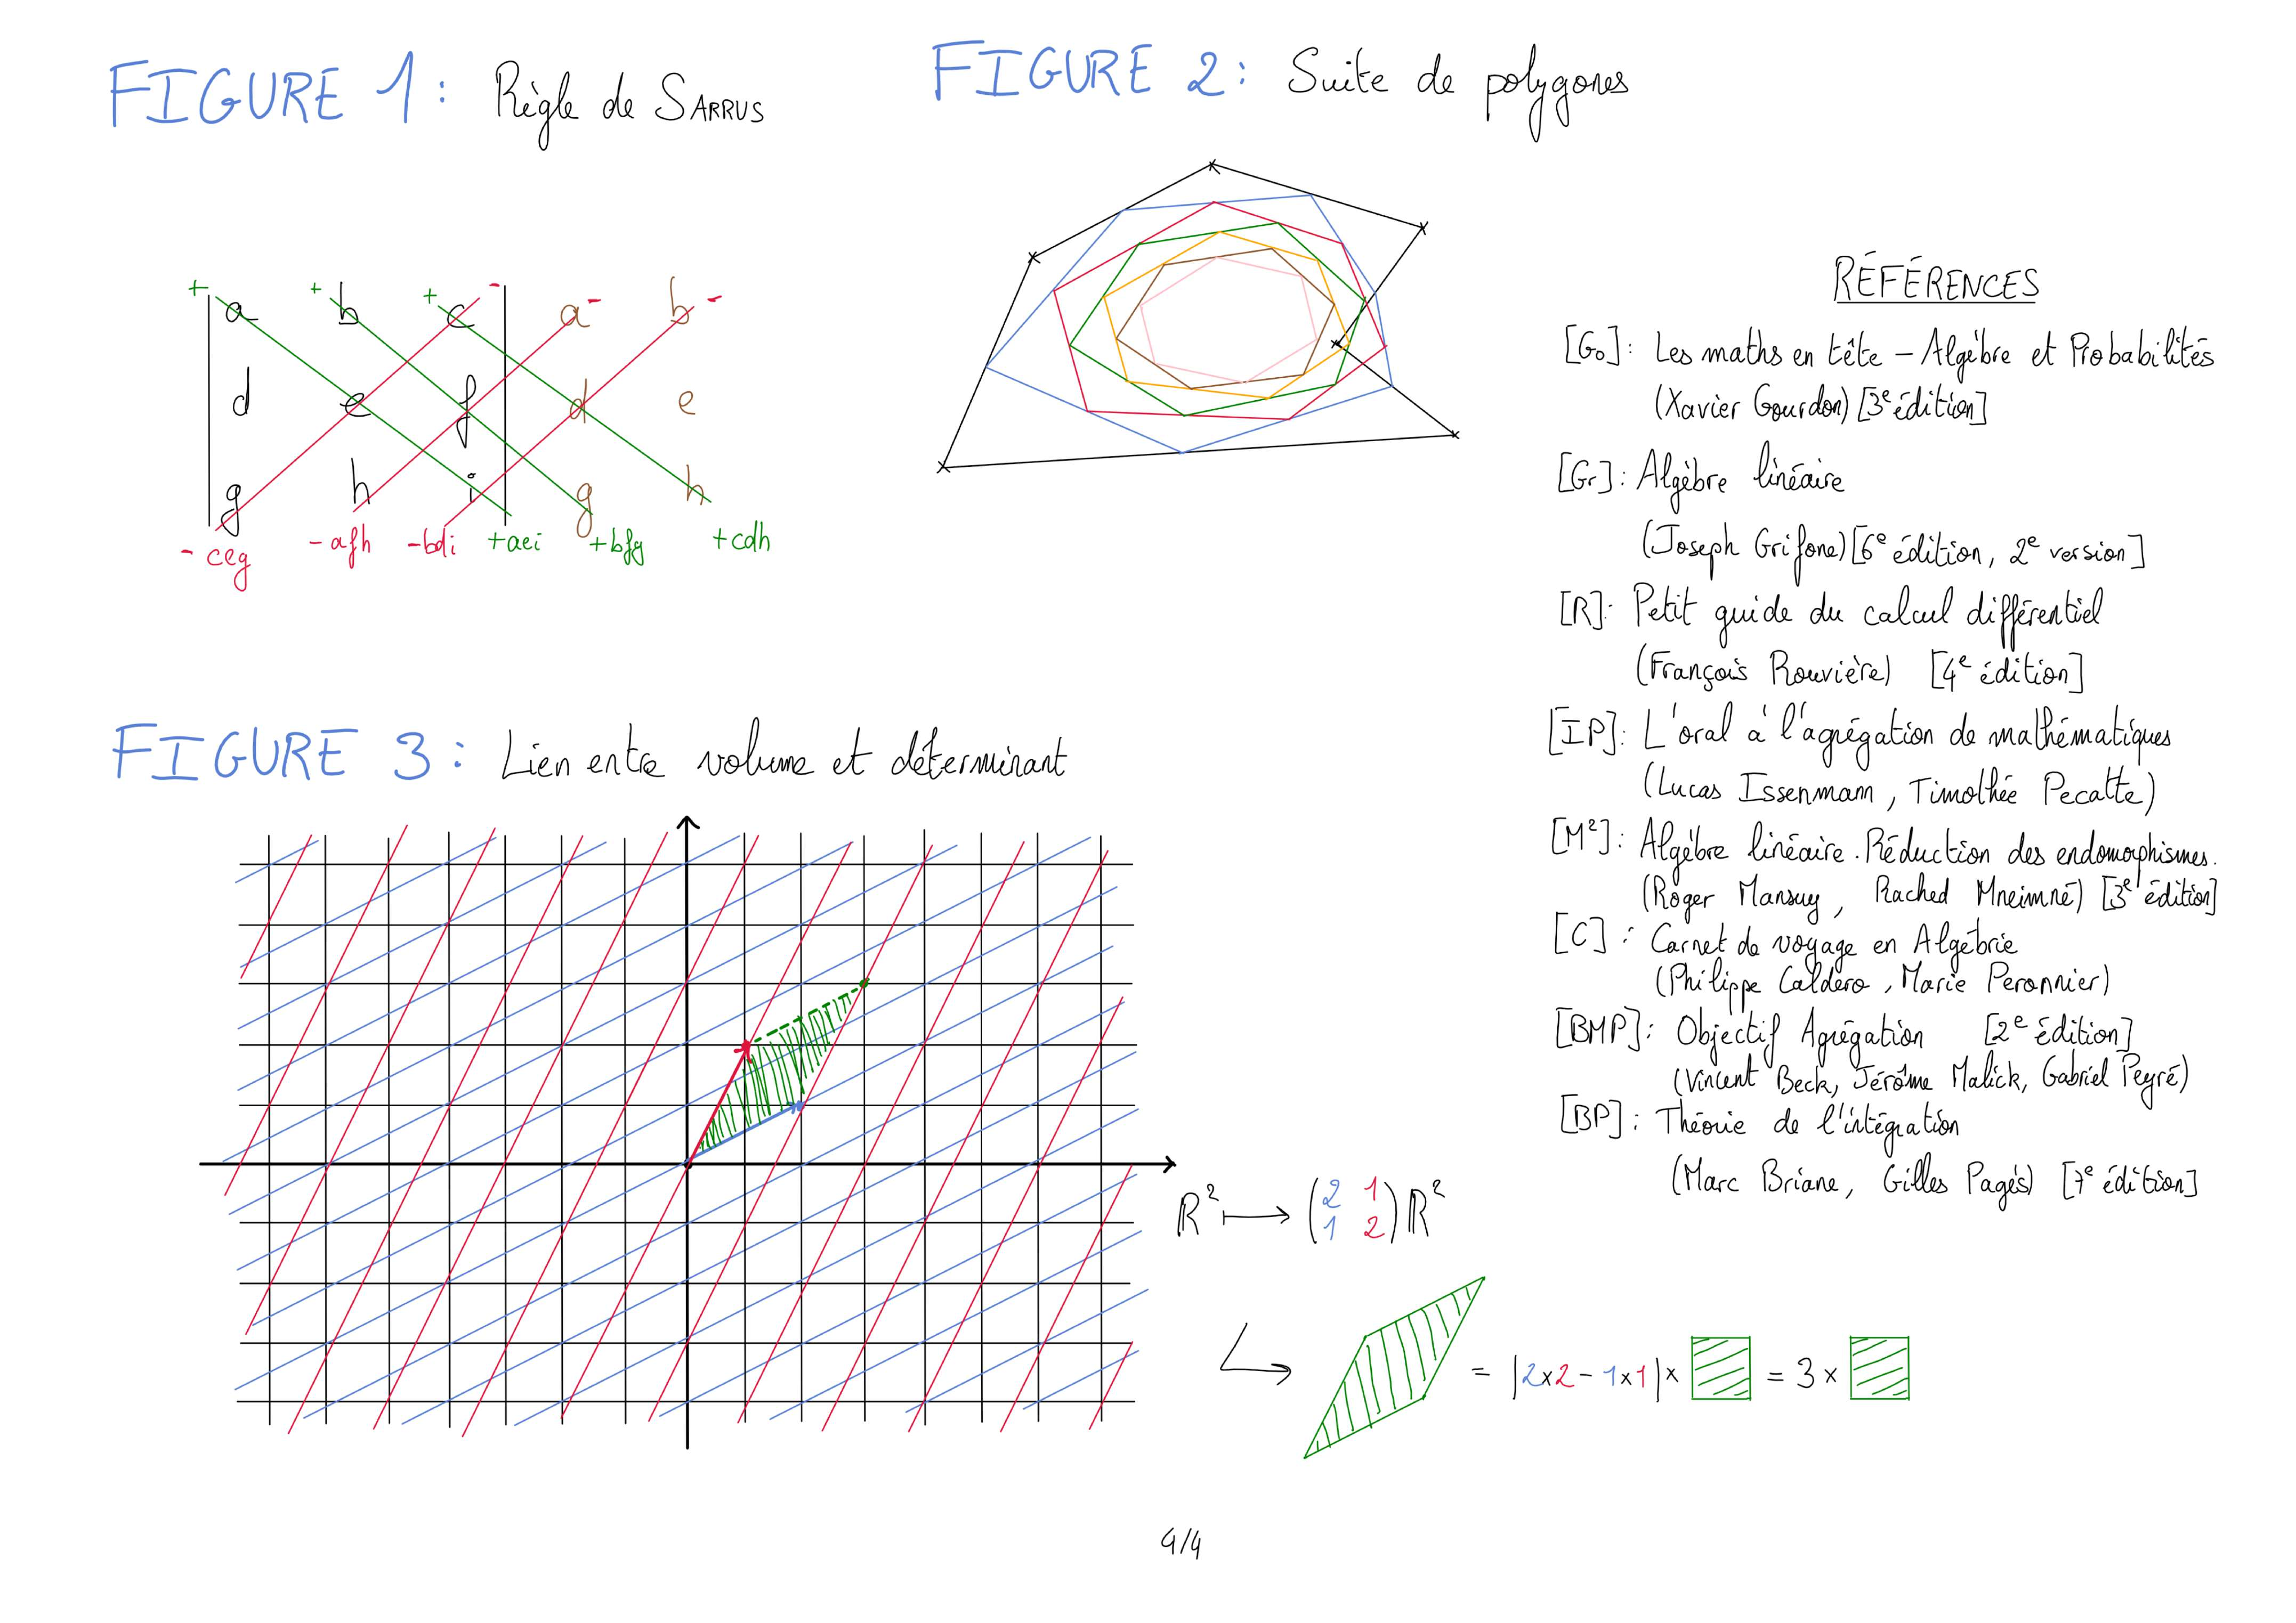
\includegraphics[trim={0 0 0 0},clip,width=1\linewidth]{img/149.pdf}
	\caption{s}
\end{figure}

\chapter*{151 : Sous-espaces stables par un endomorphisme ou une famille d'endomorphismes d'un espace vectoriel de dimension finie. Applications.}
\setcounter{definition}{0}

\textcolor{paragraphtext}{Soient $K$ un corps commutatif, $E$ un $K$-espace vectoriel de dimension $n\geq 1$ et $u\in\mathcal{L}(E)$. 
Soit $F$ un sous-espace vectoriel de $E$.}

\section*{I. Stabilité d'un sous-espace par un endomorphisme}
\subsection*{A. Introduction}

\begin{definition}[\textnormal{[M2] 17}]
	On dit que $F$ est \emph{stable par $u$} (ou \emph{$u$-stable}) si $u(F)\subseteq F$.
\end{definition}

\begin{example}[\textnormal{[M2] 17}]
	On a :
	\begin{itemize}
		\item $\left\{0\right\}$, $\Ker(u)$, $\im(u)$ et $E$ sont stables par $u$.
		\item $\forall P\in K[X]$, $\Ker(P(u))$ et $\im(P(u))$ sont stables par $u$.
	\end{itemize}
\end{example}

\begin{proposition}[\textnormal{[M2] 17}]
	Soit $v\in\mathcal{L}(E)$. Si $v$ commute avec $u$, alors pour tout $P\in K[X]$,
	$\Ker(P(u))$ et $\im(P(u))$ sont stables par $u$.
\end{proposition}

\begin{remark}
	En particulier, $\forall \lambda\in K$, $E_{\lambda}(u) := \Ker(u-\lambda \id_E)$ est 
	stable par $u$, et par tout endomorphisme qui commute avec $u$.
\end{remark}

\begin{proposition}[\textnormal{[M2] e17}]
	Soit $E = F\bigoplus G$ une décomposition de $E$, soit $\mathcal{B}$ une base de $E$ 
	adaptée à cette décomposition, notion $\Mat_{\mathcal{B}}(u) = \begin{pmatrix}
		A & B \\ C & D
	\end{pmatrix}$ par blocs. Alors $F$ (resp. $G$) est stable par $u$ si, et seulement si, $C=0$ (resp. $B = 0$).
\end{proposition}

\begin{corollary}[\textnormal{[M2] e120}]
	$F$ est stable par $u$ si, et seulement si, $F^{\perp}$ est stable par ${}^tu$.
	(NB : $\Mat_{\mathcal{B}^*}({}^t u) = {}^t\Mat_{\mathcal{B}}(u)$).
\end{corollary}

\subsection*{B. Notion d'endomorphisme induit}
\begin{definition}[\textnormal{[M2] 17}]
	Si $F$ est stabe par $u$, alors on dispose de \emph{l'endomorphisme induit par $u$ sur $F$} :
	$u_F\,\colon F\to F$, $x\mapsto u(x)$.
\end{definition}

\begin{proposition}[\textnormal{[M2] 55, 18}]
	Si $F$ est stable par $u$, alors $\chi_{u_F} \mid \chi_u$ et $\pi_{u_F}\mid \pi_u$.
\end{proposition}

\begin{corollary}[\textnormal{[M2] 93}]
	Si $F$ est stable par $u$ et si $u$ est diagonalisable (resp. trigonalisable, resp. nilpotent), alors $u_F$ aussi.
\end{corollary}

\begin{proposition}[\textnormal{[M2] 55, 18}]
	Si $E=F_1\bigoplus \cdots \bigoplus F_p$ est une décomposition de $E$ en somme de sous-espaces stables, alors :
	$\chi_u = \chi_{u_{F_1}}\cdots \chi_{u_{F_p}}$ et $\pi_u = \pi_{u_{F_1}}\vee \cdots \vee \pi_{u_{F_p}}$.
\end{proposition}

\section*{II. Application à la réduction des endomorphismes}

\begin{lemma}[des noyaux - \textnormal{[M2] 43}]
	$\forall (P,Q)\in K[X]^2$, $P\wedge Q = 1 \implies \Ker((PQ)(u)) = \Ker(P(u))\bigoplus \Ker(Q(u))$
\end{lemma}

\subsection*{A. Diagonalisation, trigonalisation}
\begin{theorem}[de \textsc{Cayley-Hamilton} - \textnormal{[M2] 82}]
	$\chi_u(u) = 0_{\mathcal{L}(E)}$
\end{theorem}

\begin{corollary}
	$E = \bigoplus_{\lambda\in \Sp(u)} \Ker\left(\left(u-\lambda \id_E\right)^{\mu_{\lambda_u}(\lambda)}\right)$
	est une décomposition de $E$ en somme de sous-espaces stables.
\end{corollary}

\begin{proposition}[\textnormal{[M2] 84}]
	Écrivons $\chi_u = \prod_{\lambda\in\Sp(u)} \left(X_\lambda\right)^{m(\lambda)}$
	et posons $E_{\lambda}(u)=\Ker(\lambda\id_E - u)$.
	Pour tout $\lambda\in \Sp(u)$, $1\leq \dim(E_{\lambda}(u))\leq m(\lambda)$.
\end{proposition}

\begin{theorem}[\textnormal{[R] 683; [M2] 90-93}]
	On a :
	\begin{itemize}
		\item $u$ est diagonalisable $\iff \pi_u$ est sciendé à racines simples $\iff$ il existe $P$ annulateur de $u$ sciendé à racines simples $\iff \chi_u$ est sciendé et $\forall\lambda\in\Sp(u)$, $\dim(E_{\lambda}(u)) = \mu_{\chi_u}(\lambda)$.
		\item $u$ est trigonalisable $\iff \chi_u$ est scindé $\iff$ il existe un polynôme scindé qui annule $u$.
	\end{itemize}
\end{theorem}

\begin{theorem}[de réduction simultanée - \textnormal{[M2] 94,107}]
	Soit $\left(u_i\right)_{i\in I}\in\mathcal{L}(E)^I$ une famille d'endomorphismes qui commutent deux à deux.
	Si tous les $u_i$, $i\in I$ sont diagonalisables (resp. trigonalisables), alors il existe une base de $E$ qui 
	diagonalise (resp. trigonalise) simultanément tous les $u_i$, $i\in I$.
\end{theorem}


\begin{tcolorbox}[
    breakable, % Allows the theorem to split across pages
    colback=developpement, % The background color
    colframe=gray!0!black, % The frame color
    boxrule=0pt, % The frame thickness
    arc=1mm, % Sharp corners
	boxsep=0pt,
	left=0pt, right=0pt, top=0pt, bottom=0pt
]
\begin{lemma}[\textnormal{[R] 743}]
	\label{151dev11}
	Il existe un sous-espace de $E$ de dimension $1$ ou $2$ stable par $u$.
\end{lemma}
\end{tcolorbox}

\subsection*{B. Cas des endomorphismes normaux}
\textcolor{paragraphtext}{Dans l'encadré suivant, on suppose $u$ normal}


\begin{tcolorbox}[
    breakable, % Allows the theorem to split across pages
    colback=developpement, % The background color
    colframe=gray!0!black, % The frame color
    boxrule=0pt, % The frame thickness
    arc=1mm, % Sharp corners
	boxsep=0pt,
	left=0pt, right=0pt, top=0pt, bottom=0pt
]
\begin{lemma}[\textnormal{[R] 743}]
	\label{151dev12}
	Si $F$ est un sous-espace de $E$ stable par $u$, alors $F^{\perp}$ est stable par $u$.
\end{lemma}
\begin{lemma}[\textnormal{[R] 744}]
	\label{151dev13}
	Il existe des sous-espaces $P_1,\dots, P_r$ de $E$ stables par $u$, de dimension $1$ ou $2$, deux à deux orthogonaux, tels que 
	$$E = P_1\bigoplus^{\perp}\cdots\bigoplus^{\perp} P_r$$
\end{lemma}
\end{tcolorbox}

\begin{lemma}[PAS DEV - \textnormal{[R] 745}]
	Si $n = \dim E = 2$, alors :
	\begin{itemize}
		\item Si $u$ admet une valeur propre réelle, alors $u$ est diagonalisable dans une base orthonormée,
		\item Sinon, pour toute base orthonormée $\mathcal{B}$ de $E$, il existe $(a,b)\in\IR^2$ tel que $b\neq 0$ et $\Mat_{\mathcal{B}}(u)=\begin{pmatrix}
			a & -b \\ b & a
		\end{pmatrix}$.
	\end{itemize}
\end{lemma}

\begin{tcolorbox}[
    breakable, % Allows the theorem to split across pages
    colback=developpement, % The background color
    colframe=gray!0!black, % The frame color
    boxrule=0pt, % The frame thickness
    arc=1mm, % Sharp corners
	boxsep=0pt,
	left=0pt, right=0pt, top=0pt, bottom=0pt
]
\begin{theorem}[de réduction des endomorphismes normaux - \textnormal{[R] 745}]
	Il existe une base orthonormée $\mathcal{B}$ de $E$ telle que, par blocs, $\Mat_{\mathcal{B}}(u) = \diag(D_p, R_1,\dots, R_r)$, où 
	$D_p\in\M_n(\IR)$ est diagonale, $\forall i\in \llbracket 1,n\rrbracket$, $\exists (a_i, b_i)\in\IR^2\,\colon b_i \neq 0$ et $R_i = \begin{pmatrix}
		a_i & -b_i \\ b_i & a_i
	\end{pmatrix}$ et $p+2r = n$.
\end{theorem}
\end{tcolorbox}

\begin{corollary}[théorème spectral - \textnormal{[R] 746 (734)}]
	Tout endomorphisme auto-adjoint se diagonalise dans une base orthonormée.
\end{corollary}

\begin{corollary}[\textnormal{[R] 727}]
	Si $u$ est orthogonal, alors il existe une base de $E$ dans laquelle la matrice de $u$ est de la forme, par blocs :
	$\begin{pmatrix}
		I_p & & & & \\
		& -I_q & & & \\
		& & R_1 & & \\
		& & & \ddots & \\
		& & & & R_r
	\end{pmatrix}$, où $R_k = \begin{pmatrix}
		\cos(\theta_k) & -\sin(\theta_k) \\ \sin(\theta_k) & \cos(\theta_k)
	\end{pmatrix}$
\end{corollary}

\begin{proposition}
	Si $u$ est une rotation et que $\dim (E)$ est impaire, alors $\Ker(u-\id_E)\neq \left\{0\right\}$.
\end{proposition}

\section*{II. Application à la décomposition des endomorphismes}
\subsection*{A. Décomposition de \textsc{Jordan} des endomorphismes nilpotents}

\begin{definition}[\textnormal{[M2] 143}]
	On appelle \emph{bloc de \textsc{Jordan}} de taille $d$ la matrice :
	$$J_d := \begin{pmatrix}
		0 & 1 & \cdots & 0 \\
		\vdots & \ddots & \ddots & \vdots \\
		\vdots & & \ddots & 1 \\
		0 & \cdots & \cdots & 0
	\end{pmatrix}$$

	Pour $\lambda = (\lambda_1, \dots, \lambda_r)\in\IN^r$, on pose $J_{\lambda} = \diag(J_{\lambda_1},\dots, J_{\lambda_r})$.
\end{definition}

\begin{theorem}[décomposition de \textsc{Jordan} des endomorphismes nilpotents - \textnormal{[M2] 144}]
	Supposons $u$ nilpotent d'indice $\lambda_1$.
	Il existe $\lambda_1 \geq \lambda_2 \geq \cdots \geq \lambda_r$
	telle que $\lambda_1 + \cdots + \lambda_r = n$, et $\mathcal{B}$ une base de $E$ telle que $\Mat_{\mathcal{B}}(u) = J_{\lambda_1,\dots,\lambda_r}$.
	Cette décomposition est unique.
\end{theorem}

\subsection*{B. Décomposition de \textsc{Dunford}}

\begin{theorem}[décomposition de \textsc{Dunford} - \textnormal{[M2] 141; [R] 613}]
	Si $u$ est trigonalisable, alors il existe un unique couple $(d,n)\in\mathcal{L}(E)^2$ tel que $u = d+n$, $d\circ n = n\circ d$, $d$ est diagonalisable et $n$ est nilpotent.
\end{theorem}

\begin{corollary}[\textnormal{[R] 634}]
	Sur $K =\IR$ ou $K=\IC$, $e^u$ est diagonalisable si, et seulement si, $u$ l'est.
\end{corollary}

\subsection*{C. Une application : le critère de diagonalisabilité de \textsc{Klarès}}

\begin{tcolorbox}[
    breakable, % Allows the theorem to split across pages
    colback=developpement, % The background color
    colframe=gray!0!black, % The frame color
    boxrule=0pt, % The frame thickness
    arc=1mm, % Sharp corners
	boxsep=0pt,
	left=0pt, right=0pt, top=0pt, bottom=0pt
]
\begin{theorem}[critère de \textsc{Klarès} - \textnormal{[M2] 154}]
	\label{151dev2}
	Posons $ad_u\,\colon v\in\mathcal{L}(E) \mapsto u\circ v - v\circ u$.
	Si $u$ est trigonalisable, alors :
	$$u \text{ diagonalisable} \iff \Ker(ad_u) = \Ker(ad_u^2)$$
\end{theorem}
\end{tcolorbox}

\section*{Développements}
\begin{itemize}
	\item Développement 1 : Lemmes \ref{151dev11}, \ref{151dev12}, \ref{151dev13} et Théorème \ref{151dev14}.
	\item Développement 2 : Théorème \ref{151dev2}
\end{itemize}

\section*{Références}
\begin{itemize}
	\item[R] \emph{Mathématiques pour l'agrégation - Algèbre et géométrie}, Jean-Étienne Rombaldi, 2e édition
	\item[M2] \emph{Algèbre linéaire. Réduction des endomorphismes}, Roger Mansuy, Rached Mneimné, 3e édition
\end{itemize}




\chapter*{155 : Exponentielle de matrices. Applications.}
\setcounter{definition}{0}

\textcolor{paragraphtext}{Dans cette leçon, $\IK$ désigne $\IR$ ou $\IC$, $n\in \IN^*$
et $(A,B)\in\M_n(\IK)^2$. On fixe une norme d'algèbre $\|\cdot\|$ sur $\M_n(\IK)$.
On suppose connu et maîtrisé le calcul matriciel élémentaire.}

\begin{theorem_def}[\textnormal{[R] 761}]
	La série $\sum_{k\in\IN} \frac{A^k}{k!}$ converge normalement sur 
	tout compact. Sa somme est appelée \emph{exponentielle de $A$}, et est notée $\exp(A)$ ou $e^A$.
\end{theorem_def}

\begin{example}[\textnormal{[R] 761}]
	$\forall (\lambda_1,\dots,\lambda_n)\in\IK^n$, $\exp(\diag(\lambda_1,\dots,\lambda_n)) = \diag(e^{\lambda_1},\dots,e^{\lambda_n})$.
	En particulier, $\exp(0_n) = I_n$ et $\exp(I_n) = e\cdot I_n$.
\end{example}

\begin{example}
	$\forall \theta\in\IR$, $R(\theta) := \begin{pmatrix}
		\cos(\theta) & -\sin(\theta) \\ \sin(\theta) & \cos(\theta)
	\end{pmatrix} = \exp\left(\begin{pmatrix}
		0 & -\theta \\ \theta & 0
	\end{pmatrix}\right)$
\end{example}

\section*{I. Propriétés algébriques de l'exponentielle matricielle}
\begin{proposition}
	Si $A$ et $B$ commutent, alors $\exp(A+B) = \exp(A)\exp(B)$.
	(NB : la réciproque est vraie !) et $\exp(A)$ et $\exp(B)$ commutent.
\end{proposition}

\begin{cexample}
	$A = \begin{pmatrix}
		1 & 0 \\ 0 & -1
	\end{pmatrix}$ et $B = \begin{pmatrix}
		0&1\\0&0
	\end{pmatrix}$ ne commutent pas, et $e^A e^B = \begin{pmatrix}
		e&e\\0& 1/e
	\end{pmatrix} \neq \begin{pmatrix}
		e & 1/e \\ 0 & 1/e
	\end{pmatrix} = e^B e^A$.
\end{cexample}

\begin{corollary}
	$\exp(\M_n(\IK)) \subseteq GL_n(\IK)$, et $\exp(A)^{-1} = \exp(-A)$.
\end{corollary}

\begin{proposition}[\textnormal{[R] 761-762}]
	On a les propriétés suivantes :
	\begin{itemize}
		\item $\forall P\in GL_n(\IK)$, $P\exp(A)P^{-1}=\exp(PAP^{-1})$
		\item ${}^t\exp(A) = \exp({}^tA)$
		\item $\det(\exp(A)) = e^{\tr(A)}$
		\item $\overline{\exp(A)} = \exp(\overline{A})$
	\end{itemize}
\end{proposition}

\begin{corollary}
	$\exp(\mathcal{A}_n(\IK)) \subseteq O_n(\IK)$, avec $\mathcal{A}_n(\IK) = \left\{M\in\M_n(\IK)\mid {}^tM = -M\right\}$.
\end{corollary}

\begin{remark}
	On peut montrer que $\exp(\mathcal{A}_n(\IR)) = SO_n(\IR)$.
\end{remark}

\begin{proposition}
	Si $A$ est diagonalisable, alors $\Sp(\exp(A)) = \exp(\Sp(A))$.
\end{proposition}

\begin{theorem}
	On a :
	\begin{itemize}
		\item $\exp(A)\in \IK_{n-1}[A]$ et commute avec $A$.
		\item Si $A$ est diagonalisable et $\IK = \IR$, alors $A\in \IR_{n-1}[\exp(A)]$.
	\end{itemize}
\end{theorem}

\begin{remark}
	Pour $A = \begin{pmatrix}
		0&0\\0& 2i\pi
	\end{pmatrix}\in\M_2(\IC)$, on a $\exp(A) = I_2$ donc pour tout $P\in \IC[X]$, $P(\exp(A)) = P(1)I_2 \neq A$.
\end{remark}

\section*{II. L'exponentielle d'une matrice en pratique}
\subsection*{A. Quelques méthodes de calcul}

\begin{proposition}
	Supposons $A$ diagonalisable. Il existe $(\lambda_1,\dots, \lambda_n)\in\IK^n$ et $P\in O_n(\IK)$ tels que 
	$A = P\begin{pmatrix}
		\lambda_1 & & \\
		& \ddots & \\
		& & \lambda_n
	\end{pmatrix}P^{-1}$; alors $\exp(A) = P\begin{pmatrix}
		e^{\lambda_1} & & \\ & \ddots & \\ & & e^{\lambda_n}
	\end{pmatrix}P^{-1}$.
\end{proposition}

\begin{theorem}[décomposition de \textsc{Dunford} - \textnormal{[R] 613}]
	Si $A$ est trigonalisable, alors il existe un unique $(D,B)\in \M_n(\IK)^2$ tel que $D$ est diagonalisable, $N$ est nilpotente, $D$ et $N$ commutents, et $A = D+N$.
	De plus, $(D,N)\in K[A]^2$.
\end{theorem}

\begin{proposition}
	Si $A$ est nilpotente d'indice $r$, alors $\exp(A) = \sum_{k=0}^{r-1} \frac{A^k}{k!}$.
\end{proposition}

\begin{proposition}[\textnormal{[R] 765}]
	Si $A$ est trigonalisable, et si $A=D+N$ est la décomposition de \textsc{Dunford} de $A$,
	alors $e^A = e^D + e^D(e^N-I_n)$.

	En particulier, $e^D$ est diagonalisable et $e^D(e^N -I_n)$ est nilpotente, et ce sont les éléments de la décomposition de \textsc{Dunford} de $e^A$.
\end{proposition}

\begin{proposition}[\textnormal{[R] 778}]
	$\left(I_n + \frac{A}{k}\right)^k \to_{k\to +\infty} \exp(A)$
\end{proposition}

\begin{remark}
	Cela fournit une méthode pour approcher numériquement l'exponentielle d'une matrice, toutefois bien moins efficace qu'un calcul direct.
\end{remark}

\subsection*{B. Application : résolution d'EDO linéaires à coéfficients constants}
\begin{proposition}[\textnormal{[Gr] 378}]
	$t\mapsto e^{tA}$ est lisse sur $\IR$, de dérivée $t\mapsto Ae^{tA} = e^{tA}A$.
\end{proposition}

\begin{proposition}[\textnormal{[Gr] e378}]
	L'unique solution du problème de \textsc{Cauchy}
	$$\begin{cases}
		Y' = AY \\ Y(t_0) = Y_0
	\end{cases}$$
	pour $t_0\in \IR$, $Y\in\M_{n,1}(\IR)$, est $t\mapsto e^{(t-t_0)A}Y_0$.
\end{proposition}

\begin{example}
	Le problème de \textsc{Cauchy}
	$\begin{cases}
		Y' = \begin{pmatrix}
			1&1\\0&1
		\end{pmatrix}Y,\quad Y(0) = \begin{pmatrix}
			0\\1
		\end{pmatrix}
	\end{cases}$
	admet pour (unique) solution $t\mapsto \exp\left(t\begin{pmatrix}
		1&1\\0&1
	\end{pmatrix}\right)\begin{pmatrix}
		0\\1
	\end{pmatrix} = e^t\begin{pmatrix}
		1&t\\0&1
	\end{pmatrix}\begin{pmatrix}
		0\\1
	\end{pmatrix} = e^t\begin{pmatrix}
		t\\1
	\end{pmatrix}$.
\end{example}

\begin{proposition}[formule de \textsc{Duhamel}]
	Soient $B\,\colon \IR\to \M_{n,1}{\IR}$ continue, $t_0\in\IR$ et $Y_0\in\M_{n,1}(\IR)$.
	L'unique solution du problème de \textsc{Cauchy}
	$\begin{cases}
		Y' = AY + B ;\quad Y(t_0) = Y_0
	\end{cases}$ est 
	$$t\mapsto e^{(t-t_0)A}Y_0 + \int_{t_0}^t e^{(t-s)A}B(s)ds$$
\end{proposition}


\section*{III. Propriétés analytiques de l'exponentielle matricielle}
\subsection*{A. Injectivité, surjectivité}

\begin{theorem}[\textnormal{[R] 769}]
	L'application $\exp\,\colon \M_n(\IC)\to GL_n(\IC)$ est surjective, non injective.
\end{theorem}

\begin{cexample}
	$\forall k\in\IZ$, $\exp(2i\pi kI_n)= I_n$
\end{cexample}

\begin{theorem}
	L'application $\exp\,\colon \M_n(\IR)\to GL_n(\IR)$ n'est ni surjective, ni injective.
	Plus précisément,
	\begin{itemize}
		\item $\exp(\M_n(\IR)) = \left\{M^2 \mid M\in GL_n(\IR)\right\} \neq GL_n(\IR)$
		\item Exemple 3 justifie la non-injectivité
	\end{itemize}
\end{theorem}

\begin{remark}
	Comme $\det(\exp(A)) = e^{\tr (A)} > 0$, on a $\det^{-1}(\IR^-)\cap \exp(\M_n(\IR)) = \emptyset$.
\end{remark}

\begin{proposition}[\textnormal{[R] e768-777}]
	Notons $\mathcal{N}_n(\IR)$ l'ensemble des matrices nilpotentes de $\M_n(\IR)$.
	L'application $\exp\,\colon \mathcal{N}_n(\IR) \to GL_n(\IR)$ est injective.

	Notons $\Delta_n(\IR)$ l'ensemble des matrices diagonalisables de $\M_n(\IR)$.
	L'application $\exp\,\colon \Delta_n(\IR)\to  GL_n(\IR)$ est injective.
\end{proposition}

\begin{application}[\textnormal{[R] 777}]
	$\exp(A)$ est diagonalisable si, et seulement si, $A$ l'est.
\end{application}


\begin{tcolorbox}[
    breakable, % Allows the theorem to split across pages
    colback=developpement, % The background color
    colframe=gray!0!black, % The frame color
    boxrule=0pt, % The frame thickness
    arc=1mm, % Sharp corners
	boxsep=0pt,
	left=0pt, right=0pt, top=0pt, bottom=0pt
]
\begin{theorem}[\textnormal{[C] 357}]
	\label{155dev1}
	L'application $\exp\,\colon S_n(\IR)\to S_n^{++}(\IR)$ est un homéomorphisme.
\end{theorem}
\end{tcolorbox}

\begin{theorem_def}[\textnormal{[R] 766-768}]
	Si $A\in \mathcal{B}(I_n, 1)$, alors $\sum_{n\geq 1}\left(-1\right)^{n-1}\frac{A^n}{n}$
	converge normalement sur tout compact. Sa somme est notée $\ln(I_n+A)$, et est appelée \emph{logarithme de $A$}.
\end{theorem_def}

\begin{remark}
	On a $\ln(I_n) = 0_n$.
\end{remark}

\begin{theorem}[ADMIS]
	L'application $\exp\,\colon \mathcal{N}_n(\IC)\to I_n + \mathcal{N}_n(\IC)$ est une 
	bijection de réciproque $\ln$.
\end{theorem}

\subsection*{B. Régularité}
\begin{theorem}[ADMIS - \textnormal{[Rv] 306}]
	$\exp$ est lisse sur $\M_n(\IR)$.
\end{theorem}

\begin{tcolorbox}[
    breakable, % Allows the theorem to split across pages
    colback=developpement, % The background color
    colframe=gray!0!black, % The frame color
    boxrule=0pt, % The frame thickness
    arc=1mm, % Sharp corners
	boxsep=0pt,
	left=0pt, right=0pt, top=0pt, bottom=0pt
]
\begin{proposition}
	\label{155dev2}
	La différentielle de $\exp$ en $X\in\M_n(\IR)$ est :
	$$d(\exp)(X)\,\colon H\mapsto \left(\sum_{n=0}^{+\infty}\frac{[\cdot, X]^n}{(n+1)!}\right)(H)$$
	où $[\cdot, X]\,\colon H \mapsto [H, X] = HX - XH$.
\end{proposition}
\end{tcolorbox}

\begin{corollary}
	$\exp$ induit un $C^1$-difféomorphisme local d'un voisinage de $0_n$ sur un voisinage de $I_n$.
\end{corollary}

\section*{Développements}
\begin{itemize}
	\item Développement 1 : Théorème \ref{155dev1}
	\item Développement 2 : Proposition \ref{155dev2}
\end{itemize}

\section*{Références}
\begin{itemize}
	\item[R] \emph{Mathématiques pour l'agrégation - Algèbre et géométrie}, Jean-Étienne Rombaldi, 2e édition
	\item[C] \emph{Nouvelles histoires hédonistes de groupes et géométries I}, P. Caldero, J. Germoni
	\item[Gr] \emph{Algèbre linéaire}, Joseph Grifone, 6e édition, 2e version
	\item[Rv] \emph{Petit guide du calcul différentiel}, François Rouvière, 4e édition
\end{itemize}


\chapter*{156 : Endomorphismes trigonalisables. Endomorphismes nilpotents.}
\setcounter{definition}{0}
\textcolor{paragraphtext}{Dans cette leçon, $K$ désigne un corps, $E$ est un $K$-espace vectoriel de dimension finie $n$, et $u\in\mathcal{L}(E)$.}

\section*{I. Rappels sur l'étude des endomorphismes}

\begin{theorem}[de structure - \textnormal{[M2] 2}]
	L'application $\varphi_u\,\colon K[X]\to \mathcal{L}(E)$ qui à 
	$P = \sum a_kX^k$ associe $P(u) := \sum a_k u^k$, est un morphisme de $K$-algèbres.
\end{theorem}

\begin{proposition_def}[\textnormal{[M2] 3,4}]
	L'ensemble $I_u = \Ker(\varphi_u)$ des polynômes dits \emph{annulateurs de $u$}, est un idéal de $K[X]$,
	appelé \emph{idéal annulateur de $u$}. Il n'est pas réduit à $\left\{0\right\}$, et 
	donc admet un unique générateur unitaire, noté $\mu_u$, appelé \emph{polynôme minimal de $u$}.
\end{proposition_def}

\begin{remark}
	Par correspondance entre $\mathcal{L}(E)$ et $\M_n(K)$, ces résultats restent valables pour les matrices.
\end{remark}

\begin{definition}[\textnormal{[M2] 54}]
	Le \emph{polynôme caractéristique de $u$} est définie par $\chi_u = \det(X\id_E - u)$.
\end{definition}

\begin{theorem}[de \textsc{Cayley-Hamilton} - \textnormal{[M2] 81}]
	$\chi_u(u) = 0_{\mathcal{L}(E)}$
\end{theorem}

\begin{proposition}[\textnormal{[R] 605}]
	$\Sp(u) = \chi^{-1}(\left\{0\right\}) = \pi^{-1}(\left\{0\right\})$
\end{proposition}

\begin{proposition}[\textnormal{[M2] 55 ?}]
	Soit $F$ un sous-espace vectoriel de $E$ stable par $u$.
	Notons $u_F\in\mathcal{L}(E)$ l'nedomorphisme induit par $u$ sur $F$. Alors $\pi_{u_F} \mid \pi_u$ et $\chi_{u_F} \mid \chi_u$.
\end{proposition}

\begin{proposition}[\textnormal{[M2] 18-55}]
	Si $E = F_1\bigoplus \cdots\bigoplus F_r$ est une décomposition de $E$ en sous-espaces stables par $u$,
	alors $\chi_u = \chi_{u_{F_1}} \cdots \chi_{u_{F_r}}$ et $\pi_u = \pi_{u_{F_1}} \vee \cdots \vee \pi_{u_{F_r}}$.
\end{proposition}

\begin{lemma}[des noyaux - \textnormal{[M2] 43}]
	Soit $(P,Q)\in K[X]^2$. Si $P\wedge Q = 1$, alors
	$\Ker\left(\left(PQ\right)(u)\right) = \Ker(P(u))\bigoplus\Ker(Q(u))$.
\end{lemma}

\section*{II. Trigonalisation}

\begin{definition}[\textnormal{[R] 675}]
	On dit que $u$ est \emph{trigonalisable} s'il existe une base $\mathcal{B}$ de $E$ telle que $\Mat_{\mathcal{B}}(u)$ est triangulaire.
\end{definition}

\begin{corollary}[\textnormal{[R] 676}]
	Si $u$ est trigonalisable, alors $\tr(u) = \sum_{\lambda\in\Sp(u)} m(\lambda)\lambda$ et $\det(u) = \prod_{\lambda\in\Sp(u)} \lambda^{m(\lambda)}$.
\end{corollary}

\begin{theorem}[\textnormal{[R] 676}]
	$u$ est trigonalisable $\iff$ $\pi_u$ est scindé $\iff$ il existe $P\in I_u$ scindé.
\end{theorem}

\begin{corollary}[\textnormal{[R] 676}]
	Sur un corps algébriquement clos, tout endomorphisme est trigonalisable.
\end{corollary}

\begin{example}
	$\begin{pmatrix}
		0&1\\-1&0
	\end{pmatrix}$ est trigonalisable sur $\IC$ mais pas sur $\IR$.
\end{example}

\begin{application}[\textnormal{[R] 762}]
	$\forall A\in \M_n(\IC)$, $\det(e^A) = e^{\tr(A)}$.
\end{application}

\begin{proposition}
	Si $F$ est un sous-espace vectoriel stable par $u$ et si $u$ est trigonalisable, alors $u_f\,\colon F\to F$ est trigonalisable.
\end{proposition}

\begin{proposition}
	Si $A\in\M_n(K)$ s'écrit par blocs $\diag(A_1,\dots,A_r)$,
	alors $\chi_A = \chi_{A_1}\cdots \chi_{A_r}$ et $\pi_A = \pi_{A_1}\vee \cdots \vee \pi_{A_r}$.
\end{proposition}

\begin{proposition}[\textnormal{[Go] 175}]
	Soit $v\in \mathcal{L}(E)$. Si $u$ et $v$ commutent, alors popur tout $\lambda\in\Sp(u)$, $E_{\lambda}(u)$ est stable par $v$.
\end{proposition}

\begin{theorem}[\textnormal{[R] 678}]
	Soit $\left(u_i\right)_{i\in I}\in\mathcal{L}(E)^I$ une famille d'endomorphismes qui commutent deux à deux. Si les $u_i$, $i\in I$, sont tous trigonalisables, alors ils le sont dans une même base (on dit qu'ils sont \emph{cotrigonalisables}).
\end{theorem}

\begin{proposition}[\textnormal{[Go] e192}]
	Soit $v\in\mathcal{L}(E)$. Si $u$ et $v$ sont cotrigonalisables, alors $u+v$ et $u\circ v$ sont trigonalisables.
\end{proposition}

\begin{example}
	On a :
	\begin{itemize}
		\item $\left(\begin{smallmatrix}
			0& -1\\ 0 & 0
		\end{smallmatrix}\right)$ et $\left(\begin{smallmatrix}
			0& 1\\ 0 & 0
		\end{smallmatrix}\right)$ sont trigonalisables, mais pas leur somme.
		\item $\left(\begin{smallmatrix}
			0& 1\\ 1 & 0
		\end{smallmatrix}\right)$ et $\left(\begin{smallmatrix}
			1 & 1\\ 0 & -1
		\end{smallmatrix}\right)$ sont trigonalisables, mais pas leur produit.
	\end{itemize}
\end{example}

\section*{III. Endomorphismes nilpotents}
\subsection*{A. Définition, critères, propriétés}

\begin{definition}[\textnormal{[Gr] 93}]
	On dit que $u$ est \emph{nilpotent} s'il existe $k\in\IN^*$ tel que $u^k=0_{\mathcal{L}(E)}$.
	On définit alors \emph{l'indice (de nilpotence) de $u$} comme $\min\left\{k\in\IN^*\mid u^k = 0_{\mathcal{L}(e)}\right\}$.
\end{definition}

\begin{example}
	La dérivation de $\IC_n[X]$ est nilpotente d'indice $n+1$.
\end{example}

\begin{proposition}[\textnormal{[Gr] e192}]
	Soit $v\in\mathcal{L}(E)$ nilpotent. Si $u$ et $v$ commutent, alors $u+v$ et $u\circ v$ sont nilpotents.
\end{proposition}

\begin{theorem}
	Les assertions suivantes sont équivalentes :
	\begin{itemize}
		\item $u$ est nilpotent
		\item $\chi_u = X^n$
		\item $\exists k\in \llbracket 1,n\rrbracket$, $\pi_u = X^p$
		\item $u$ est trigonalisable et $\Sp(u) = \left\{0\right\}$.
	\end{itemize}
\end{theorem}

\begin{corollary}
	Si $K$ est algébriquement clos, alors $u$ est nilpotent $\iff \Sp(u)=\left\{0\right\}$. 
\end{corollary}

\begin{example}
	$\left(\begin{smallmatrix}
		0&0&0\\ 0&0&-1 \\ 0&1&0
	\end{smallmatrix}\right)$ n'est pas nilpotente, mais son spectre est $\left\{0\right\}$.
\end{example}

\begin{theorem}[\textnormal{[C] 27-32}]
	Si $K=\IR$, alors $u$ est nilpotent $\iff$ $\forall k\in \IN^*$, $\tr(u^k) = 0$.
\end{theorem}

\begin{remark}
	Si $K$ est un corps fini, le résultat est faux : considérer $\id_{\left(\IF_p\right)^p}$.
\end{remark}

\begin{proposition}
	Si $F$ est un sous-espace vectoriel stable par $u$ et si $u$ est nilpotent, alors $u_F\,\colon F\to F$ est nilpotent.
\end{proposition}

\subsection*{B. Réduction de \textsc{Jordan} des endomorphismes nilpotents}

\begin{notation}[\textnormal{[M2] 143}]
	Posons $$J_r := \begin{pmatrix}
		0 & 1 & \cdots & 0 \\
		\vdots & \ddots & \ddots & \vdots \\
		\vdots & & \ddots & 1 \\
		0 & \cdots & \cdots & 0
	\end{pmatrix}$$

	On l'appelle \emph{bloc de \textsc{Jordan}} d'ordre $r$.
\end{notation}

\begin{lemma}[\textnormal{[R] 678}]
	Supposons $u$ nilpotent d'indice $p$. Soit $x\notin \Ker(u^{p-1})$, posons $F_x = \Vect(x, u(x), \dots, u^{p-1}(x))$.
	\begin{itemize}
		\item $F_x$ est stable par $u$ et $(x,u(x),\dots,u^{p-1}(x))$ est une base de $F_x$ ;
		\item $F_x$ admet un supllémentaire stable par $u$.
	\end{itemize}
\end{lemma}

\begin{theorem}[réduction de \textsc{Jordan}]
	Supposons $u$ nilpotent. Il existe $d_1\geq \cdots\geq d_r$ et une base $\mathcal{B}$ de $E$ tels que $\Mat_{\mathcal{B}}(u) = \diag(J_{d_1},\dots,J_{d_r})$.
\end{theorem}

\begin{proposition}
	Posons $A = \diag(J_{i_1},\dots,J_{i_r})$. On a $\chi_A = \pi_A = X^{i_r}$, et $A$ est nilpotente d'indice $r$.
\end{proposition}

\subsection*{C. Noyaux itérés et tableaux de \textsc{Young}}

\begin{proposition}[\textnormal{[M2] 16}]
	La suite $\left(\Ker(u^k)\right)_{k\in\IN}$ est croissante et stationnaire, et si on note $d_k = \dim(\Ker(u^k))$, on a $\forall k\in \IN$, $d_{k+1} = d_k + \dim(\Ker(u)\cap \im(u^k))$.
\end{proposition}

\begin{proposition}[\textnormal{[M2] 16}]
	$\left(d_{k+1}-d_k\right)_{k\in\IN}$ est décroissante (on dit que $\left(d_k\right)_{k\in\IN}$ \emph{s'essouffle}).
\end{proposition}

\begin{proposition}[\textnormal{[Gr] 93}]
	$p=\min\left\{k\in \IN\mid \forall q\geq k,\, \Ker(u^q)=\Ker(u^k)\right\}$ est appelé \emph{caractère de $u$}.
	Il vérifie $p\leq n$. Si $u$ est nilpotent, alors $p$ est aussi l'indice de nilpotence de $u$.
\end{proposition}

\begin{definition}[\textnormal{[M2] 147}]
	\begin{itemize}
		\item Le \emph{tableau de \textsc{Young}} associé à une suite d'entiers $n_1\geq \cdots \geq n_r$ est le tableau à $r$ lignes tel que la $i$-ième ligne contient $n_i$ cases (alignées à gauche).
		\item Le \emph{tableau de \textsc{Young}} d'un endomorphisme nilpotent est le tableau de \textsc{Young} de $d_2-d_1\geq d_3-d2\geq \cdots \geq d_p - d_{p-1}$ avec les notations ci-dessus.
	\end{itemize}
\end{definition}

\begin{example}
	FIGURE 1.
\end{example}

\begin{proposition}
	Soit $d_1\geq \cdots\geq d_r$. La matrice par blocs $\diag(J_{d_1},\dots,J_{d_r})$ est nilpotente d'indice $d_1$.
\end{proposition}

\begin{example*}[Construction du tableau de \textsc{Young} à partir de la réduite de \textsc{Jordan}]
	[\textnormal{[M2] 147}]
	FIGURE 2. A PRESENTER.
\end{example*}

\begin{theorem}[\textnormal{[M2] 148}]
	Deux endomorphismes nilpotents sont semblables si, et seulement si, ils ont la même réduction de \textsc{Jordan}.
\end{theorem}

\begin{corollary}
	Il y a autant de classes de similitude de matrices nilpotentes que de partitions de $n$.
\end{corollary}


\section*{IV. Décomposition de \textsc{Dunford} et applications}
\textcolor{paragraphtext}{Dans cette section, $\IK$ désigne $\IR$ ou $\IC$.}


\begin{tcolorbox}[
    breakable, % Allows the theorem to split across pages
    colback=developpement, % The background color
    colframe=gray!0!black, % The frame color
    boxrule=0pt, % The frame thickness
    arc=1mm, % Sharp corners
	boxsep=0pt,
	left=0pt, right=0pt, top=0pt, bottom=0pt
]
\begin{theorem}[décomposition de \textsc{Dunford} - \textnormal{[R] 683}]
	\label{156dev11}
	Si $\chi_u$ est scindé, alors il existe un unique $(d,n)\in\mathcal{L}(E)^2$ tel que $d$ est diagonalisable, $n$ nilpotent, $d$ et $n$ commutent et $u = d + n$.
	De plus, $(d,n)\in K[u]^2$.
\end{theorem}

\begin{application}[\textnormal{[R] 684}]
	\label{156dev12}
	Soit $A\in\M_n(\IK)$ tel que $\chi_A$ est scindé. Soit $A = D+N$ sa
	décomposition de \textsc{Dunford}. Il existe $P\in GL_n(\IK)$ et $(\lambda_1,\dots,\lambda_n)\in\IK^n$ tels que 
	$P^{-1}DP = \diag(\lambda_1,\dots, \lambda_n)$. On a alors :
	$$e^A = P\diag(e^{\lambda_1},\dots, e^{\lambda_n})P^{-1}\sum_{k=0}^{n-1}\frac{N^k}{k!}$$
\end{application}
\end{tcolorbox}

\begin{example}
	$\exp\left(\begin{smallmatrix}
		1&1&0\\0&1&1\\0&0&1
	\end{smallmatrix}\right) = \exp\left(I_3 + J_3\right) = \left(\begin{smallmatrix}
		e&e&e/2 \\ 0&e&e \\ 0&0&0
	\end{smallmatrix}\right)$
\end{example}

\begin{application}
	$\left\{Y\in C^1(\IR,\IK^n)\mid Y' = AY\right\} = \left\{t\mapsto e^{tA}Y_0\mid Y_0\in \IK^n\right\}$
\end{application}


\begin{tcolorbox}[
    breakable, % Allows the theorem to split across pages
    colback=developpement, % The background color
    colframe=gray!0!black, % The frame color
    boxrule=0pt, % The frame thickness
    arc=1mm, % Sharp corners
	boxsep=0pt,
	left=0pt, right=0pt, top=0pt, bottom=0pt
]
\begin{theorem}[critère de \textsc{Klarès} - \textnormal{[M2 154]}]
	\label{156dev2}
	Si $u\in \mathcal{L}(E)$ est trigonalisable, alors $u$ est diagonalisable si, et seulement si, $ad_u\,\colon v\in\mathcal{L}(E)\mapsto u\circ v - v\circ u$ l'est.
\end{theorem}
\end{tcolorbox}

\section*{Développements}
\begin{itemize}
	\item Développement 1 : Théorème \ref{156dev11} et application \ref{156dev12}
	\item Développement 2 : Théorème \ref{156dev2}
\end{itemize}

\section*{Références}
\begin{itemize}
	\item[Gr] \emph{Algèbre linéaire}, Joseph Grifone, 6e édition, 2e version
	\item[M2] \emph{Algèbre linéaire. Réduction des endomorphismes}, Roger Mansuy, Rached Mneimné, 3e édition
	\item[R] \emph{Mathématiques pour l'agrégation - Algèbre et géométrie}, Jean-Étienne Rombaldi, 2e édition
	\item[Go] \emph{Les maths en tête - Algèbre et probabilités}, Xavier Gourdon, 3e édition
	\item[C] \emph{Carnet de voyage en Algébrie}, Philippe Caldero, Marie Peronnier
\end{itemize}
\begin{figure}[!htb]
	\centering
	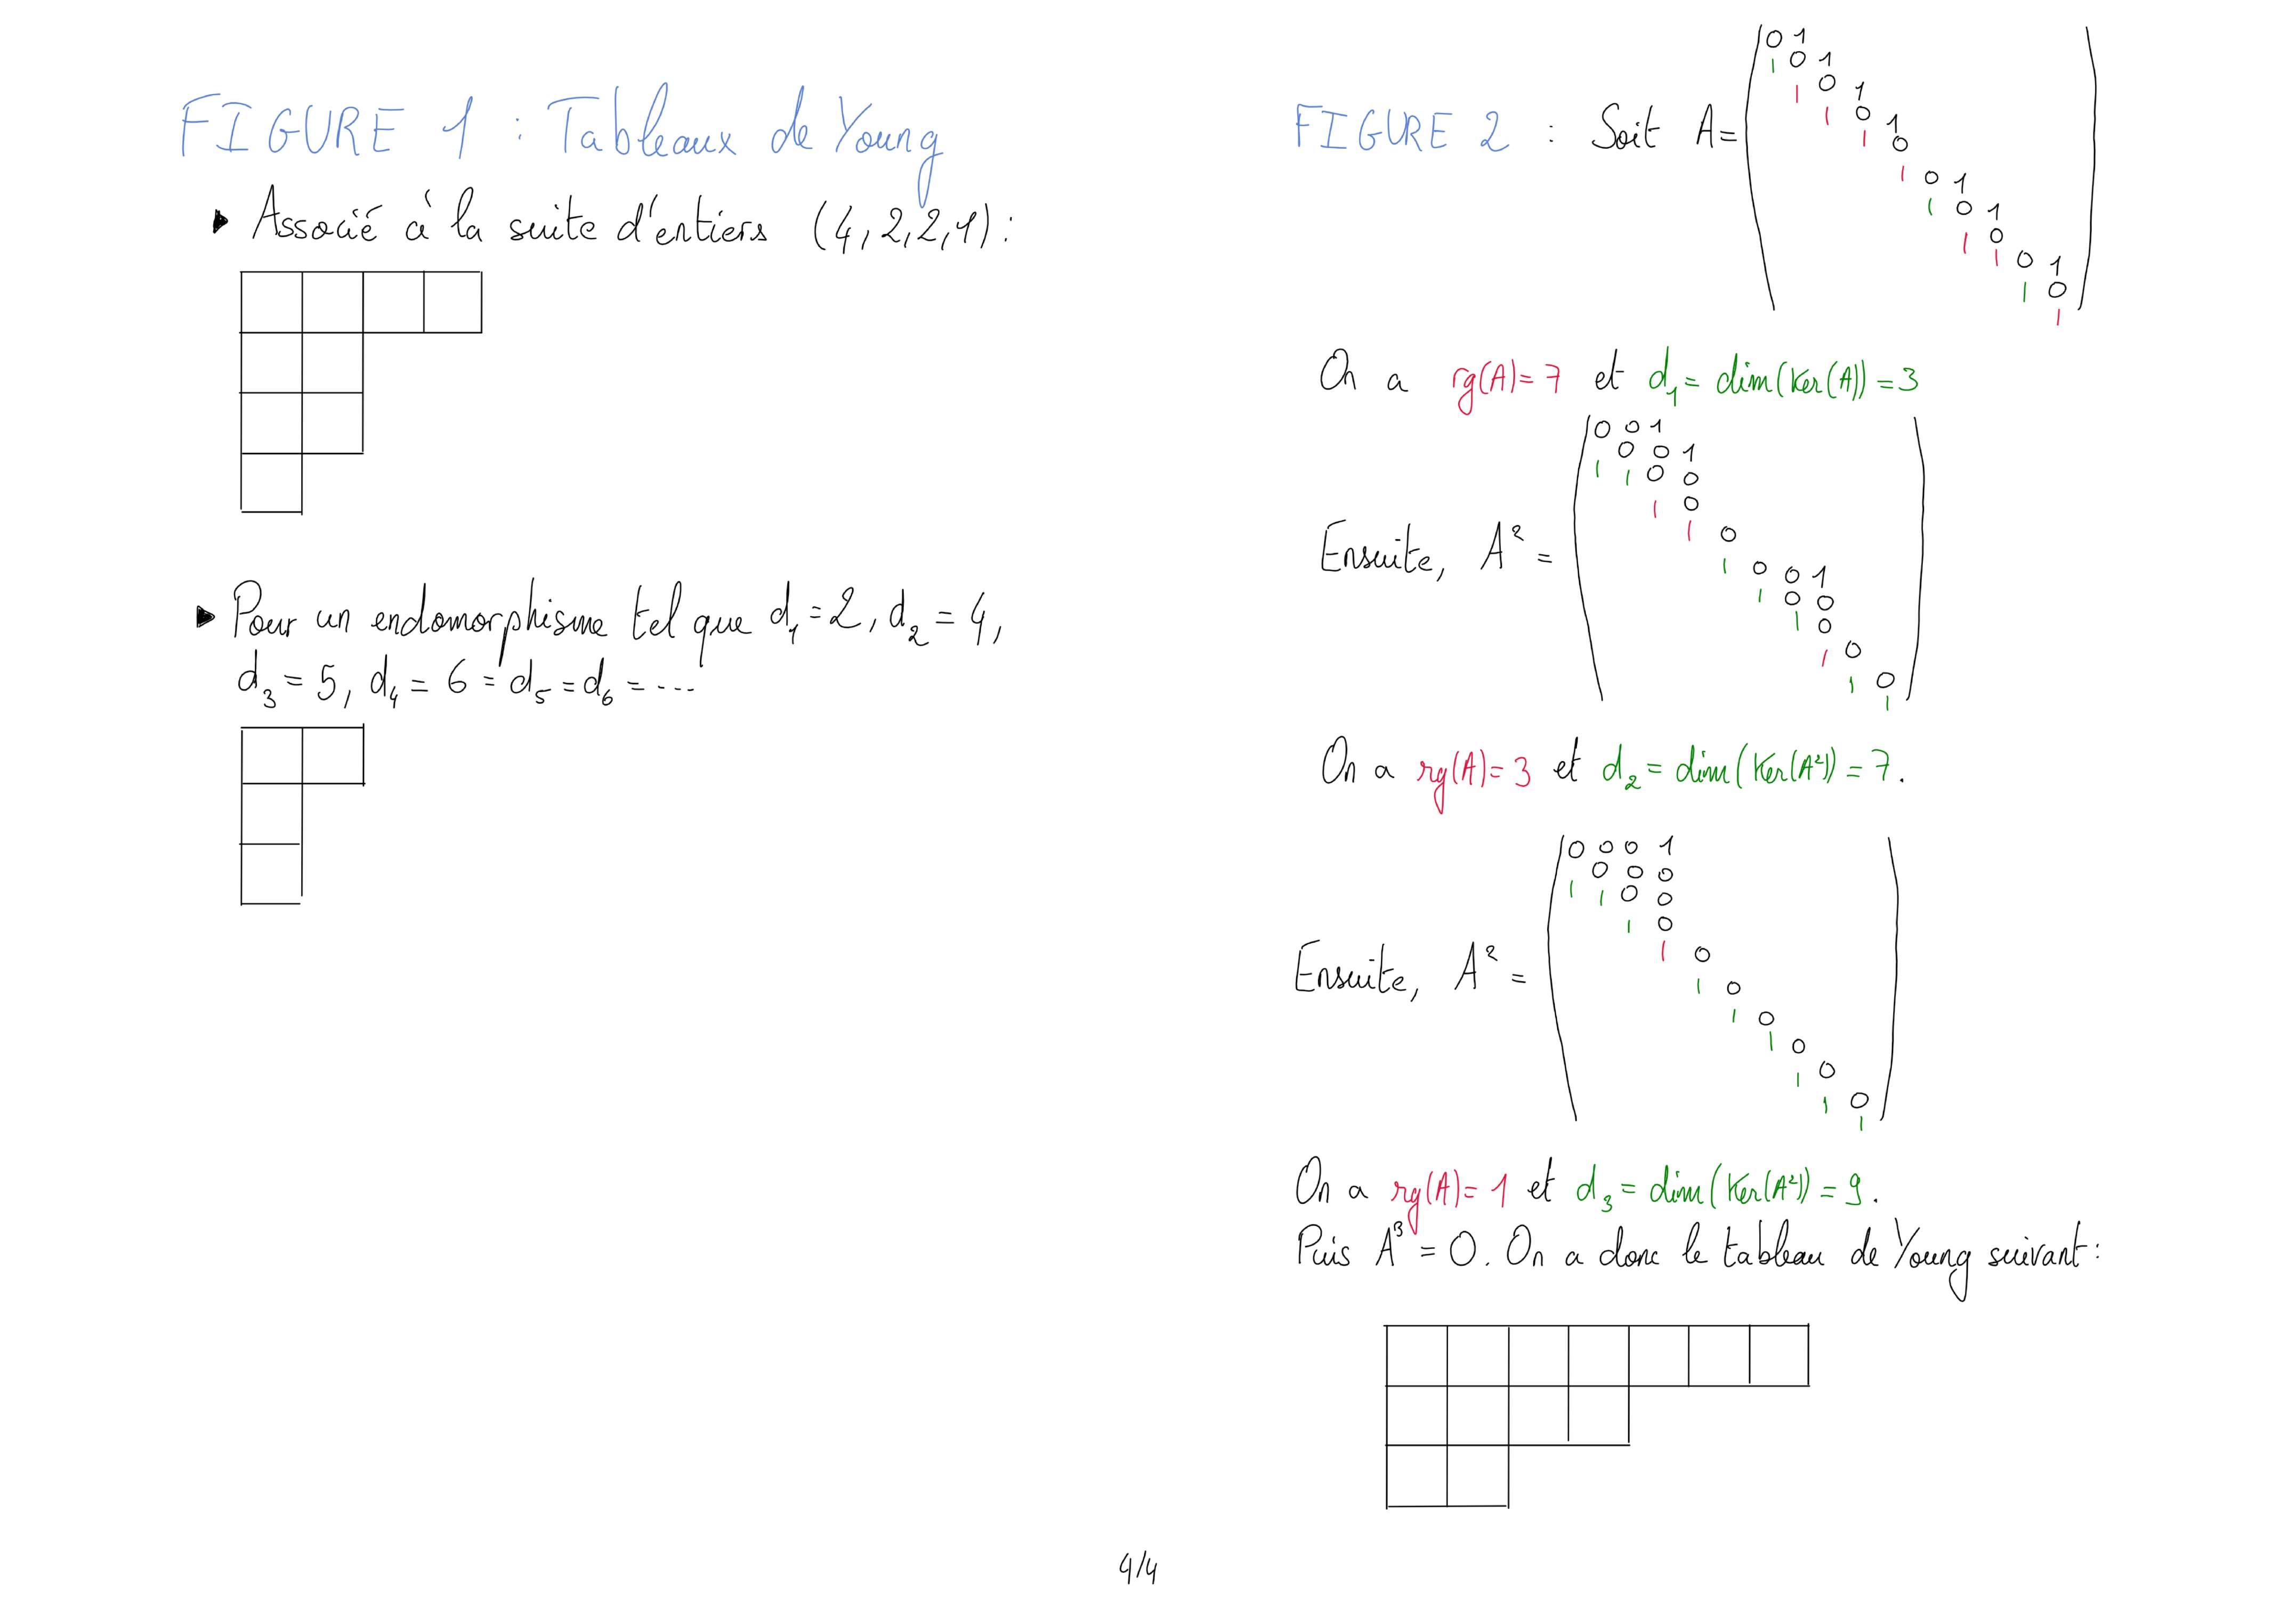
\includegraphics[trim={0 0 0 0},clip,width=1\linewidth]{img/156.pdf}
	\caption{s}
\end{figure}

\chapter*{157 : Matrices symétriques réelles, matrices hermitiennes.}
\setcounter{definition}{0}
\textcolor{paragraphtext}{Dans cette leçon, $\IK$ désigne $\IR$ ou $\IC$.
On fixe $n\in\IN^*$. Pour $A\in \M_n(\IK)$, on pose $A^*={}^t\overline{A}$.
Soient $E$ un $\IK$-espace vectoriel de dimension finie $n$, soit $\B=\left\{e_1,\dots,e_n\right\}$
une base de $E$.}

\section*{I. Généralités}
\subsection*{A. Définitions et premières propriétés}

\begin{definition}[\textnormal{[Go] 240-241}]
	On définit :
	\begin{itemize}
		\item $\mathcal{S}_n(\IR) = \left\{A\in\M_n(\IR)\mid {}^tA=A\right\}$ est l'ensemble des matrices réelles dites \emph{symétriques} ;
		\item $\A_n(\IR) = \left\{A\in\M_n(\IR)\mid {}^tA=-A\right\}$ est l'ensemble des matrices réelles dites \emph{anti-symétriques} ;
		\item $\mathcal{H}_n(\IR) = \left\{A\in\M_n(\IC)\mid {}^t\overline{A} = A\right\}$ est l'ensemble des matrices complexes dites \emph{hermitiennes} ;
		\item On dit que $A$ est \emph{auto-adjointe} si $A=A^*$, \emph{i.e.} si $A\in \mathcal{S}_n(\IR)$ ou $A\in\mathcal{H}_n(\IC)$.
	\end{itemize}
\end{definition}

\begin{example}
	$\left(\begin{smallmatrix}
		0&1\\1&0
	\end{smallmatrix}\right)\in\mathcal{S}_2(\IR)$ et 
	$\left(\begin{smallmatrix}
		0&-i\\i&1
	\end{smallmatrix}\right)\in\mathcal{H}_2(\IC)$.
\end{example}

\begin{proposition}[\textnormal{[Go] 240-241}]
	$\M_n(\IR) = \mathcal{S}_n(\IR)\bigoplus\A_n(\IR)$
	et $\M_n(\IC) = \mathcal{S}_n(\IC)\bigoplus i\A_n(\IR)$.
\end{proposition}

\begin{definition}
	On définit :
	\begin{itemize}
		\item $\mathcal{S}_n^+(\IR) = \left\{A\in\mathcal{S}_n(\IR)\mid \forall X\in\IRn,\,{}^tXAX \geq 0\right\}$ est l'ensemble des matrices symétriques réelles dites \emph{positives}.
		\item $\mathcal{S}_n^{++}(\IR) = \left\{A\in\mathcal{S}_n^+(\IR)\mid \forall X\in\IRn,\,{}^tXAX = 0\implies X=0\right\}$ l'ensemble des matrices symétriques réelles dites \emph{définies positives}.
		\item $\mathcal{H}_n^+(\IC) = \left\{A\in\mathcal{H}_n(\IC)\mid \forall X\in\IC^n,\,{}^t\overline{X}AX \geq 0\right\}$ est l'ensemble des matrices hermitiennes dites \emph{positives}.
		\item $\mathcal{H}_n^{++}(\IC) = \left\{A\in\mathcal{H}_n(\IC)\mid \forall X\in\IC^n,\,{}^t\overline{X}AX = 0\implies X=0\right\}$ est l'ensemble des matrices hermitiennes dites \emph{définies positives}.
	\end{itemize}
\end{definition}

\subsection*{B. Lien avec les formes quadratiques / hermitiennes}

\begin{definition}[\textnormal{[Go] 240-241}]
	Soit $\varphi\,\colon E^2\to \IR$ une forme bilinéaire. On dit que $\varphi$ est \emph{symétrique} si 
	$\forall(x,y)\in E^2,\, \varphi(x,y)=\varphi(y,x)$. Le cas échéant, $q\,\colon x\in E \mapsto \varphi(x,x)$ est appelée \emph{forme quadratique associée à $\varphi$},
	et $\varphi$ est appelée \emph{forme polaire associée à $q$} (elle est alors unique).
\end{definition}

\begin{definition}
	Soit $\varphi\,\colon E^2\to\IC$ une forme sesquilinéaire (on prend l'antilinéarité à droite).
	On dit que $\varphi$ est \emph{hermitienne} si $\forall(x,y)\in E^2,\,\varphi(x,y)=\overline{\varphi(y,x)}$.
	Le cas échéant, $q\,\colon x\in E\mapsto \varphi(x,x)$ est appelée \emph{forme hermitienne associée à $\varphi$}, et $\varphi$ est appelée \emph{forme polaire associée à $q$} (elle est alors unique).
\end{definition}

\begin{example}[\textnormal{[Go] 239}]
	\begin{itemize}
		\item $(f,g)\mapsto\int_{0}^{1}f\overline{g}$ est une forme sesquilinéaire hermitienne sur $C^0([0,1],\IC)$, et induit une forme bilinéaire symétrique sur $C^0([0,1],\IR)$.
		\item $(X,Y)\mapsto {}^t\overline{X}Y$ est bilinéaire symétrique ou sesquilinéaire hermitienne sur $\IK^n$.
	\end{itemize}
\end{example}

\begin{proposition}[\textnormal{[Go] e241}]
	Soit $\varphi\,\colon E^2\to \IK$ bilinéaire ou sesquilinéaire. On définit la \emph{matrice de $\varphi$ dans $\B$} comme $\Mat_{\B}(\varphi):= \left(\varphi(e_i,e_j)\right)_{i,j}$.
	Pour $x$ et $y$ dans $E$, de vecteurs coordonées $X$ et $Y$, on a alors $\varphi(x,y)={}^t\overline{X}\cdot \Mat_{\B}(\varphi)\cdot Y$ en identifiant $\IK$ et $\M_{n,1}(\IK)$.
	Alors, 
	\begin{itemize}
		\item $\varphi$ est symétrique si, et seulement si, $\Mat_{\B}(\varphi)\in \mathcal{S}_n(\IR)$
		\item $\varphi$ est hermitienne si, et seulement si, $\Mat_{\B}(\varphi)\in \mathcal{H}_n(\IC)$
	\end{itemize}
\end{proposition}

\begin{proposition}[\textnormal{[R] 163}]
	Soit $\B'$ une autre base de $E$. Si $P$ est la matrice de passage de $\B$ à $\B'$, alors $\Mat_{\B'}(\varphi)={}^t\overline{P}AP$.
\end{proposition}

\begin{proposition}
	$\forall A\in\mathcal{S}_n(\IR)\cup \mathcal{H}_n(\IC)$, $\Sp(A)\subseteq \IR$.
\end{proposition}

\section*{II. Réduction des matrices symétriques / hermitiennes}
\subsection*{A. Orthogonalité et théorème spectral}
\textcolor{paragraphtext}{Soit $q$ une forme quadratique ou hermitienne sur $E$, de forme polaire $\varphi$. On pose $A =\Mat_{\B}(\varphi)$.}

\begin{definition}[\textnormal{[Go] 243}]
	On dit que $\B$ est \emph{$q$-orthogonale} si $\forall(i,j)\in\llbracket 1,n\rrbracket$, $i\neq j\implies \varphi(e_i, e_j) = 0$, \emph{i.e.} si $A$ est diagonale.
\end{definition}


\begin{tcolorbox}[
    breakable, % Allows the theorem to split across pages
    colback=developpement, % The background color
    colframe=gray!0!black, % The frame color
    boxrule=0pt, % The frame thickness
    arc=1mm, % Sharp corners
	boxsep=0pt,
	left=0pt, right=0pt, top=0pt, bottom=0pt
]
\begin{theorem}[spectral - \textnormal{[Go] 256}]
	\label{157dev11}
	Pour toute $M\in\mathcal{S}_n(\IR)$ (resp. $M\in\mathcal{H}_n(\IC)$),
	il existe $P$ orthogonale (resp. unitaire) (\emph{i.e.} $P^{-1} = P^*$) telle que $P^*MP$ est diagonale.
\end{theorem}
\begin{theorem}[\textnormal{[Go] 243}]
	\label{157dev12}
	Il existe une base $q$-orthogonale de $E$.
\end{theorem}
\end{tcolorbox}

\begin{application}
	Soit $A\in\mathcal{S}_n(\IR)$. Alors :
	\begin{itemize}
		\item $A\in\mathcal{S}_n^+(\IR)\iff \Sp(A)\subseteq \IR^+$ ;
		\item $A\in\mathcal{S}_n^{++}(\IR) \iff \Sp(A)\subseteq \IR^{+*}$
	\end{itemize}
\end{application}

\begin{tcolorbox}[
    breakable, % Allows the theorem to split across pages
    colback=developpement, % The background color
    colframe=gray!0!black, % The frame color
    boxrule=0pt, % The frame thickness
    arc=1mm, % Sharp corners
	boxsep=0pt,
	left=0pt, right=0pt, top=0pt, bottom=0pt
]
\begin{theorem}
	\label{157dev13}
	$\forall A\in \mathcal{S}_n^{++}(\IR)$, $\forall B\in \mathcal{S}_n(\IR)$, $\exists P\in GL_n(\IR)$ tels que 
	${}^tPAP=I_n$ et ${}^tPBP$ est diagonale.
\end{theorem}
\end{tcolorbox}

\begin{theorem}
	$\forall A\in \mathcal{S}_n^+(\IR)$, $\exists ! B\in\mathcal{S}_n^+(\IR)$ : $A=B^2$ (on note $B = \sqrt{A}$).
\end{theorem}

\begin{theorem}[décomposition polaire - \textnormal{[C] 348}]
	Toute matrice $A$ (inversible) se décompose (de manière unique)
	sous la forme $A=\Theta S$, où $\Theta\in \mathcal{O}_n(\IR)$ et $S\in\mathcal{S}_n^{++}(\IR)$.
\end{theorem}

\subsection*{B. Réduction de \textsc{Gauss} et signature d'une forme quadratique / hermitienne}

\begin{theorem}[réduction de \textsc{Gauss} - \textnormal{[R] 469}]
	Il existe des formes linéaires $l_1,\dots, l_r$ linéairement indépendantes et $(\lambda_1,\dots,\lambda_n)\in\IK^r$ tels que $q = \lambda_1 \vert l_1\vert^2 + \dots + \lambda_r \vert l_r\vert^2$.
\end{theorem}

\begin{example}
	\label{157ex19}
	$q(x,y,z) = x^2+2xy-yz+\frac{3}{q}z^2=(x+y)^2 -(y+\frac{1}{2})^2 + z^2$
\end{example}

\begin{theorem}[loi d'inertie de \textsc{Sylvester} - \textnormal{[R] 477}]
	Supposons que $\IK = \IR$, soit $\B=(e_1,\dots,e_n)$ une base $q$-orthogonale de $E$.
	Les entiers $s = \#\left\{e_i\in\B \mid q(e_i)> 0\right\}$ et $t = \#\left\{e_i\in\B\mid q(e_i)<0\right\}$
	ne dépendent que de $q$. Le couple $(s,t)$ est appelé \emph{signature de $q$}.
\end{theorem}

\begin{example}
	La forme quadratique de l'exemple \ref{157ex19} a pour signature $(2,1)$.
\end{example}

\begin{corollary}[\textnormal{[R] 207}]
	Les orbites de l'action de $GL_n(\IR)$ sur $\mathcal{S}_n(\IR)$ par congruence sont caractérisées par le rang et la signature.
\end{corollary}

\section*{III. Propriétés topologiques en lien avec $\mathcal{S}_n(\IR)$}

\begin{definition}
	Pour $A\in\M_n(\IK)$, on pose $\exp(A)=\sum_{k=0}^{+\infty} \frac{A^k}{k!}$.
\end{definition}

\begin{example}
	$\forall (\lambda_1,\dots,\lambda_n)\in\IK^n$, $\exp(\diag(\lambda_1,\dots,\lambda_n)) = \diag(e^{\lambda_1},\dots, e^{\lambda_n})$.
\end{example}


\begin{tcolorbox}[
    breakable, % Allows the theorem to split across pages
    colback=developpement, % The background color
    colframe=gray!0!black, % The frame color
    boxrule=0pt, % The frame thickness
    arc=1mm, % Sharp corners
	boxsep=0pt,
	left=0pt, right=0pt, top=0pt, bottom=0pt
]
\begin{theorem}[\textnormal{[C] 357}]
	\label{157dev2}
	On a que $\exp\,\colon \mathcal{S}_n(\IR)\to \mathcal{S}_n^{++}(\IR)$ est un homéomorphisme.
\end{theorem}
\end{tcolorbox}

\section*{IV. Applications}
\subsection*{A. Vecteurs gaussiens}

\textcolor{paragraphtext}{Soit $(\Omega,\A,\IP)$ un espace probabilisé. On note $\langle\cdot\mid\cdot\rangle$ le produit scalaire canonique sur $\IR^n$.}

\begin{definition}[\textnormal{[CR] 160,157,158}]
	Un vecteur aléatoire $X=(X_1,\dots, X_n)\,\colon (\Omega,\A,\IP)\to (\IR^n,\B(\IR^n))$ est un \emph{vecteur gaussien} si pour tout $u\in\IR^n$, $\langle u\mid X\rangle$
	suit une loi normale (réelle). On note alors $X\sim \mathcal{N}_n(m,\Gamma)$ où $m = {}^t(\IE[X_1],\dots, \IE[X_n])$ est l'espérance de $X$, 
	et $\Gamma = \left(\Cov(X_i,X_j)\right)_{1\leq i,j\leq n}\in\mathcal{S}_n^+(\IR)$ sa matrice de covariance.
\end{definition}

\begin{example}[\textnormal{[CR] 160}]
	Si $X_1,\dots,X_n$ sont indépendantes de loi $\mathcal{N}(0,1)$, alors $\begin{pmatrix}
		X_1 \\ \vdots \\ X_n
	\end{pmatrix}\sim \mathcal{N}(0_n, I_n)$.
\end{example}

\begin{theorem}[\textnormal{[CR] 160}]
	Une variable aléatoire $X$ est gaussienne si, et seulement s'il existe $m\in\IR^m$ et $\Gamma\in\mathcal{S}_n^+(\IR)$ tels que :
	$$\forall u\in\IR^n,\,\varphi_X(u) = \exp(i\langle m,u\rangle - \frac{1}{2}\langle\Gamma u, u\rangle)$$

	Le cas échéant, $m$ est l'espérance, et $\Gamma$ sa matrice de covariance.
\end{theorem}

\begin{corollary}
	La loi d'un vecteur gaussien est entièrement déterminée par son espérance et sa matrice de covariance.
\end{corollary}

\begin{proposition}[\textnormal{[CR] 161}]
	Si $X\sim \mathcal{N}_n(m,\Gamma)$, alors $\forall A\in\M_{p,n}(\IR),\,\forall b\in\IR^p,\, AX+b\sim \mathcal{N}_p(Am+b, A\Gamma {}^tA)$.
\end{proposition}

\begin{proposition}
	$\forall\Gamma\in \mathcal{S}_n^{++}(\IR),\,\exists c\in\M_n(\IR)$ tels que $\Gamma = {}^tCC$.
\end{proposition}

\begin{corollary}[\textnormal{[CR] 161}]
	Pour tous $m\in\IR^n$ et $\Gamma\in\mathcal{S}_n(\IR)$, il existe un vecteur gaussien de loi $\mathcal{N}_n(m,\Gamma)$.
\end{corollary}

\begin{theorem}
	Soient $m\in\IR^n$, $\Gamma\in\mathcal{S}_n^+(\IR)$ et $X\sim\mathcal{N}_n(m,\Gamma)$.
	Alors $X$ est à densité $\iff$ $\Gamma\in\mathcal{S}_n^{++}(\IR)$.
	
	Le cas échéant, $\forall u\in \IR^n$, $f_X(u) = \left(2\pi\right)^{-\frac{n}{2}}\det(\Gamma)^{-\frac{1}{2}}\exp\left(-\frac{1}{2}\langle\Gamma^{-1}(u-m)\mid u-m\rangle\right)$.
\end{theorem}

\subsection*{B. Optimisation des fonctions de plusieurs variables}

\textcolor{paragraphtext}{Soit $f\,\colon \IR^n\to \IR$ de classe $C^2$.}

\begin{definition}[\textnormal{[Rv] 294}]
	On appelle \emph{(matrice) hessien de $f$ en $a$} la matrice $\Hess_a(f) = \left(\frac{\partial^2 f}{\partial e_i\partial e_j}(a)\right)_{1\leq i,j\leq n}$.
\end{definition}

\begin{remark}
	$\Hess_a(f)$ est la matrice dans $\B$ de la forme bilinéaire $d^2f(a)$ : en particulier, pour tous $h = \begin{pmatrix}
		h_1 \\ \vdots \\ h_n
	\end{pmatrix}\in \IR^n$, $d^2f(a)(h)(k) = {}^th\cdot\Hess_a(f)\cdot k$.
\end{remark}

\begin{definition}[\textnormal{[Go] 336}]
	On dit que $a$ est un \emph{point critique} si $df(a)=0$.
\end{definition}

\begin{theorem}[\textnormal{[Go] 335-336}]
	Si $f$ admet un maximum (resp. un minimum) local en $a$, alors $a$ est un point critique, et $\Hess_a(f)$ est négative (resp. positive).

	NB : la réciproque est vraie si on suppose en plus $\Hess_a(f)$ définie.
\end{theorem}

\begin{algorithm}[de descente de gradient à pas fixe]
	Soient $\Omega$ un ouvert de $\IR^n$, $f\in C^1(\Omega, \Omega)$, $\alpha > 0$ et $x_0\in\Omega$.
	La suite définie par $\forall n\in\IN$, $x_{n+1} = x_n - \alpha\nabla f(x_n)$ converge vers un $x^*\in\Omega$ vérifiant $\nabla f(x^*)$.
\end{algorithm}

\begin{theorem}[\textnormal{[BMP] 24-32}]
	Soient $A\in\mathcal{S}_n^{++}(\IR)$ et $b\in\IR^n$.
	La solution de $Ax=b$ est donné par le minimum de $x\mapsto \frac{1}{2}\langle Ax, x\rangle - \langle b,x\rangle$, lequel peut être trouvé par descente de gradient.
\end{theorem}



\section*{Développements}
\begin{itemize}
	\item Développement 1 : Partie 1) Théorèmes \ref{157dev11} et \ref{157dev12}; Partie 2) Théorème \ref{157dev13}
	\item Développement 2 : Théorème \ref{157dev2}
\end{itemize}

\section*{Références}
\begin{itemize}
	\item[R] \emph{Mathématiques pour l'agrégation - Algèbre et géométrie}, Jean-Étienne Rombaldi, 2e édition
	\item[Go] \emph{Les maths en tête - Algèbre et probabilités}, Xavier Gourdon, 3e édition
	\item[C] \emph{Carnet de voyage en Algébrie}, Philippe Caldero, Marie Peronnier
	\item[CR] \emph{Probabilités et statistiques pour l'épreuve de modélisation à l'agrégation de mathématiques}, Marie-Line Chabanol, Jean-Jacques Ruch
	\item[Rv] \emph{Petit guide du calcul différentiel}, François Rouvière, 4e édition
	\item[BMP] \emph{Objectif Agrégation}, Vincent Beck, Jérôme Malick, Gabriel Peyré, 2e édition
\end{itemize}

\chapter*{159 : Formes linéaires et dualité en dimension finie. Exemples et applications.}
\setcounter{definition}{0}

% \begin{figure}[!htb]
% 	\centering
% 	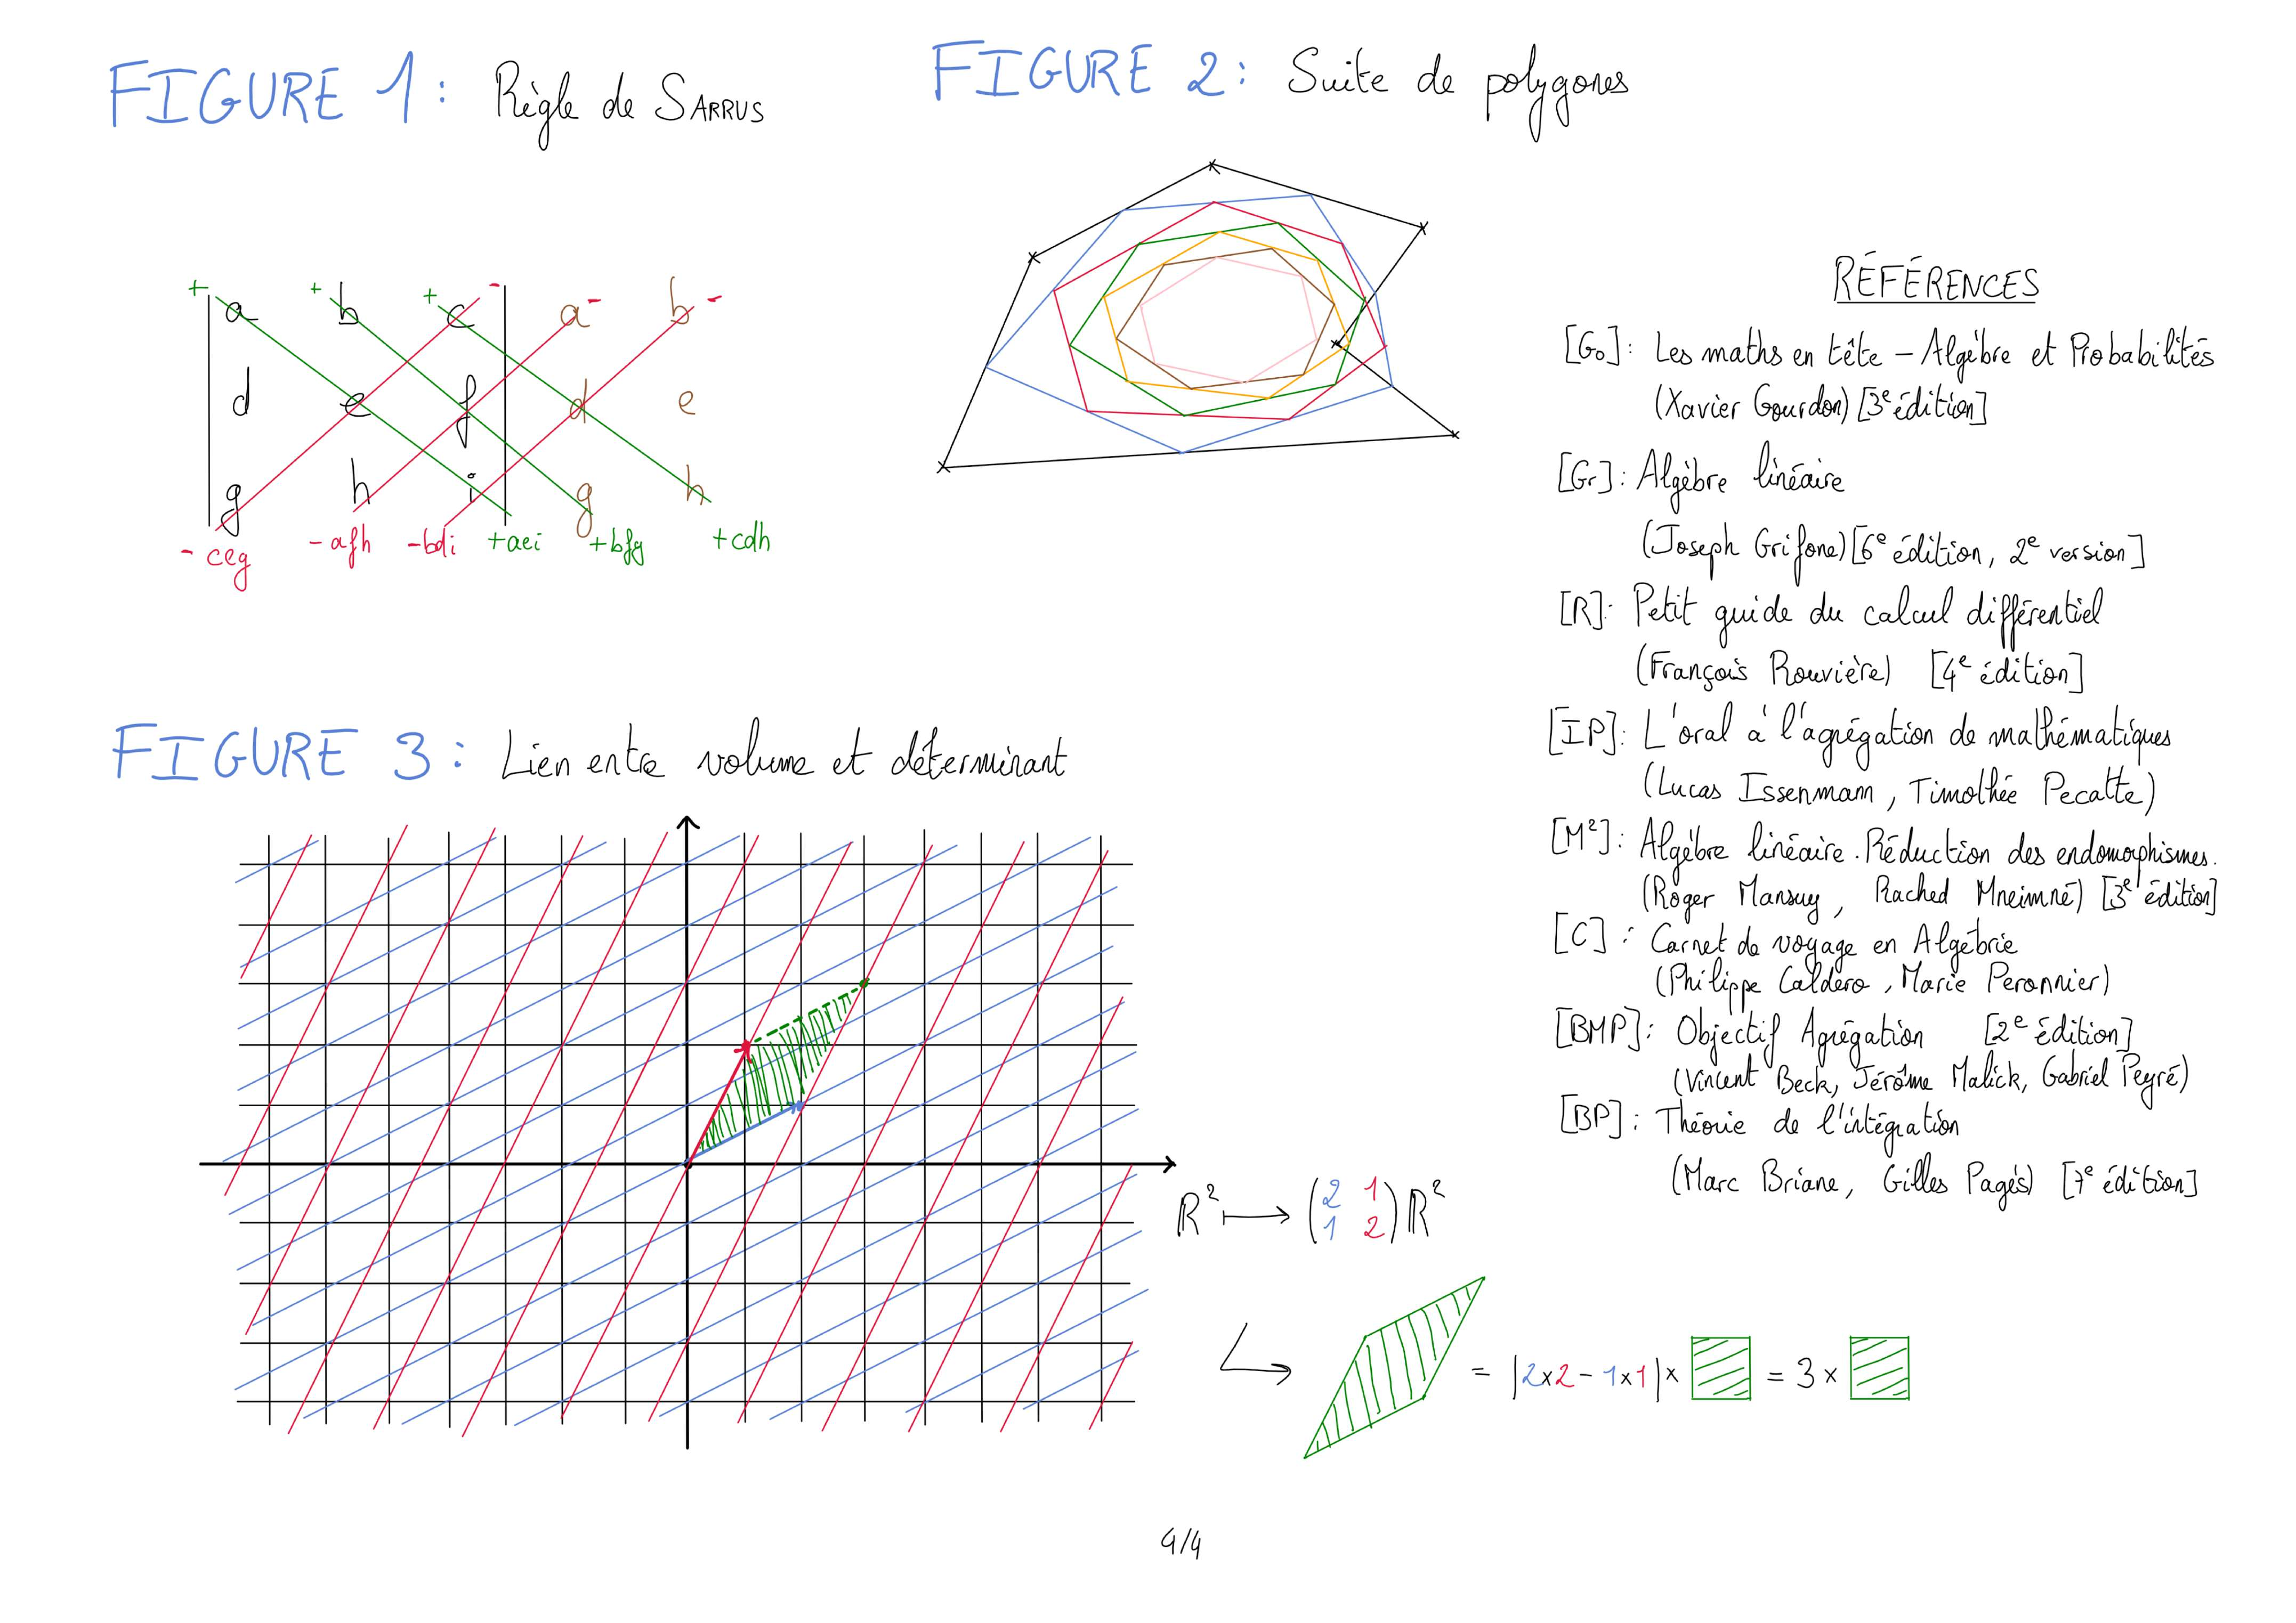
\includegraphics[trim={0 0 0 0},clip,width=1\linewidth]{img/149.pdf}
% 	\caption{s}
% \end{figure}
\end{document}

% \begin{tcolorbox}[
%     breakable, % Allows the theorem to split across pages
%     colback=developpement, % The background color
%     colframe=gray!0!black, % The frame color
%     boxrule=0pt, % The frame thickness
%     arc=1mm, % Sharp corners
% 	boxsep=0pt,
% 	left=0pt, right=0pt, top=0pt, bottom=0pt
% ]
% \end{tcolorbox}